\documentclass[twoside]{book}

% Packages required by doxygen
\usepackage{fixltx2e}
\usepackage{calc}
\usepackage{doxygen}
\usepackage[export]{adjustbox} % also loads graphicx
\usepackage{graphicx}
\usepackage[utf8]{inputenc}
\usepackage{makeidx}
\usepackage{multicol}
\usepackage{multirow}
\PassOptionsToPackage{warn}{textcomp}
\usepackage{textcomp}
\usepackage[nointegrals]{wasysym}
\usepackage[table]{xcolor}

% Font selection
\usepackage[T1]{fontenc}
\usepackage[scaled=.90]{helvet}
\usepackage{courier}
\usepackage{amssymb}
\usepackage{sectsty}
\renewcommand{\familydefault}{\sfdefault}
\allsectionsfont{%
  \fontseries{bc}\selectfont%
  \color{darkgray}%
}
\renewcommand{\DoxyLabelFont}{%
  \fontseries{bc}\selectfont%
  \color{darkgray}%
}
\newcommand{\+}{\discretionary{\mbox{\scriptsize$\hookleftarrow$}}{}{}}

% Page & text layout
\usepackage{geometry}
\geometry{%
  a4paper,%
  top=2.5cm,%
  bottom=2.5cm,%
  left=2.5cm,%
  right=2.5cm%
}
\tolerance=750
\hfuzz=15pt
\hbadness=750
\setlength{\emergencystretch}{15pt}
\setlength{\parindent}{0cm}
\setlength{\parskip}{3ex plus 2ex minus 2ex}
\makeatletter
\renewcommand{\paragraph}{%
  \@startsection{paragraph}{4}{0ex}{-1.0ex}{1.0ex}{%
    \normalfont\normalsize\bfseries\SS@parafont%
  }%
}
\renewcommand{\subparagraph}{%
  \@startsection{subparagraph}{5}{0ex}{-1.0ex}{1.0ex}{%
    \normalfont\normalsize\bfseries\SS@subparafont%
  }%
}
\makeatother

% Headers & footers
\usepackage{fancyhdr}
\pagestyle{fancyplain}
\fancyhead[LE]{\fancyplain{}{\bfseries\thepage}}
\fancyhead[CE]{\fancyplain{}{}}
\fancyhead[RE]{\fancyplain{}{\bfseries\leftmark}}
\fancyhead[LO]{\fancyplain{}{\bfseries\rightmark}}
\fancyhead[CO]{\fancyplain{}{}}
\fancyhead[RO]{\fancyplain{}{\bfseries\thepage}}
\fancyfoot[LE]{\fancyplain{}{}}
\fancyfoot[CE]{\fancyplain{}{}}
\fancyfoot[RE]{\fancyplain{}{\bfseries\scriptsize 構築\+: Doxygen }}
\fancyfoot[LO]{\fancyplain{}{\bfseries\scriptsize 構築\+: Doxygen }}
\fancyfoot[CO]{\fancyplain{}{}}
\fancyfoot[RO]{\fancyplain{}{}}
\renewcommand{\footrulewidth}{0.4pt}
\renewcommand{\chaptermark}[1]{%
  \markboth{#1}{}%
}
\renewcommand{\sectionmark}[1]{%
  \markright{\thesection\ #1}%
}

% Indices & bibliography
\usepackage{natbib}
\usepackage[titles]{tocloft}
\setcounter{tocdepth}{3}
\setcounter{secnumdepth}{5}
\makeindex

% Hyperlinks (required, but should be loaded last)
\usepackage{ifpdf}
\ifpdf
  \usepackage[pdftex,pagebackref=true]{hyperref}
\else
  \usepackage[ps2pdf,pagebackref=true]{hyperref}
\fi
\hypersetup{%
  colorlinks=true,%
  linkcolor=blue,%
  citecolor=blue,%
  unicode%
}

% Custom commands
\newcommand{\clearemptydoublepage}{%
  \newpage{\pagestyle{empty}\cleardoublepage}%
}

\usepackage{caption}
\captionsetup{labelsep=space,justification=centering,font={bf},singlelinecheck=off,skip=4pt,position=top}

%===== C O N T E N T S =====

\begin{document}

% Titlepage & ToC
\pagenumbering{alph}
\begin{titlepage}
\vspace*{7cm}
\begin{center}%
{\Large B\+E\+S\+I\+CE(Biped Exploration System In Complex Environment) \\[1ex]\large 1.\+0.\+0 }\\
\vspace*{1cm}
{\large 構築\+: Doxygen 1.8.13}\\
\end{center}
\end{titlepage}
\clearemptydoublepage
\pagenumbering{roman}
\tableofcontents
\clearemptydoublepage
\pagenumbering{arabic}

%--- Begin generated contents ---
\chapter{名前空間索引}
\section{名前空間一覧}
全名前空間の一覧です。\begin{DoxyCompactList}
\item\contentsline{section}{\hyperlink{namespacefractal}{fractal} }{\pageref{namespacefractal}}{}
\end{DoxyCompactList}

\chapter{階層索引}
\section{クラス階層}
クラス階層一覧です。大雑把に文字符号順で並べられています。\begin{DoxyCompactList}
\item \contentsline{section}{fractal\+:\+:baggage\+\_\+admin}{\pageref{classfractal_1_1baggage__admin}}{}
\begin{DoxyCompactList}
\item \contentsline{section}{fractal\+:\+:Module}{\pageref{classfractal_1_1Module}}{}
\begin{DoxyCompactList}
\item \contentsline{section}{fractal\+:\+:System}{\pageref{classfractal_1_1System}}{}
\end{DoxyCompactList}
\end{DoxyCompactList}
\item \contentsline{section}{fractal\+:\+:baggage\+\_\+component}{\pageref{classfractal_1_1baggage__component}}{}
\begin{DoxyCompactList}
\item \contentsline{section}{fractal\+:\+:baggage$<$ double $>$}{\pageref{classfractal_1_1baggage}}{}
\item \contentsline{section}{fractal\+:\+:baggage$<$ std\+:\+:string $>$}{\pageref{classfractal_1_1baggage}}{}
\item \contentsline{section}{fractal\+:\+:baggage$<$ T $>$}{\pageref{classfractal_1_1baggage}}{}
\end{DoxyCompactList}
\item \contentsline{section}{fractal\+:\+:Dummy}{\pageref{classfractal_1_1Dummy}}{}
\item \contentsline{section}{fractal\+:\+:baggage$<$ T $>$\+:\+:safe\+\_\+data}{\pageref{structfractal_1_1baggage_1_1safe__data}}{}
\end{DoxyCompactList}

\chapter{クラス索引}
\section{クラス一覧}
クラス・構造体・共用体・インターフェースの一覧です。\begin{DoxyCompactList}
\item\contentsline{section}{\hyperlink{classfractal_1_1baggage}{fractal\+::baggage$<$ T $>$} \\*Baggage Class }{\pageref{classfractal_1_1baggage}}{}
\item\contentsline{section}{\hyperlink{classfractal_1_1baggage__admin}{fractal\+::baggage\+\_\+admin} }{\pageref{classfractal_1_1baggage__admin}}{}
\item\contentsline{section}{\hyperlink{classfractal_1_1baggage__component}{fractal\+::baggage\+\_\+component} }{\pageref{classfractal_1_1baggage__component}}{}
\item\contentsline{section}{\hyperlink{classfractal_1_1Dummy}{fractal\+::\+Dummy} \\*Empty Class }{\pageref{classfractal_1_1Dummy}}{}
\item\contentsline{section}{\hyperlink{classfractal_1_1Module}{fractal\+::\+Module} \\*\hyperlink{classfractal_1_1Module}{Module} Class }{\pageref{classfractal_1_1Module}}{}
\item\contentsline{section}{\hyperlink{structfractal_1_1baggage_1_1safe__data}{fractal\+::baggage$<$ T $>$\+::safe\+\_\+data} \\*Safe data structure }{\pageref{structfractal_1_1baggage_1_1safe__data}}{}
\item\contentsline{section}{\hyperlink{classfractal_1_1System}{fractal\+::\+System} \\*\hyperlink{classfractal_1_1System}{System} Class }{\pageref{classfractal_1_1System}}{}
\end{DoxyCompactList}

\chapter{ファイル索引}
\section{ファイル一覧}
ファイル一覧です。\begin{DoxyCompactList}
\item\contentsline{section}{/home/takanobu/fractal/include/\hyperlink{fractal_8h}{fractal.\+h} \\*Parallel System Module }{\pageref{fractal_8h}}{}
\end{DoxyCompactList}

\chapter{名前空間詳解}
\section{fractal 名前空間}
\label{namespacefractal}\index{fractal@{fractal}}
\subsection*{クラス}
\begin{DoxyCompactItemize}
\item 
class \hyperlink{classfractal_1_1baggage}{baggage}
\begin{DoxyCompactList}\small\item\em Baggage Class \end{DoxyCompactList}\item 
class \hyperlink{classfractal_1_1baggage__admin}{baggage\+\_\+admin}
\item 
class \hyperlink{classfractal_1_1baggage__component}{baggage\+\_\+component}
\item 
class \hyperlink{classfractal_1_1Dummy}{Dummy}
\begin{DoxyCompactList}\small\item\em Empty Class \end{DoxyCompactList}\item 
class \hyperlink{classfractal_1_1Module}{Module}
\begin{DoxyCompactList}\small\item\em \hyperlink{classfractal_1_1Module}{Module} Class \end{DoxyCompactList}\item 
class \hyperlink{classfractal_1_1System}{System}
\begin{DoxyCompactList}\small\item\em \hyperlink{classfractal_1_1System}{System} Class \end{DoxyCompactList}\end{DoxyCompactItemize}
\subsection*{関数}
\begin{DoxyCompactItemize}
\item 
{\footnotesize template$<$class T $>$ }\\std\+::ostream \& \hyperlink{namespacefractal_abe8d2436bc90b6911384070a496cc49a}{operator$<$$<$} (std\+::ostream \&stream, \hyperlink{classfractal_1_1baggage}{baggage}$<$ T $>$ \&value)
\end{DoxyCompactItemize}
\subsection*{変数}
\begin{DoxyCompactItemize}
\item 
constexpr double \hyperlink{namespacefractal_aa98984c2091bb576a2063ed295e024f7}{gravity} = 9.\+80665
\end{DoxyCompactItemize}


\subsection{関数詳解}
\mbox{\label{namespacefractal_abe8d2436bc90b6911384070a496cc49a}} 
\index{fractal@{fractal}!operator$<$$<$@{operator$<$$<$}}
\index{operator$<$$<$@{operator$<$$<$}!fractal@{fractal}}
\subsubsection{\texorpdfstring{operator$<$$<$()}{operator<<()}}
{\footnotesize\ttfamily template$<$class T $>$ \\
std\+::ostream\& fractal\+::operator$<$$<$ (\begin{DoxyParamCaption}\item[{std\+::ostream \&}]{stream,  }\item[{\hyperlink{classfractal_1_1baggage}{baggage}$<$ T $>$ \&}]{value }\end{DoxyParamCaption})}



\subsection{変数詳解}
\mbox{\label{namespacefractal_aa98984c2091bb576a2063ed295e024f7}} 
\index{fractal@{fractal}!gravity@{gravity}}
\index{gravity@{gravity}!fractal@{fractal}}
\subsubsection{\texorpdfstring{gravity}{gravity}}
{\footnotesize\ttfamily constexpr double fractal\+::gravity = 9.\+80665}


\chapter{クラス詳解}
\section{fractal\+:\+:baggage$<$ T $>$ クラステンプレート}
\label{classfractal_1_1baggage}\index{fractal\+::baggage$<$ T $>$@{fractal\+::baggage$<$ T $>$}}


Baggage Class  




{\ttfamily \#include $<$fractal.\+h$>$}



fractal\+:\+:baggage$<$ T $>$ の継承関係図
\nopagebreak
\begin{figure}[H]
\begin{center}
\leavevmode
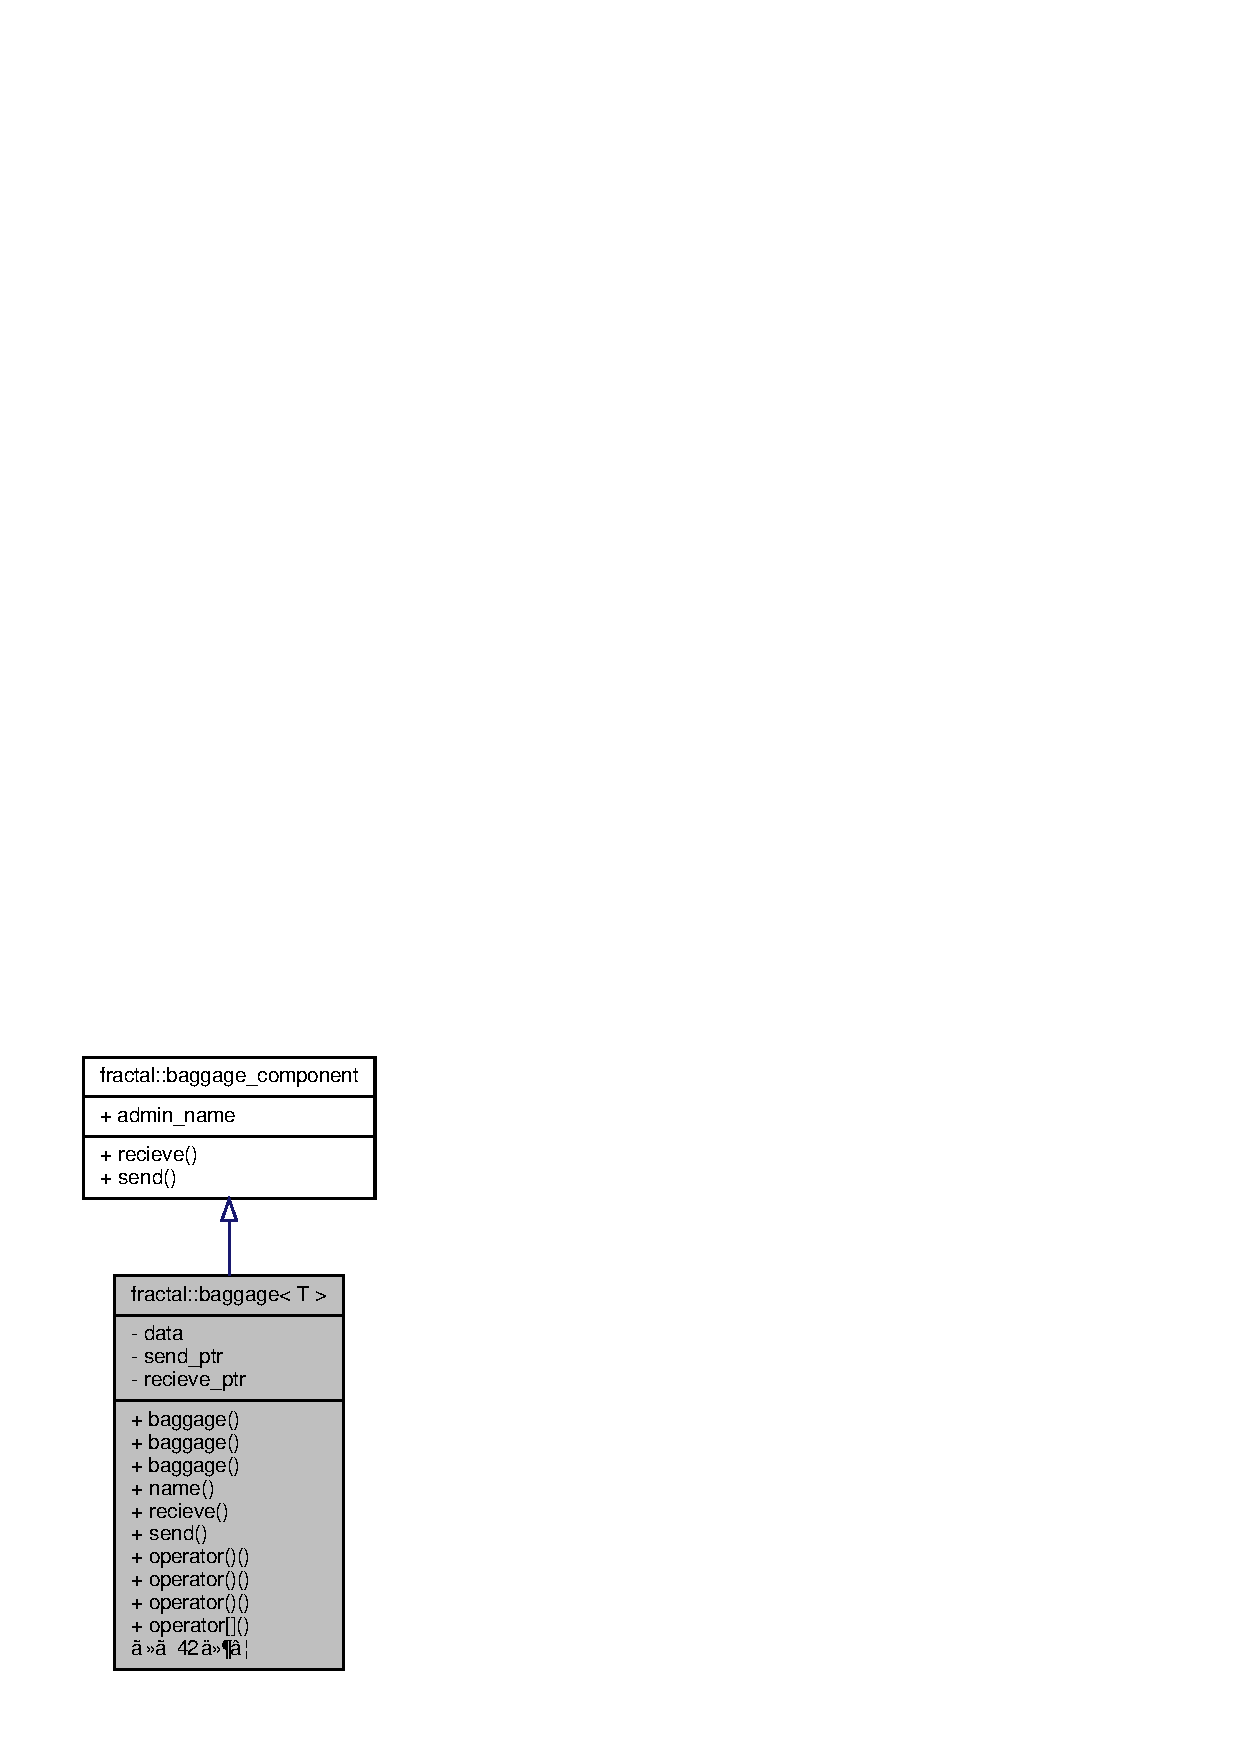
\includegraphics[width=184pt]{classfractal_1_1baggage__inherit__graph}
\end{center}
\end{figure}


fractal\+:\+:baggage$<$ T $>$ 連携図
\nopagebreak
\begin{figure}[H]
\begin{center}
\leavevmode
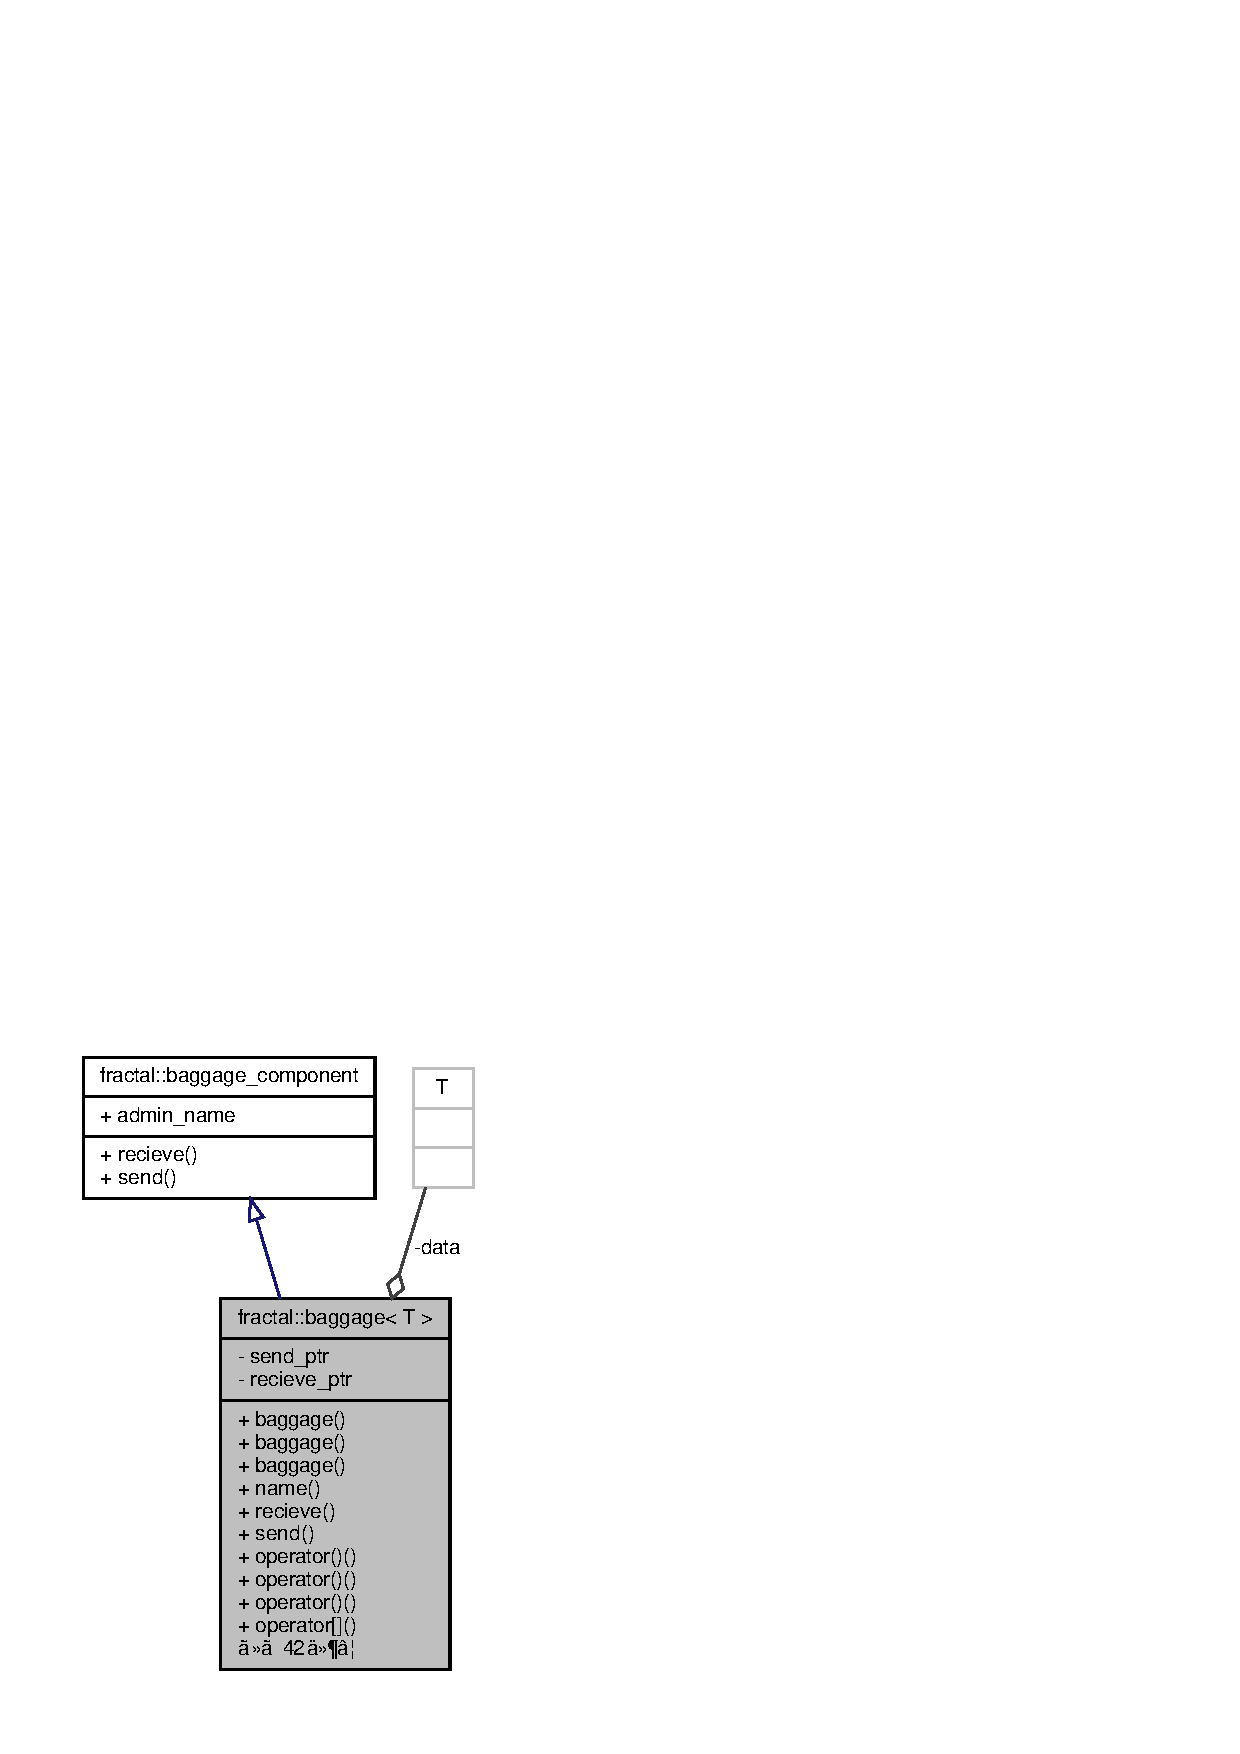
\includegraphics[width=232pt]{classfractal_1_1baggage__coll__graph}
\end{center}
\end{figure}
\subsection*{クラス}
\begin{DoxyCompactItemize}
\item 
struct \hyperlink{structfractal_1_1baggage_1_1safe__data}{safe\+\_\+data}
\begin{DoxyCompactList}\small\item\em safe data structure \end{DoxyCompactList}\end{DoxyCompactItemize}
\subsection*{公開メンバ関数}
\begin{DoxyCompactItemize}
\item 
\hyperlink{classfractal_1_1baggage_a4595c4e784aee7a446ef3e4ec4e25dbf}{baggage} ()
\item 
\hyperlink{classfractal_1_1baggage_a039105816c814c850137eb7ade424899}{baggage} (const auto \&v)
\item 
\hyperlink{classfractal_1_1baggage_ab3ab6b144d0fb9ee68d8f4810a4749f4}{baggage} (auto \&\&v)
\item 
std\+::string \hyperlink{classfractal_1_1baggage_ab9ce449071afe7e188a49d4a0be8d5f1}{name} (void)
\begin{DoxyCompactList}\small\item\em get class name of myself \end{DoxyCompactList}\item 
virtual void \hyperlink{classfractal_1_1baggage_aa7d07fc98f7c76789e6047345b2119ce}{recieve} (void)
\item 
virtual void \hyperlink{classfractal_1_1baggage_a12ef96c1b906369cfeeabdead61c257b}{send} (void)
\item 
T \& \hyperlink{classfractal_1_1baggage_a1ce803eda450dd559aa9b9818b28cf5e}{operator()} ()
\begin{DoxyCompactList}\small\item\em get data \end{DoxyCompactList}\item 
T \& \hyperlink{classfractal_1_1baggage_a3c94a35a361859fd455047a044213d01}{operator()} (const T \&d)
\begin{DoxyCompactList}\small\item\em set data \end{DoxyCompactList}\item 
T \& \hyperlink{classfractal_1_1baggage_a25086cfca4ea2ec94e9ee8965ce335c8}{operator()} (T \&\&d)
\begin{DoxyCompactList}\small\item\em set data \end{DoxyCompactList}\item 
auto \& \hyperlink{classfractal_1_1baggage_a00f2d4993290a8be28c911904637d178}{operator\mbox{[}$\,$\mbox{]}} (int n)
\item 
\hyperlink{classfractal_1_1baggage_a404f89564a219ffceb983cd3c77610e5}{operator T} ()
\begin{DoxyCompactList}\small\item\em cast \end{DoxyCompactList}\item 
T \hyperlink{classfractal_1_1baggage_aa196967bae7105ee4f7b2609557e3843}{operator=} (const auto \&d)
\begin{DoxyCompactList}\small\item\em set data \end{DoxyCompactList}\item 
T \hyperlink{classfractal_1_1baggage_a8904eb0c82e97fd1be2be7dbf9edf8a8}{operator=} (auto \&\&d)
\begin{DoxyCompactList}\small\item\em set data \end{DoxyCompactList}\item 
auto \hyperlink{classfractal_1_1baggage_a7e5735728eece548c425b12e45bb76ed}{operator+} (\hyperlink{classfractal_1_1baggage}{baggage} \&d)
\item 
auto \hyperlink{classfractal_1_1baggage_ae3e696df0f617540a076c098387c6df6}{operator-\/} (\hyperlink{classfractal_1_1baggage}{baggage} \&d)
\item 
auto \hyperlink{classfractal_1_1baggage_a65ff2c9d0b95c75913145564c916bb4e}{operator$\ast$} (\hyperlink{classfractal_1_1baggage}{baggage} \&d)
\item 
auto \hyperlink{classfractal_1_1baggage_a0011426532f94259bb3a737c26e4f9a8}{operator/} (\hyperlink{classfractal_1_1baggage}{baggage} \&d)
\item 
auto \hyperlink{classfractal_1_1baggage_a8a9085951c8eb400af15d2a9fd34e525}{operator+=} (\hyperlink{classfractal_1_1baggage}{baggage} \&d)
\item 
auto \hyperlink{classfractal_1_1baggage_a69180e126eca3a52976bf92dcf5fb998}{operator-\/=} (\hyperlink{classfractal_1_1baggage}{baggage} \&d)
\item 
auto \hyperlink{classfractal_1_1baggage_a4e874f81a01e3a13293163e4908eddf1}{operator$\ast$=} (\hyperlink{classfractal_1_1baggage}{baggage} \&d)
\item 
auto \hyperlink{classfractal_1_1baggage_a65c98b0f925e0c31d0d843a95aea5ffa}{operator/=} (\hyperlink{classfractal_1_1baggage}{baggage} \&d)
\item 
auto \hyperlink{classfractal_1_1baggage_a7a577be2bbc5619052bb8756c20ddb34}{operator+} (const auto \&d)
\item 
auto \hyperlink{classfractal_1_1baggage_a1c9f2aefd269f9338292f6075a575deb}{operator-\/} (const auto \&d)
\item 
auto \hyperlink{classfractal_1_1baggage_ac202db9fa4879077994458ed3e91967c}{operator$\ast$} (const auto \&d)
\item 
auto \hyperlink{classfractal_1_1baggage_a335eab1ed6f72d8c77229d31e78aa2de}{operator/} (const auto \&d)
\item 
auto \hyperlink{classfractal_1_1baggage_a6ad398719ada281520d99e1be3d040fa}{operator+} (auto \&\&d)
\item 
auto \hyperlink{classfractal_1_1baggage_ae897641772b637a6627626be213bc02d}{operator-\/} (auto \&\&d)
\item 
auto \hyperlink{classfractal_1_1baggage_ae5942f4512f10a45d544ab5752beab85}{operator$\ast$} (auto \&\&d)
\item 
auto \hyperlink{classfractal_1_1baggage_adab2ca242795c9a158c4f5948c8e29bb}{operator/} (auto \&\&d)
\item 
auto \hyperlink{classfractal_1_1baggage_ac97b2def4fa217147174cac53fc9cef8}{operator+=} (const auto \&d)
\item 
auto \hyperlink{classfractal_1_1baggage_aee89d99faea56059eb636574ebe20022}{operator-\/=} (const auto \&d)
\item 
auto \hyperlink{classfractal_1_1baggage_ac2a20d1eee27b24b907c33aacc1e0d0e}{operator$\ast$=} (const auto \&d)
\item 
auto \hyperlink{classfractal_1_1baggage_a94e6bca21db663f7fc5822e040ea122a}{operator/=} (const auto \&d)
\item 
auto \hyperlink{classfractal_1_1baggage_a5c290afd60258b17b78f85eee6dc022d}{operator+=} (auto \&\&d)
\item 
auto \hyperlink{classfractal_1_1baggage_a9d314a9b5b55481a6cb7b0aca2289276}{operator-\/=} (auto \&\&d)
\item 
auto \hyperlink{classfractal_1_1baggage_a13ad7848ea0bf14f49efc96149d95261}{operator$\ast$=} (auto \&\&d)
\item 
auto \hyperlink{classfractal_1_1baggage_aedd8c4c77dc0d2804fc5d6374524cd85}{operator/=} (auto \&\&d)
\item 
auto \hyperlink{classfractal_1_1baggage_a7ab638cfc6c7c77d20f84aa99e780da8}{operator++} ()
\item 
auto \hyperlink{classfractal_1_1baggage_a10b87d02b3423000f27c7f0970adffb8}{operator-\/-\/} ()
\item 
bool \hyperlink{classfractal_1_1baggage_ab193ca2ecc402a6f72cde64a12d9844d}{operator==} (const T \&d)
\item 
bool \hyperlink{classfractal_1_1baggage_a50e3b632e7803018ac854dcfd9d9d2f5}{operator!=} (const T \&d)
\item 
bool \hyperlink{classfractal_1_1baggage_a318fcecc8489897592370cf5c2edb588}{operator$<$} (const T \&d)
\item 
bool \hyperlink{classfractal_1_1baggage_a4493652a35653bf385084afbc26a7957}{operator$>$} (const T \&d)
\item 
bool \hyperlink{classfractal_1_1baggage_ab76eb0939f7a13f39ee721c1be8579bf}{operator$<$=} (const T \&d)
\item 
bool \hyperlink{classfractal_1_1baggage_a4552b3ca7b1aefaa892483d4c1694a3c}{operator$>$=} (const T \&d)
\item 
bool \hyperlink{classfractal_1_1baggage_af6cfa387876a27f6eab20938fc428d29}{operator==} (T \&\&d)
\item 
bool \hyperlink{classfractal_1_1baggage_ac4ef57664b87f4042451bbf431e03fa2}{operator!=} (T \&\&d)
\item 
bool \hyperlink{classfractal_1_1baggage_a249ba93cdd3c96fa0bdd13c6fe665ad7}{operator$<$} (T \&\&d)
\item 
bool \hyperlink{classfractal_1_1baggage_ae712ad4484a737818897ef6057253bcb}{operator$>$} (T \&\&d)
\item 
bool \hyperlink{classfractal_1_1baggage_af153cc94c9ec942b1165486192797326}{operator$<$=} (T \&\&d)
\item 
bool \hyperlink{classfractal_1_1baggage_ac1970dbf50991b785aa88707edce0e62}{operator$>$=} (T \&\&d)
\item 
\hyperlink{classfractal_1_1baggage}{baggage}$<$ T $>$ \& \hyperlink{classfractal_1_1baggage_aadd6a156f9116e6b9b4afa36ce998567}{operator$>$$>$} (\hyperlink{classfractal_1_1baggage}{baggage}$<$ T $>$ \&b)
\begin{DoxyCompactList}\small\item\em link data \end{DoxyCompactList}\end{DoxyCompactItemize}
\subsection*{非公開変数類}
\begin{DoxyCompactItemize}
\item 
T \hyperlink{classfractal_1_1baggage_a4ab1a1ce03c4f278087f62f7feac8cc3}{data}
\begin{DoxyCompactList}\small\item\em data \end{DoxyCompactList}\item 
std\+::shared\+\_\+ptr$<$ \hyperlink{structfractal_1_1baggage_1_1safe__data}{safe\+\_\+data} $>$ \hyperlink{classfractal_1_1baggage_aff8cc1cd923c97ecc18b7b574889ca63}{send\+\_\+ptr}
\begin{DoxyCompactList}\small\item\em send pointer \end{DoxyCompactList}\item 
std\+::weak\+\_\+ptr$<$ \hyperlink{structfractal_1_1baggage_1_1safe__data}{safe\+\_\+data} $>$ \hyperlink{classfractal_1_1baggage_ac6610690826b59751242686d488efe88}{recieve\+\_\+ptr}
\begin{DoxyCompactList}\small\item\em receive pointer \end{DoxyCompactList}\end{DoxyCompactItemize}
\subsection*{その他の継承メンバ}


\subsection{詳解}
\subsubsection*{template$<$class T$>$\newline
class fractal\+::baggage$<$ T $>$}

Baggage Class 


\begin{DoxyTemplParams}{Template Parameters}
{\em T} & type name\\
\hline
\end{DoxyTemplParams}
this class automatically performs exclusive processing 

\subsection{構築子と解体子}
\mbox{\label{classfractal_1_1baggage_a4595c4e784aee7a446ef3e4ec4e25dbf}} 
\index{fractal\+::baggage@{fractal\+::baggage}!baggage@{baggage}}
\index{baggage@{baggage}!fractal\+::baggage@{fractal\+::baggage}}
\subsubsection{\texorpdfstring{baggage()}{baggage()}\hspace{0.1cm}{\footnotesize\ttfamily [1/3]}}
{\footnotesize\ttfamily template$<$class T$>$ \\
\hyperlink{classfractal_1_1baggage}{fractal\+::baggage}$<$ T $>$\+::\hyperlink{classfractal_1_1baggage}{baggage} (\begin{DoxyParamCaption}{ }\end{DoxyParamCaption})\hspace{0.3cm}{\ttfamily [inline]}}

\mbox{\label{classfractal_1_1baggage_a039105816c814c850137eb7ade424899}} 
\index{fractal\+::baggage@{fractal\+::baggage}!baggage@{baggage}}
\index{baggage@{baggage}!fractal\+::baggage@{fractal\+::baggage}}
\subsubsection{\texorpdfstring{baggage()}{baggage()}\hspace{0.1cm}{\footnotesize\ttfamily [2/3]}}
{\footnotesize\ttfamily template$<$class T$>$ \\
\hyperlink{classfractal_1_1baggage}{fractal\+::baggage}$<$ T $>$\+::\hyperlink{classfractal_1_1baggage}{baggage} (\begin{DoxyParamCaption}\item[{const auto \&}]{v }\end{DoxyParamCaption})\hspace{0.3cm}{\ttfamily [inline]}}

\mbox{\label{classfractal_1_1baggage_ab3ab6b144d0fb9ee68d8f4810a4749f4}} 
\index{fractal\+::baggage@{fractal\+::baggage}!baggage@{baggage}}
\index{baggage@{baggage}!fractal\+::baggage@{fractal\+::baggage}}
\subsubsection{\texorpdfstring{baggage()}{baggage()}\hspace{0.1cm}{\footnotesize\ttfamily [3/3]}}
{\footnotesize\ttfamily template$<$class T$>$ \\
\hyperlink{classfractal_1_1baggage}{fractal\+::baggage}$<$ T $>$\+::\hyperlink{classfractal_1_1baggage}{baggage} (\begin{DoxyParamCaption}\item[{auto \&\&}]{v }\end{DoxyParamCaption})\hspace{0.3cm}{\ttfamily [inline]}}



\subsection{関数詳解}
\mbox{\label{classfractal_1_1baggage_ab9ce449071afe7e188a49d4a0be8d5f1}} 
\index{fractal\+::baggage@{fractal\+::baggage}!name@{name}}
\index{name@{name}!fractal\+::baggage@{fractal\+::baggage}}
\subsubsection{\texorpdfstring{name()}{name()}}
{\footnotesize\ttfamily template$<$class T$>$ \\
std\+::string \hyperlink{classfractal_1_1baggage}{fractal\+::baggage}$<$ T $>$\+::name (\begin{DoxyParamCaption}\item[{void}]{ }\end{DoxyParamCaption})\hspace{0.3cm}{\ttfamily [inline]}}



get class name of myself 

\begin{DoxyReturn}{戻り値}
class name 
\end{DoxyReturn}
\mbox{\label{classfractal_1_1baggage_a404f89564a219ffceb983cd3c77610e5}} 
\index{fractal\+::baggage@{fractal\+::baggage}!operator T@{operator T}}
\index{operator T@{operator T}!fractal\+::baggage@{fractal\+::baggage}}
\subsubsection{\texorpdfstring{operator T()}{operator T()}}
{\footnotesize\ttfamily template$<$class T$>$ \\
\hyperlink{classfractal_1_1baggage}{fractal\+::baggage}$<$ T $>$\+::operator T (\begin{DoxyParamCaption}{ }\end{DoxyParamCaption})\hspace{0.3cm}{\ttfamily [inline]}}



cast 

\mbox{\label{classfractal_1_1baggage_a50e3b632e7803018ac854dcfd9d9d2f5}} 
\index{fractal\+::baggage@{fractal\+::baggage}!operator"!=@{operator"!=}}
\index{operator"!=@{operator"!=}!fractal\+::baggage@{fractal\+::baggage}}
\subsubsection{\texorpdfstring{operator"!=()}{operator!=()}\hspace{0.1cm}{\footnotesize\ttfamily [1/2]}}
{\footnotesize\ttfamily template$<$class T$>$ \\
bool \hyperlink{classfractal_1_1baggage}{fractal\+::baggage}$<$ T $>$\+::operator!= (\begin{DoxyParamCaption}\item[{const T \&}]{d }\end{DoxyParamCaption})\hspace{0.3cm}{\ttfamily [inline]}}

\mbox{\label{classfractal_1_1baggage_ac4ef57664b87f4042451bbf431e03fa2}} 
\index{fractal\+::baggage@{fractal\+::baggage}!operator"!=@{operator"!=}}
\index{operator"!=@{operator"!=}!fractal\+::baggage@{fractal\+::baggage}}
\subsubsection{\texorpdfstring{operator"!=()}{operator!=()}\hspace{0.1cm}{\footnotesize\ttfamily [2/2]}}
{\footnotesize\ttfamily template$<$class T$>$ \\
bool \hyperlink{classfractal_1_1baggage}{fractal\+::baggage}$<$ T $>$\+::operator!= (\begin{DoxyParamCaption}\item[{T \&\&}]{d }\end{DoxyParamCaption})\hspace{0.3cm}{\ttfamily [inline]}}

\mbox{\label{classfractal_1_1baggage_a1ce803eda450dd559aa9b9818b28cf5e}} 
\index{fractal\+::baggage@{fractal\+::baggage}!operator()@{operator()}}
\index{operator()@{operator()}!fractal\+::baggage@{fractal\+::baggage}}
\subsubsection{\texorpdfstring{operator()()}{operator()()}\hspace{0.1cm}{\footnotesize\ttfamily [1/3]}}
{\footnotesize\ttfamily template$<$class T$>$ \\
T\& \hyperlink{classfractal_1_1baggage}{fractal\+::baggage}$<$ T $>$\+::operator() (\begin{DoxyParamCaption}{ }\end{DoxyParamCaption})\hspace{0.3cm}{\ttfamily [inline]}}



get data 

\mbox{\label{classfractal_1_1baggage_a3c94a35a361859fd455047a044213d01}} 
\index{fractal\+::baggage@{fractal\+::baggage}!operator()@{operator()}}
\index{operator()@{operator()}!fractal\+::baggage@{fractal\+::baggage}}
\subsubsection{\texorpdfstring{operator()()}{operator()()}\hspace{0.1cm}{\footnotesize\ttfamily [2/3]}}
{\footnotesize\ttfamily template$<$class T$>$ \\
T\& \hyperlink{classfractal_1_1baggage}{fractal\+::baggage}$<$ T $>$\+::operator() (\begin{DoxyParamCaption}\item[{const T \&}]{d }\end{DoxyParamCaption})\hspace{0.3cm}{\ttfamily [inline]}}



set data 

\mbox{\label{classfractal_1_1baggage_a25086cfca4ea2ec94e9ee8965ce335c8}} 
\index{fractal\+::baggage@{fractal\+::baggage}!operator()@{operator()}}
\index{operator()@{operator()}!fractal\+::baggage@{fractal\+::baggage}}
\subsubsection{\texorpdfstring{operator()()}{operator()()}\hspace{0.1cm}{\footnotesize\ttfamily [3/3]}}
{\footnotesize\ttfamily template$<$class T$>$ \\
T\& \hyperlink{classfractal_1_1baggage}{fractal\+::baggage}$<$ T $>$\+::operator() (\begin{DoxyParamCaption}\item[{T \&\&}]{d }\end{DoxyParamCaption})\hspace{0.3cm}{\ttfamily [inline]}}



set data 

\mbox{\label{classfractal_1_1baggage_a65ff2c9d0b95c75913145564c916bb4e}} 
\index{fractal\+::baggage@{fractal\+::baggage}!operator$\ast$@{operator$\ast$}}
\index{operator$\ast$@{operator$\ast$}!fractal\+::baggage@{fractal\+::baggage}}
\subsubsection{\texorpdfstring{operator$\ast$()}{operator*()}\hspace{0.1cm}{\footnotesize\ttfamily [1/3]}}
{\footnotesize\ttfamily template$<$class T$>$ \\
auto \hyperlink{classfractal_1_1baggage}{fractal\+::baggage}$<$ T $>$\+::operator$\ast$ (\begin{DoxyParamCaption}\item[{\hyperlink{classfractal_1_1baggage}{baggage}$<$ T $>$ \&}]{d }\end{DoxyParamCaption})\hspace{0.3cm}{\ttfamily [inline]}}

\mbox{\label{classfractal_1_1baggage_ac202db9fa4879077994458ed3e91967c}} 
\index{fractal\+::baggage@{fractal\+::baggage}!operator$\ast$@{operator$\ast$}}
\index{operator$\ast$@{operator$\ast$}!fractal\+::baggage@{fractal\+::baggage}}
\subsubsection{\texorpdfstring{operator$\ast$()}{operator*()}\hspace{0.1cm}{\footnotesize\ttfamily [2/3]}}
{\footnotesize\ttfamily template$<$class T$>$ \\
auto \hyperlink{classfractal_1_1baggage}{fractal\+::baggage}$<$ T $>$\+::operator$\ast$ (\begin{DoxyParamCaption}\item[{const auto \&}]{d }\end{DoxyParamCaption})\hspace{0.3cm}{\ttfamily [inline]}}

\mbox{\label{classfractal_1_1baggage_ae5942f4512f10a45d544ab5752beab85}} 
\index{fractal\+::baggage@{fractal\+::baggage}!operator$\ast$@{operator$\ast$}}
\index{operator$\ast$@{operator$\ast$}!fractal\+::baggage@{fractal\+::baggage}}
\subsubsection{\texorpdfstring{operator$\ast$()}{operator*()}\hspace{0.1cm}{\footnotesize\ttfamily [3/3]}}
{\footnotesize\ttfamily template$<$class T$>$ \\
auto \hyperlink{classfractal_1_1baggage}{fractal\+::baggage}$<$ T $>$\+::operator$\ast$ (\begin{DoxyParamCaption}\item[{auto \&\&}]{d }\end{DoxyParamCaption})\hspace{0.3cm}{\ttfamily [inline]}}

\mbox{\label{classfractal_1_1baggage_a4e874f81a01e3a13293163e4908eddf1}} 
\index{fractal\+::baggage@{fractal\+::baggage}!operator$\ast$=@{operator$\ast$=}}
\index{operator$\ast$=@{operator$\ast$=}!fractal\+::baggage@{fractal\+::baggage}}
\subsubsection{\texorpdfstring{operator$\ast$=()}{operator*=()}\hspace{0.1cm}{\footnotesize\ttfamily [1/3]}}
{\footnotesize\ttfamily template$<$class T$>$ \\
auto \hyperlink{classfractal_1_1baggage}{fractal\+::baggage}$<$ T $>$\+::operator$\ast$= (\begin{DoxyParamCaption}\item[{\hyperlink{classfractal_1_1baggage}{baggage}$<$ T $>$ \&}]{d }\end{DoxyParamCaption})\hspace{0.3cm}{\ttfamily [inline]}}

\mbox{\label{classfractal_1_1baggage_ac2a20d1eee27b24b907c33aacc1e0d0e}} 
\index{fractal\+::baggage@{fractal\+::baggage}!operator$\ast$=@{operator$\ast$=}}
\index{operator$\ast$=@{operator$\ast$=}!fractal\+::baggage@{fractal\+::baggage}}
\subsubsection{\texorpdfstring{operator$\ast$=()}{operator*=()}\hspace{0.1cm}{\footnotesize\ttfamily [2/3]}}
{\footnotesize\ttfamily template$<$class T$>$ \\
auto \hyperlink{classfractal_1_1baggage}{fractal\+::baggage}$<$ T $>$\+::operator$\ast$= (\begin{DoxyParamCaption}\item[{const auto \&}]{d }\end{DoxyParamCaption})\hspace{0.3cm}{\ttfamily [inline]}}

\mbox{\label{classfractal_1_1baggage_a13ad7848ea0bf14f49efc96149d95261}} 
\index{fractal\+::baggage@{fractal\+::baggage}!operator$\ast$=@{operator$\ast$=}}
\index{operator$\ast$=@{operator$\ast$=}!fractal\+::baggage@{fractal\+::baggage}}
\subsubsection{\texorpdfstring{operator$\ast$=()}{operator*=()}\hspace{0.1cm}{\footnotesize\ttfamily [3/3]}}
{\footnotesize\ttfamily template$<$class T$>$ \\
auto \hyperlink{classfractal_1_1baggage}{fractal\+::baggage}$<$ T $>$\+::operator$\ast$= (\begin{DoxyParamCaption}\item[{auto \&\&}]{d }\end{DoxyParamCaption})\hspace{0.3cm}{\ttfamily [inline]}}

\mbox{\label{classfractal_1_1baggage_a7e5735728eece548c425b12e45bb76ed}} 
\index{fractal\+::baggage@{fractal\+::baggage}!operator+@{operator+}}
\index{operator+@{operator+}!fractal\+::baggage@{fractal\+::baggage}}
\subsubsection{\texorpdfstring{operator+()}{operator+()}\hspace{0.1cm}{\footnotesize\ttfamily [1/3]}}
{\footnotesize\ttfamily template$<$class T$>$ \\
auto \hyperlink{classfractal_1_1baggage}{fractal\+::baggage}$<$ T $>$\+::operator+ (\begin{DoxyParamCaption}\item[{\hyperlink{classfractal_1_1baggage}{baggage}$<$ T $>$ \&}]{d }\end{DoxyParamCaption})\hspace{0.3cm}{\ttfamily [inline]}}

\mbox{\label{classfractal_1_1baggage_a7a577be2bbc5619052bb8756c20ddb34}} 
\index{fractal\+::baggage@{fractal\+::baggage}!operator+@{operator+}}
\index{operator+@{operator+}!fractal\+::baggage@{fractal\+::baggage}}
\subsubsection{\texorpdfstring{operator+()}{operator+()}\hspace{0.1cm}{\footnotesize\ttfamily [2/3]}}
{\footnotesize\ttfamily template$<$class T$>$ \\
auto \hyperlink{classfractal_1_1baggage}{fractal\+::baggage}$<$ T $>$\+::operator+ (\begin{DoxyParamCaption}\item[{const auto \&}]{d }\end{DoxyParamCaption})\hspace{0.3cm}{\ttfamily [inline]}}

\mbox{\label{classfractal_1_1baggage_a6ad398719ada281520d99e1be3d040fa}} 
\index{fractal\+::baggage@{fractal\+::baggage}!operator+@{operator+}}
\index{operator+@{operator+}!fractal\+::baggage@{fractal\+::baggage}}
\subsubsection{\texorpdfstring{operator+()}{operator+()}\hspace{0.1cm}{\footnotesize\ttfamily [3/3]}}
{\footnotesize\ttfamily template$<$class T$>$ \\
auto \hyperlink{classfractal_1_1baggage}{fractal\+::baggage}$<$ T $>$\+::operator+ (\begin{DoxyParamCaption}\item[{auto \&\&}]{d }\end{DoxyParamCaption})\hspace{0.3cm}{\ttfamily [inline]}}

\mbox{\label{classfractal_1_1baggage_a7ab638cfc6c7c77d20f84aa99e780da8}} 
\index{fractal\+::baggage@{fractal\+::baggage}!operator++@{operator++}}
\index{operator++@{operator++}!fractal\+::baggage@{fractal\+::baggage}}
\subsubsection{\texorpdfstring{operator++()}{operator++()}}
{\footnotesize\ttfamily template$<$class T$>$ \\
auto \hyperlink{classfractal_1_1baggage}{fractal\+::baggage}$<$ T $>$\+::operator++ (\begin{DoxyParamCaption}{ }\end{DoxyParamCaption})\hspace{0.3cm}{\ttfamily [inline]}}

\mbox{\label{classfractal_1_1baggage_a8a9085951c8eb400af15d2a9fd34e525}} 
\index{fractal\+::baggage@{fractal\+::baggage}!operator+=@{operator+=}}
\index{operator+=@{operator+=}!fractal\+::baggage@{fractal\+::baggage}}
\subsubsection{\texorpdfstring{operator+=()}{operator+=()}\hspace{0.1cm}{\footnotesize\ttfamily [1/3]}}
{\footnotesize\ttfamily template$<$class T$>$ \\
auto \hyperlink{classfractal_1_1baggage}{fractal\+::baggage}$<$ T $>$\+::operator+= (\begin{DoxyParamCaption}\item[{\hyperlink{classfractal_1_1baggage}{baggage}$<$ T $>$ \&}]{d }\end{DoxyParamCaption})\hspace{0.3cm}{\ttfamily [inline]}}

\mbox{\label{classfractal_1_1baggage_ac97b2def4fa217147174cac53fc9cef8}} 
\index{fractal\+::baggage@{fractal\+::baggage}!operator+=@{operator+=}}
\index{operator+=@{operator+=}!fractal\+::baggage@{fractal\+::baggage}}
\subsubsection{\texorpdfstring{operator+=()}{operator+=()}\hspace{0.1cm}{\footnotesize\ttfamily [2/3]}}
{\footnotesize\ttfamily template$<$class T$>$ \\
auto \hyperlink{classfractal_1_1baggage}{fractal\+::baggage}$<$ T $>$\+::operator+= (\begin{DoxyParamCaption}\item[{const auto \&}]{d }\end{DoxyParamCaption})\hspace{0.3cm}{\ttfamily [inline]}}

\mbox{\label{classfractal_1_1baggage_a5c290afd60258b17b78f85eee6dc022d}} 
\index{fractal\+::baggage@{fractal\+::baggage}!operator+=@{operator+=}}
\index{operator+=@{operator+=}!fractal\+::baggage@{fractal\+::baggage}}
\subsubsection{\texorpdfstring{operator+=()}{operator+=()}\hspace{0.1cm}{\footnotesize\ttfamily [3/3]}}
{\footnotesize\ttfamily template$<$class T$>$ \\
auto \hyperlink{classfractal_1_1baggage}{fractal\+::baggage}$<$ T $>$\+::operator+= (\begin{DoxyParamCaption}\item[{auto \&\&}]{d }\end{DoxyParamCaption})\hspace{0.3cm}{\ttfamily [inline]}}

\mbox{\label{classfractal_1_1baggage_ae3e696df0f617540a076c098387c6df6}} 
\index{fractal\+::baggage@{fractal\+::baggage}!operator-\/@{operator-\/}}
\index{operator-\/@{operator-\/}!fractal\+::baggage@{fractal\+::baggage}}
\subsubsection{\texorpdfstring{operator-\/()}{operator-()}\hspace{0.1cm}{\footnotesize\ttfamily [1/3]}}
{\footnotesize\ttfamily template$<$class T$>$ \\
auto \hyperlink{classfractal_1_1baggage}{fractal\+::baggage}$<$ T $>$\+::operator-\/ (\begin{DoxyParamCaption}\item[{\hyperlink{classfractal_1_1baggage}{baggage}$<$ T $>$ \&}]{d }\end{DoxyParamCaption})\hspace{0.3cm}{\ttfamily [inline]}}

\mbox{\label{classfractal_1_1baggage_a1c9f2aefd269f9338292f6075a575deb}} 
\index{fractal\+::baggage@{fractal\+::baggage}!operator-\/@{operator-\/}}
\index{operator-\/@{operator-\/}!fractal\+::baggage@{fractal\+::baggage}}
\subsubsection{\texorpdfstring{operator-\/()}{operator-()}\hspace{0.1cm}{\footnotesize\ttfamily [2/3]}}
{\footnotesize\ttfamily template$<$class T$>$ \\
auto \hyperlink{classfractal_1_1baggage}{fractal\+::baggage}$<$ T $>$\+::operator-\/ (\begin{DoxyParamCaption}\item[{const auto \&}]{d }\end{DoxyParamCaption})\hspace{0.3cm}{\ttfamily [inline]}}

\mbox{\label{classfractal_1_1baggage_ae897641772b637a6627626be213bc02d}} 
\index{fractal\+::baggage@{fractal\+::baggage}!operator-\/@{operator-\/}}
\index{operator-\/@{operator-\/}!fractal\+::baggage@{fractal\+::baggage}}
\subsubsection{\texorpdfstring{operator-\/()}{operator-()}\hspace{0.1cm}{\footnotesize\ttfamily [3/3]}}
{\footnotesize\ttfamily template$<$class T$>$ \\
auto \hyperlink{classfractal_1_1baggage}{fractal\+::baggage}$<$ T $>$\+::operator-\/ (\begin{DoxyParamCaption}\item[{auto \&\&}]{d }\end{DoxyParamCaption})\hspace{0.3cm}{\ttfamily [inline]}}

\mbox{\label{classfractal_1_1baggage_a10b87d02b3423000f27c7f0970adffb8}} 
\index{fractal\+::baggage@{fractal\+::baggage}!operator-\/-\/@{operator-\/-\/}}
\index{operator-\/-\/@{operator-\/-\/}!fractal\+::baggage@{fractal\+::baggage}}
\subsubsection{\texorpdfstring{operator-\/-\/()}{operator--()}}
{\footnotesize\ttfamily template$<$class T$>$ \\
auto \hyperlink{classfractal_1_1baggage}{fractal\+::baggage}$<$ T $>$\+::operator-\/-\/ (\begin{DoxyParamCaption}{ }\end{DoxyParamCaption})\hspace{0.3cm}{\ttfamily [inline]}}

\mbox{\label{classfractal_1_1baggage_a69180e126eca3a52976bf92dcf5fb998}} 
\index{fractal\+::baggage@{fractal\+::baggage}!operator-\/=@{operator-\/=}}
\index{operator-\/=@{operator-\/=}!fractal\+::baggage@{fractal\+::baggage}}
\subsubsection{\texorpdfstring{operator-\/=()}{operator-=()}\hspace{0.1cm}{\footnotesize\ttfamily [1/3]}}
{\footnotesize\ttfamily template$<$class T$>$ \\
auto \hyperlink{classfractal_1_1baggage}{fractal\+::baggage}$<$ T $>$\+::operator-\/= (\begin{DoxyParamCaption}\item[{\hyperlink{classfractal_1_1baggage}{baggage}$<$ T $>$ \&}]{d }\end{DoxyParamCaption})\hspace{0.3cm}{\ttfamily [inline]}}

\mbox{\label{classfractal_1_1baggage_aee89d99faea56059eb636574ebe20022}} 
\index{fractal\+::baggage@{fractal\+::baggage}!operator-\/=@{operator-\/=}}
\index{operator-\/=@{operator-\/=}!fractal\+::baggage@{fractal\+::baggage}}
\subsubsection{\texorpdfstring{operator-\/=()}{operator-=()}\hspace{0.1cm}{\footnotesize\ttfamily [2/3]}}
{\footnotesize\ttfamily template$<$class T$>$ \\
auto \hyperlink{classfractal_1_1baggage}{fractal\+::baggage}$<$ T $>$\+::operator-\/= (\begin{DoxyParamCaption}\item[{const auto \&}]{d }\end{DoxyParamCaption})\hspace{0.3cm}{\ttfamily [inline]}}

\mbox{\label{classfractal_1_1baggage_a9d314a9b5b55481a6cb7b0aca2289276}} 
\index{fractal\+::baggage@{fractal\+::baggage}!operator-\/=@{operator-\/=}}
\index{operator-\/=@{operator-\/=}!fractal\+::baggage@{fractal\+::baggage}}
\subsubsection{\texorpdfstring{operator-\/=()}{operator-=()}\hspace{0.1cm}{\footnotesize\ttfamily [3/3]}}
{\footnotesize\ttfamily template$<$class T$>$ \\
auto \hyperlink{classfractal_1_1baggage}{fractal\+::baggage}$<$ T $>$\+::operator-\/= (\begin{DoxyParamCaption}\item[{auto \&\&}]{d }\end{DoxyParamCaption})\hspace{0.3cm}{\ttfamily [inline]}}

\mbox{\label{classfractal_1_1baggage_a0011426532f94259bb3a737c26e4f9a8}} 
\index{fractal\+::baggage@{fractal\+::baggage}!operator/@{operator/}}
\index{operator/@{operator/}!fractal\+::baggage@{fractal\+::baggage}}
\subsubsection{\texorpdfstring{operator/()}{operator/()}\hspace{0.1cm}{\footnotesize\ttfamily [1/3]}}
{\footnotesize\ttfamily template$<$class T$>$ \\
auto \hyperlink{classfractal_1_1baggage}{fractal\+::baggage}$<$ T $>$\+::operator/ (\begin{DoxyParamCaption}\item[{\hyperlink{classfractal_1_1baggage}{baggage}$<$ T $>$ \&}]{d }\end{DoxyParamCaption})\hspace{0.3cm}{\ttfamily [inline]}}

\mbox{\label{classfractal_1_1baggage_a335eab1ed6f72d8c77229d31e78aa2de}} 
\index{fractal\+::baggage@{fractal\+::baggage}!operator/@{operator/}}
\index{operator/@{operator/}!fractal\+::baggage@{fractal\+::baggage}}
\subsubsection{\texorpdfstring{operator/()}{operator/()}\hspace{0.1cm}{\footnotesize\ttfamily [2/3]}}
{\footnotesize\ttfamily template$<$class T$>$ \\
auto \hyperlink{classfractal_1_1baggage}{fractal\+::baggage}$<$ T $>$\+::operator/ (\begin{DoxyParamCaption}\item[{const auto \&}]{d }\end{DoxyParamCaption})\hspace{0.3cm}{\ttfamily [inline]}}

\mbox{\label{classfractal_1_1baggage_adab2ca242795c9a158c4f5948c8e29bb}} 
\index{fractal\+::baggage@{fractal\+::baggage}!operator/@{operator/}}
\index{operator/@{operator/}!fractal\+::baggage@{fractal\+::baggage}}
\subsubsection{\texorpdfstring{operator/()}{operator/()}\hspace{0.1cm}{\footnotesize\ttfamily [3/3]}}
{\footnotesize\ttfamily template$<$class T$>$ \\
auto \hyperlink{classfractal_1_1baggage}{fractal\+::baggage}$<$ T $>$\+::operator/ (\begin{DoxyParamCaption}\item[{auto \&\&}]{d }\end{DoxyParamCaption})\hspace{0.3cm}{\ttfamily [inline]}}

\mbox{\label{classfractal_1_1baggage_a65c98b0f925e0c31d0d843a95aea5ffa}} 
\index{fractal\+::baggage@{fractal\+::baggage}!operator/=@{operator/=}}
\index{operator/=@{operator/=}!fractal\+::baggage@{fractal\+::baggage}}
\subsubsection{\texorpdfstring{operator/=()}{operator/=()}\hspace{0.1cm}{\footnotesize\ttfamily [1/3]}}
{\footnotesize\ttfamily template$<$class T$>$ \\
auto \hyperlink{classfractal_1_1baggage}{fractal\+::baggage}$<$ T $>$\+::operator/= (\begin{DoxyParamCaption}\item[{\hyperlink{classfractal_1_1baggage}{baggage}$<$ T $>$ \&}]{d }\end{DoxyParamCaption})\hspace{0.3cm}{\ttfamily [inline]}}

\mbox{\label{classfractal_1_1baggage_a94e6bca21db663f7fc5822e040ea122a}} 
\index{fractal\+::baggage@{fractal\+::baggage}!operator/=@{operator/=}}
\index{operator/=@{operator/=}!fractal\+::baggage@{fractal\+::baggage}}
\subsubsection{\texorpdfstring{operator/=()}{operator/=()}\hspace{0.1cm}{\footnotesize\ttfamily [2/3]}}
{\footnotesize\ttfamily template$<$class T$>$ \\
auto \hyperlink{classfractal_1_1baggage}{fractal\+::baggage}$<$ T $>$\+::operator/= (\begin{DoxyParamCaption}\item[{const auto \&}]{d }\end{DoxyParamCaption})\hspace{0.3cm}{\ttfamily [inline]}}

\mbox{\label{classfractal_1_1baggage_aedd8c4c77dc0d2804fc5d6374524cd85}} 
\index{fractal\+::baggage@{fractal\+::baggage}!operator/=@{operator/=}}
\index{operator/=@{operator/=}!fractal\+::baggage@{fractal\+::baggage}}
\subsubsection{\texorpdfstring{operator/=()}{operator/=()}\hspace{0.1cm}{\footnotesize\ttfamily [3/3]}}
{\footnotesize\ttfamily template$<$class T$>$ \\
auto \hyperlink{classfractal_1_1baggage}{fractal\+::baggage}$<$ T $>$\+::operator/= (\begin{DoxyParamCaption}\item[{auto \&\&}]{d }\end{DoxyParamCaption})\hspace{0.3cm}{\ttfamily [inline]}}

\mbox{\label{classfractal_1_1baggage_a318fcecc8489897592370cf5c2edb588}} 
\index{fractal\+::baggage@{fractal\+::baggage}!operator$<$@{operator$<$}}
\index{operator$<$@{operator$<$}!fractal\+::baggage@{fractal\+::baggage}}
\subsubsection{\texorpdfstring{operator$<$()}{operator<()}\hspace{0.1cm}{\footnotesize\ttfamily [1/2]}}
{\footnotesize\ttfamily template$<$class T$>$ \\
bool \hyperlink{classfractal_1_1baggage}{fractal\+::baggage}$<$ T $>$\+::operator$<$ (\begin{DoxyParamCaption}\item[{const T \&}]{d }\end{DoxyParamCaption})\hspace{0.3cm}{\ttfamily [inline]}}

\mbox{\label{classfractal_1_1baggage_a249ba93cdd3c96fa0bdd13c6fe665ad7}} 
\index{fractal\+::baggage@{fractal\+::baggage}!operator$<$@{operator$<$}}
\index{operator$<$@{operator$<$}!fractal\+::baggage@{fractal\+::baggage}}
\subsubsection{\texorpdfstring{operator$<$()}{operator<()}\hspace{0.1cm}{\footnotesize\ttfamily [2/2]}}
{\footnotesize\ttfamily template$<$class T$>$ \\
bool \hyperlink{classfractal_1_1baggage}{fractal\+::baggage}$<$ T $>$\+::operator$<$ (\begin{DoxyParamCaption}\item[{T \&\&}]{d }\end{DoxyParamCaption})\hspace{0.3cm}{\ttfamily [inline]}}

\mbox{\label{classfractal_1_1baggage_ab76eb0939f7a13f39ee721c1be8579bf}} 
\index{fractal\+::baggage@{fractal\+::baggage}!operator$<$=@{operator$<$=}}
\index{operator$<$=@{operator$<$=}!fractal\+::baggage@{fractal\+::baggage}}
\subsubsection{\texorpdfstring{operator$<$=()}{operator<=()}\hspace{0.1cm}{\footnotesize\ttfamily [1/2]}}
{\footnotesize\ttfamily template$<$class T$>$ \\
bool \hyperlink{classfractal_1_1baggage}{fractal\+::baggage}$<$ T $>$\+::operator$<$= (\begin{DoxyParamCaption}\item[{const T \&}]{d }\end{DoxyParamCaption})\hspace{0.3cm}{\ttfamily [inline]}}

\mbox{\label{classfractal_1_1baggage_af153cc94c9ec942b1165486192797326}} 
\index{fractal\+::baggage@{fractal\+::baggage}!operator$<$=@{operator$<$=}}
\index{operator$<$=@{operator$<$=}!fractal\+::baggage@{fractal\+::baggage}}
\subsubsection{\texorpdfstring{operator$<$=()}{operator<=()}\hspace{0.1cm}{\footnotesize\ttfamily [2/2]}}
{\footnotesize\ttfamily template$<$class T$>$ \\
bool \hyperlink{classfractal_1_1baggage}{fractal\+::baggage}$<$ T $>$\+::operator$<$= (\begin{DoxyParamCaption}\item[{T \&\&}]{d }\end{DoxyParamCaption})\hspace{0.3cm}{\ttfamily [inline]}}

\mbox{\label{classfractal_1_1baggage_aa196967bae7105ee4f7b2609557e3843}} 
\index{fractal\+::baggage@{fractal\+::baggage}!operator=@{operator=}}
\index{operator=@{operator=}!fractal\+::baggage@{fractal\+::baggage}}
\subsubsection{\texorpdfstring{operator=()}{operator=()}\hspace{0.1cm}{\footnotesize\ttfamily [1/2]}}
{\footnotesize\ttfamily template$<$class T$>$ \\
T \hyperlink{classfractal_1_1baggage}{fractal\+::baggage}$<$ T $>$\+::operator= (\begin{DoxyParamCaption}\item[{const auto \&}]{d }\end{DoxyParamCaption})\hspace{0.3cm}{\ttfamily [inline]}}



set data 

\mbox{\label{classfractal_1_1baggage_a8904eb0c82e97fd1be2be7dbf9edf8a8}} 
\index{fractal\+::baggage@{fractal\+::baggage}!operator=@{operator=}}
\index{operator=@{operator=}!fractal\+::baggage@{fractal\+::baggage}}
\subsubsection{\texorpdfstring{operator=()}{operator=()}\hspace{0.1cm}{\footnotesize\ttfamily [2/2]}}
{\footnotesize\ttfamily template$<$class T$>$ \\
T \hyperlink{classfractal_1_1baggage}{fractal\+::baggage}$<$ T $>$\+::operator= (\begin{DoxyParamCaption}\item[{auto \&\&}]{d }\end{DoxyParamCaption})\hspace{0.3cm}{\ttfamily [inline]}}



set data 

\mbox{\label{classfractal_1_1baggage_ab193ca2ecc402a6f72cde64a12d9844d}} 
\index{fractal\+::baggage@{fractal\+::baggage}!operator==@{operator==}}
\index{operator==@{operator==}!fractal\+::baggage@{fractal\+::baggage}}
\subsubsection{\texorpdfstring{operator==()}{operator==()}\hspace{0.1cm}{\footnotesize\ttfamily [1/2]}}
{\footnotesize\ttfamily template$<$class T$>$ \\
bool \hyperlink{classfractal_1_1baggage}{fractal\+::baggage}$<$ T $>$\+::operator== (\begin{DoxyParamCaption}\item[{const T \&}]{d }\end{DoxyParamCaption})\hspace{0.3cm}{\ttfamily [inline]}}

\mbox{\label{classfractal_1_1baggage_af6cfa387876a27f6eab20938fc428d29}} 
\index{fractal\+::baggage@{fractal\+::baggage}!operator==@{operator==}}
\index{operator==@{operator==}!fractal\+::baggage@{fractal\+::baggage}}
\subsubsection{\texorpdfstring{operator==()}{operator==()}\hspace{0.1cm}{\footnotesize\ttfamily [2/2]}}
{\footnotesize\ttfamily template$<$class T$>$ \\
bool \hyperlink{classfractal_1_1baggage}{fractal\+::baggage}$<$ T $>$\+::operator== (\begin{DoxyParamCaption}\item[{T \&\&}]{d }\end{DoxyParamCaption})\hspace{0.3cm}{\ttfamily [inline]}}

\mbox{\label{classfractal_1_1baggage_a4493652a35653bf385084afbc26a7957}} 
\index{fractal\+::baggage@{fractal\+::baggage}!operator$>$@{operator$>$}}
\index{operator$>$@{operator$>$}!fractal\+::baggage@{fractal\+::baggage}}
\subsubsection{\texorpdfstring{operator$>$()}{operator>()}\hspace{0.1cm}{\footnotesize\ttfamily [1/2]}}
{\footnotesize\ttfamily template$<$class T$>$ \\
bool \hyperlink{classfractal_1_1baggage}{fractal\+::baggage}$<$ T $>$\+::operator$>$ (\begin{DoxyParamCaption}\item[{const T \&}]{d }\end{DoxyParamCaption})\hspace{0.3cm}{\ttfamily [inline]}}

\mbox{\label{classfractal_1_1baggage_ae712ad4484a737818897ef6057253bcb}} 
\index{fractal\+::baggage@{fractal\+::baggage}!operator$>$@{operator$>$}}
\index{operator$>$@{operator$>$}!fractal\+::baggage@{fractal\+::baggage}}
\subsubsection{\texorpdfstring{operator$>$()}{operator>()}\hspace{0.1cm}{\footnotesize\ttfamily [2/2]}}
{\footnotesize\ttfamily template$<$class T$>$ \\
bool \hyperlink{classfractal_1_1baggage}{fractal\+::baggage}$<$ T $>$\+::operator$>$ (\begin{DoxyParamCaption}\item[{T \&\&}]{d }\end{DoxyParamCaption})\hspace{0.3cm}{\ttfamily [inline]}}

\mbox{\label{classfractal_1_1baggage_a4552b3ca7b1aefaa892483d4c1694a3c}} 
\index{fractal\+::baggage@{fractal\+::baggage}!operator$>$=@{operator$>$=}}
\index{operator$>$=@{operator$>$=}!fractal\+::baggage@{fractal\+::baggage}}
\subsubsection{\texorpdfstring{operator$>$=()}{operator>=()}\hspace{0.1cm}{\footnotesize\ttfamily [1/2]}}
{\footnotesize\ttfamily template$<$class T$>$ \\
bool \hyperlink{classfractal_1_1baggage}{fractal\+::baggage}$<$ T $>$\+::operator$>$= (\begin{DoxyParamCaption}\item[{const T \&}]{d }\end{DoxyParamCaption})\hspace{0.3cm}{\ttfamily [inline]}}

\mbox{\label{classfractal_1_1baggage_ac1970dbf50991b785aa88707edce0e62}} 
\index{fractal\+::baggage@{fractal\+::baggage}!operator$>$=@{operator$>$=}}
\index{operator$>$=@{operator$>$=}!fractal\+::baggage@{fractal\+::baggage}}
\subsubsection{\texorpdfstring{operator$>$=()}{operator>=()}\hspace{0.1cm}{\footnotesize\ttfamily [2/2]}}
{\footnotesize\ttfamily template$<$class T$>$ \\
bool \hyperlink{classfractal_1_1baggage}{fractal\+::baggage}$<$ T $>$\+::operator$>$= (\begin{DoxyParamCaption}\item[{T \&\&}]{d }\end{DoxyParamCaption})\hspace{0.3cm}{\ttfamily [inline]}}

\mbox{\label{classfractal_1_1baggage_aadd6a156f9116e6b9b4afa36ce998567}} 
\index{fractal\+::baggage@{fractal\+::baggage}!operator$>$$>$@{operator$>$$>$}}
\index{operator$>$$>$@{operator$>$$>$}!fractal\+::baggage@{fractal\+::baggage}}
\subsubsection{\texorpdfstring{operator$>$$>$()}{operator>>()}}
{\footnotesize\ttfamily template$<$class T$>$ \\
\hyperlink{classfractal_1_1baggage}{baggage}$<$T$>$\& \hyperlink{classfractal_1_1baggage}{fractal\+::baggage}$<$ T $>$\+::operator$>$$>$ (\begin{DoxyParamCaption}\item[{\hyperlink{classfractal_1_1baggage}{baggage}$<$ T $>$ \&}]{b }\end{DoxyParamCaption})\hspace{0.3cm}{\ttfamily [inline]}}



link data 

\mbox{\label{classfractal_1_1baggage_a00f2d4993290a8be28c911904637d178}} 
\index{fractal\+::baggage@{fractal\+::baggage}!operator\mbox{[}\mbox{]}@{operator[]}}
\index{operator\mbox{[}\mbox{]}@{operator[]}!fractal\+::baggage@{fractal\+::baggage}}
\subsubsection{\texorpdfstring{operator[]()}{operator[]()}}
{\footnotesize\ttfamily template$<$class T$>$ \\
auto\& \hyperlink{classfractal_1_1baggage}{fractal\+::baggage}$<$ T $>$\+::operator\mbox{[}$\,$\mbox{]} (\begin{DoxyParamCaption}\item[{int}]{n }\end{DoxyParamCaption})\hspace{0.3cm}{\ttfamily [inline]}}

\mbox{\label{classfractal_1_1baggage_aa7d07fc98f7c76789e6047345b2119ce}} 
\index{fractal\+::baggage@{fractal\+::baggage}!recieve@{recieve}}
\index{recieve@{recieve}!fractal\+::baggage@{fractal\+::baggage}}
\subsubsection{\texorpdfstring{recieve()}{recieve()}}
{\footnotesize\ttfamily template$<$class T$>$ \\
virtual void \hyperlink{classfractal_1_1baggage}{fractal\+::baggage}$<$ T $>$\+::recieve (\begin{DoxyParamCaption}\item[{void}]{ }\end{DoxyParamCaption})\hspace{0.3cm}{\ttfamily [inline]}, {\ttfamily [virtual]}}



\hyperlink{classfractal_1_1baggage__component_a37ef357c567ca8844d1b83c83e86df74}{fractal\+::baggage\+\_\+component}を再実装しています。

被呼び出し関係図\+:
\nopagebreak
\begin{figure}[H]
\begin{center}
\leavevmode
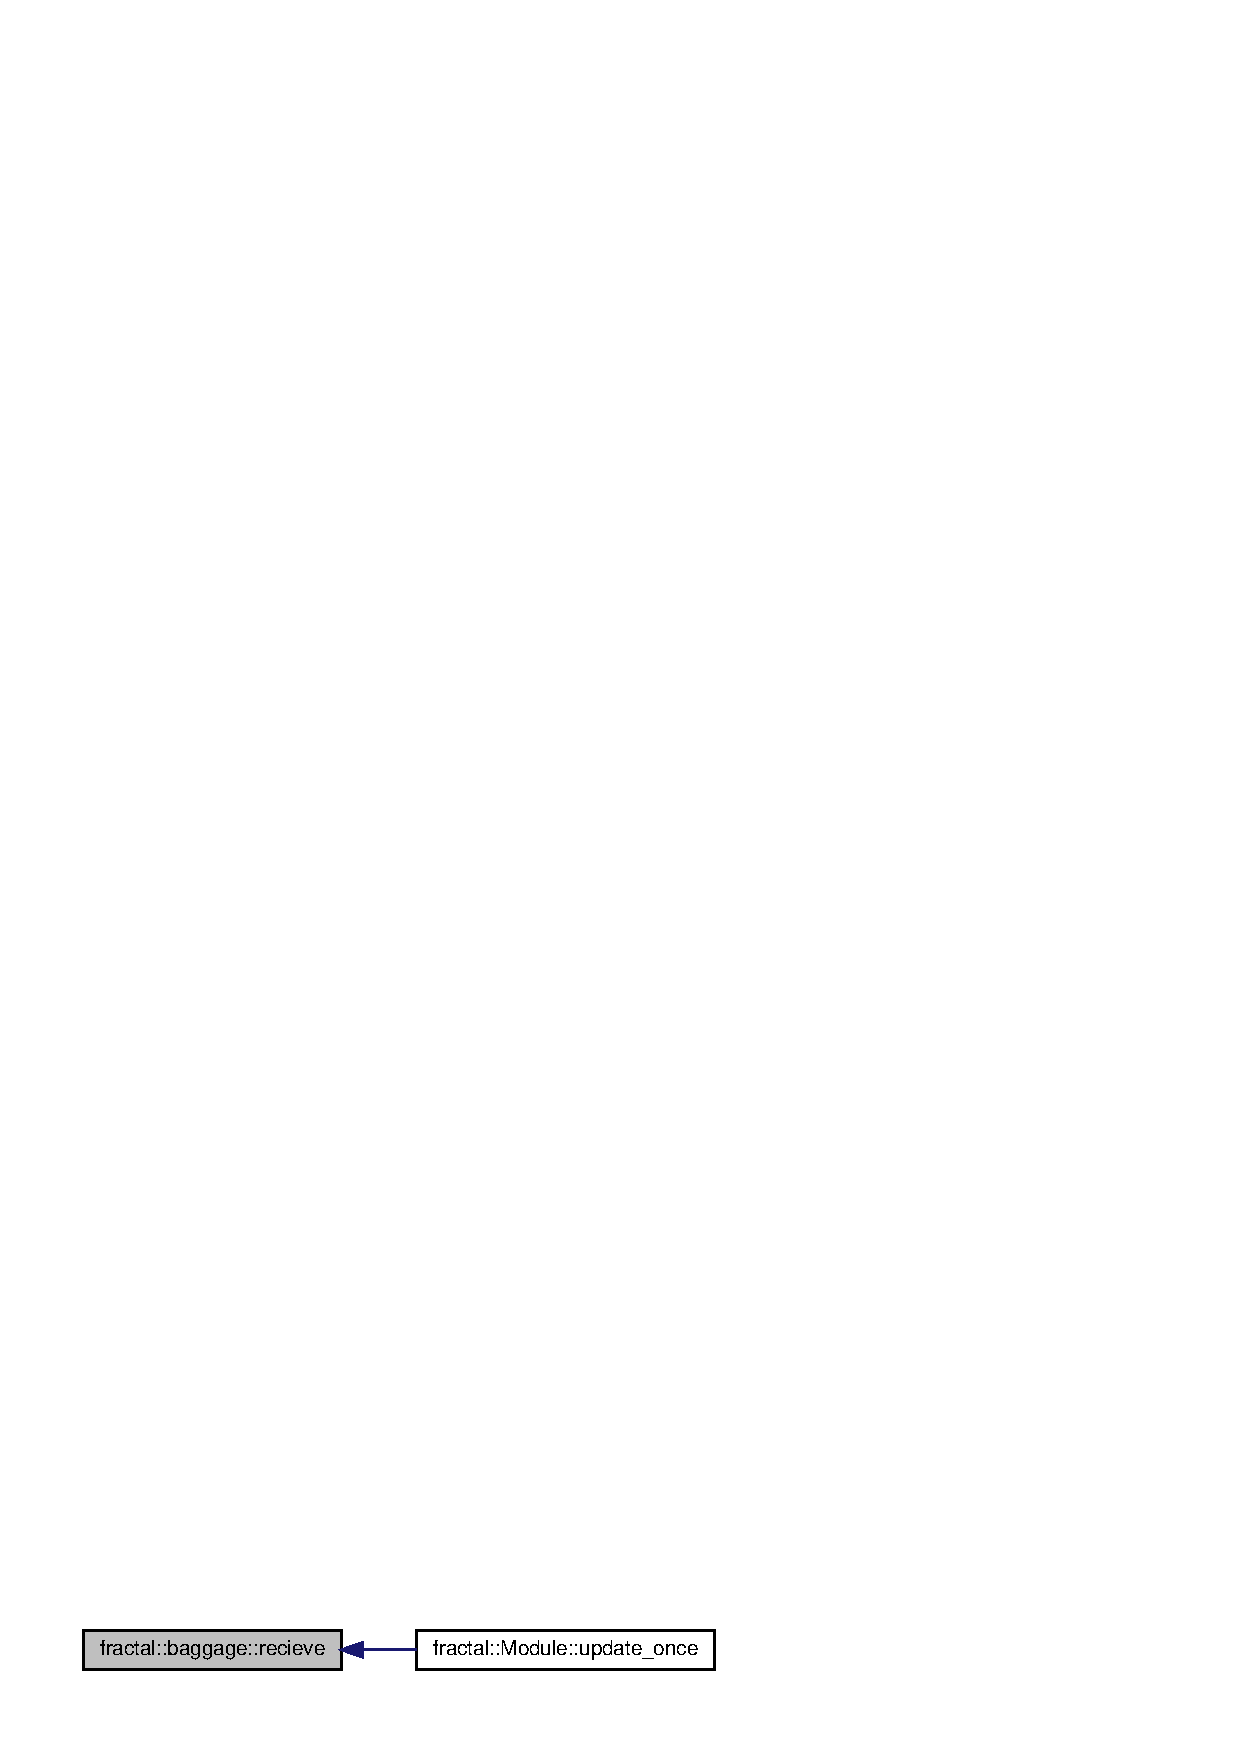
\includegraphics[width=347pt]{classfractal_1_1baggage_aa7d07fc98f7c76789e6047345b2119ce_icgraph}
\end{center}
\end{figure}
\mbox{\label{classfractal_1_1baggage_a12ef96c1b906369cfeeabdead61c257b}} 
\index{fractal\+::baggage@{fractal\+::baggage}!send@{send}}
\index{send@{send}!fractal\+::baggage@{fractal\+::baggage}}
\subsubsection{\texorpdfstring{send()}{send()}}
{\footnotesize\ttfamily template$<$class T$>$ \\
virtual void \hyperlink{classfractal_1_1baggage}{fractal\+::baggage}$<$ T $>$\+::send (\begin{DoxyParamCaption}\item[{void}]{ }\end{DoxyParamCaption})\hspace{0.3cm}{\ttfamily [inline]}, {\ttfamily [virtual]}}



\hyperlink{classfractal_1_1baggage__component_a8fdf9e534f892911e674de5a60eadf64}{fractal\+::baggage\+\_\+component}を再実装しています。

被呼び出し関係図\+:
\nopagebreak
\begin{figure}[H]
\begin{center}
\leavevmode
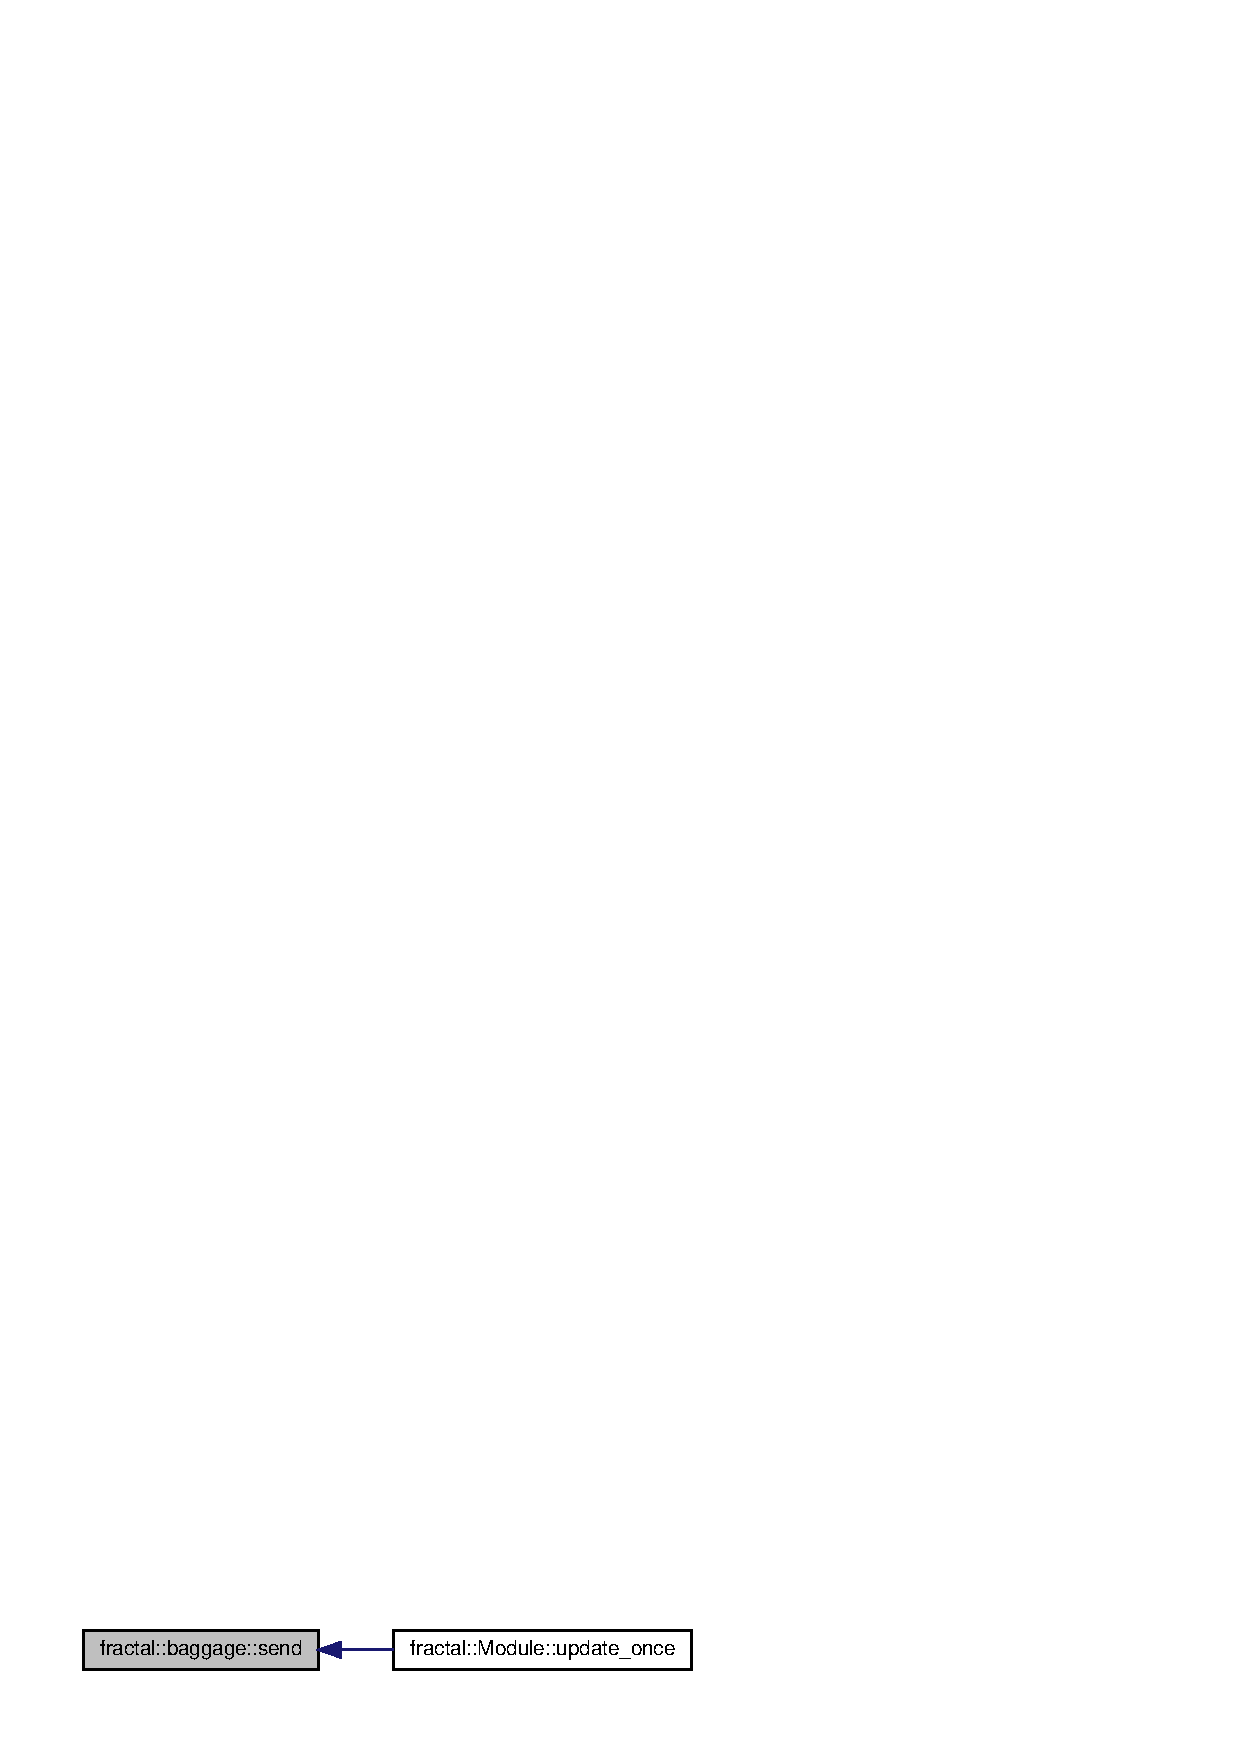
\includegraphics[width=336pt]{classfractal_1_1baggage_a12ef96c1b906369cfeeabdead61c257b_icgraph}
\end{center}
\end{figure}


\subsection{メンバ詳解}
\mbox{\label{classfractal_1_1baggage_a4ab1a1ce03c4f278087f62f7feac8cc3}} 
\index{fractal\+::baggage@{fractal\+::baggage}!data@{data}}
\index{data@{data}!fractal\+::baggage@{fractal\+::baggage}}
\subsubsection{\texorpdfstring{data}{data}}
{\footnotesize\ttfamily template$<$class T$>$ \\
T \hyperlink{classfractal_1_1baggage}{fractal\+::baggage}$<$ T $>$\+::data\hspace{0.3cm}{\ttfamily [private]}}



data 

\mbox{\label{classfractal_1_1baggage_ac6610690826b59751242686d488efe88}} 
\index{fractal\+::baggage@{fractal\+::baggage}!recieve\+\_\+ptr@{recieve\+\_\+ptr}}
\index{recieve\+\_\+ptr@{recieve\+\_\+ptr}!fractal\+::baggage@{fractal\+::baggage}}
\subsubsection{\texorpdfstring{recieve\+\_\+ptr}{recieve\_ptr}}
{\footnotesize\ttfamily template$<$class T$>$ \\
std\+::weak\+\_\+ptr$<$\hyperlink{structfractal_1_1baggage_1_1safe__data}{safe\+\_\+data}$>$ \hyperlink{classfractal_1_1baggage}{fractal\+::baggage}$<$ T $>$\+::recieve\+\_\+ptr\hspace{0.3cm}{\ttfamily [private]}}



receive pointer 

\mbox{\label{classfractal_1_1baggage_aff8cc1cd923c97ecc18b7b574889ca63}} 
\index{fractal\+::baggage@{fractal\+::baggage}!send\+\_\+ptr@{send\+\_\+ptr}}
\index{send\+\_\+ptr@{send\+\_\+ptr}!fractal\+::baggage@{fractal\+::baggage}}
\subsubsection{\texorpdfstring{send\+\_\+ptr}{send\_ptr}}
{\footnotesize\ttfamily template$<$class T$>$ \\
std\+::shared\+\_\+ptr$<$\hyperlink{structfractal_1_1baggage_1_1safe__data}{safe\+\_\+data}$>$ \hyperlink{classfractal_1_1baggage}{fractal\+::baggage}$<$ T $>$\+::send\+\_\+ptr\hspace{0.3cm}{\ttfamily [private]}}



send pointer 



このクラス詳解は次のファイルから抽出されました\+:\begin{DoxyCompactItemize}
\item 
/home/takanobu/fractal/include/\hyperlink{fractal_8h}{fractal.\+h}\end{DoxyCompactItemize}

\section{fractal\+:\+:baggage\+\_\+admin クラス}
\label{classfractal_1_1baggage__admin}\index{fractal\+::baggage\+\_\+admin@{fractal\+::baggage\+\_\+admin}}


{\ttfamily \#include $<$fractal.\+h$>$}



fractal\+:\+:baggage\+\_\+admin の継承関係図
\nopagebreak
\begin{figure}[H]
\begin{center}
\leavevmode
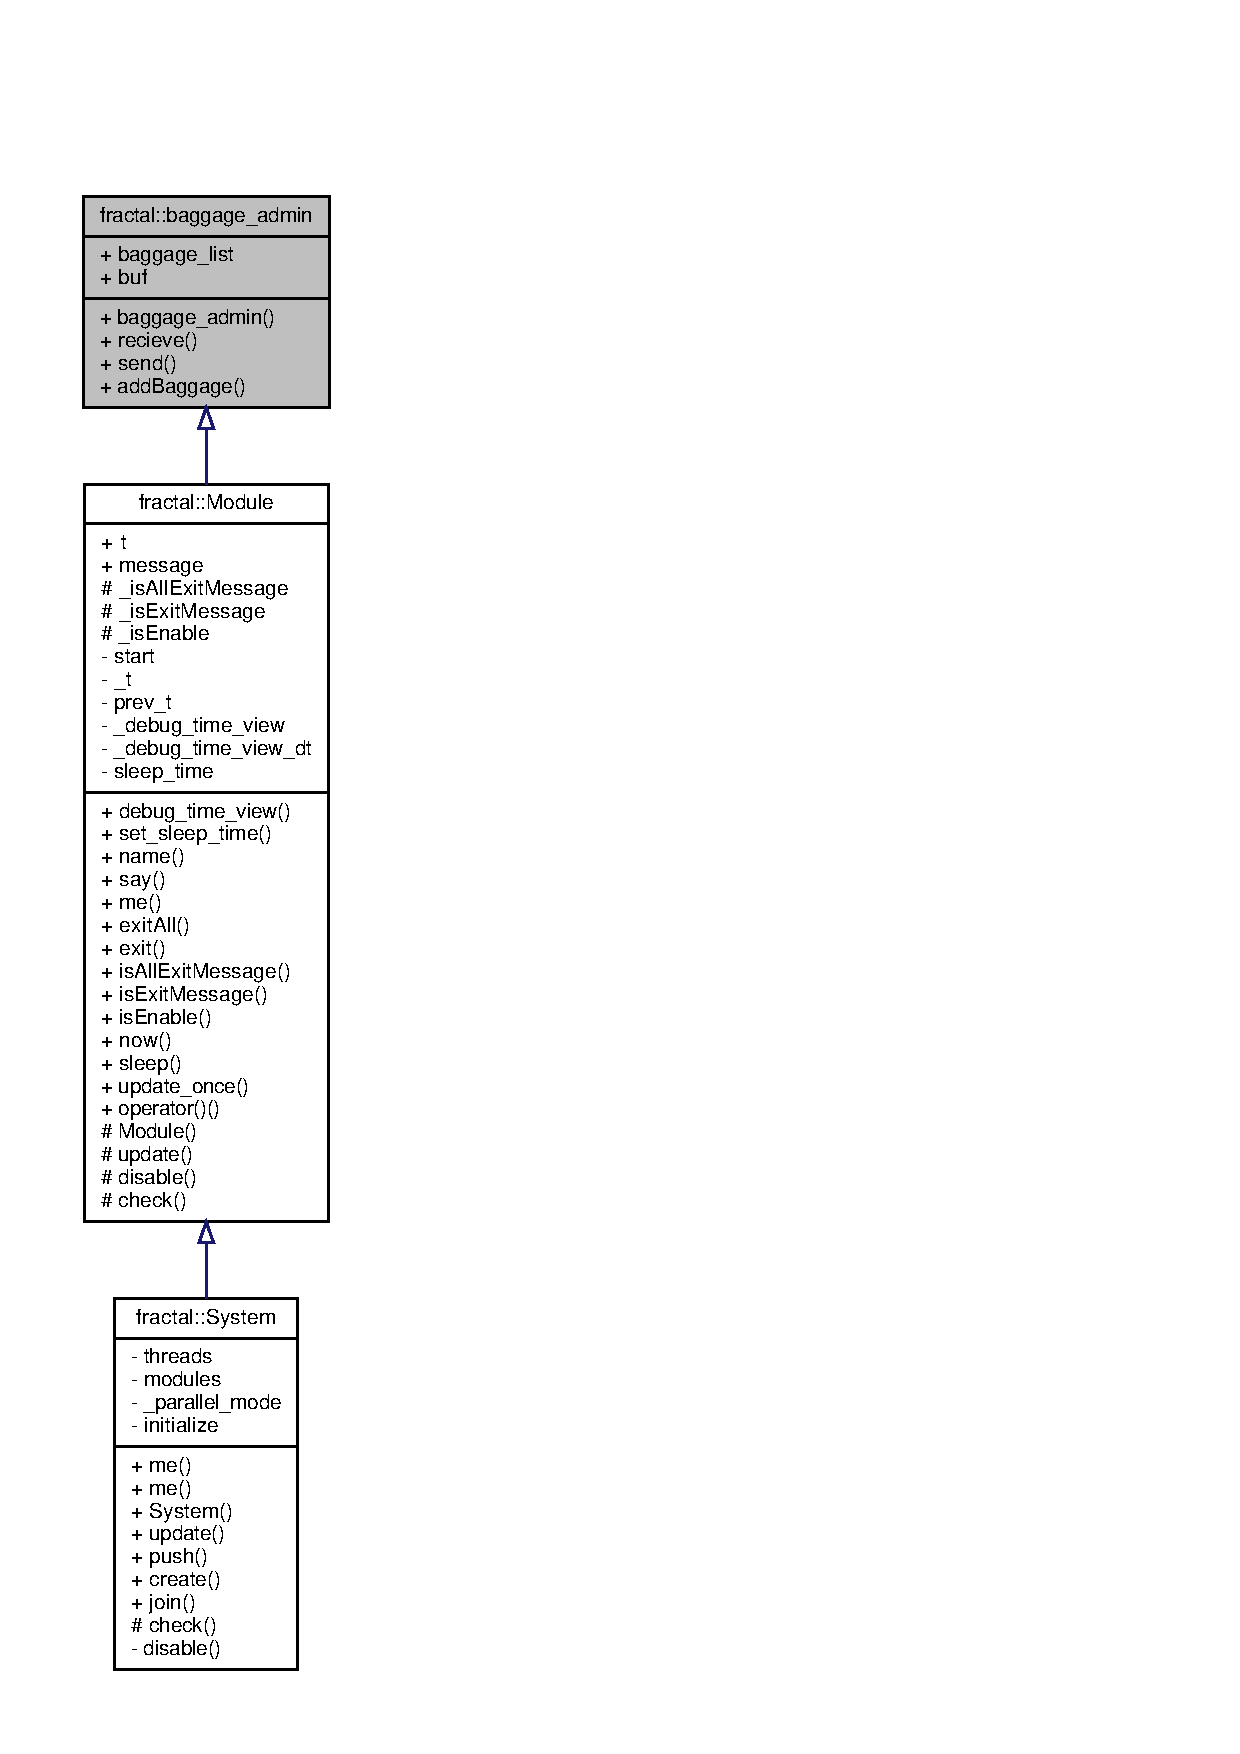
\includegraphics[height=550pt]{classfractal_1_1baggage__admin__inherit__graph}
\end{center}
\end{figure}


fractal\+:\+:baggage\+\_\+admin 連携図
\nopagebreak
\begin{figure}[H]
\begin{center}
\leavevmode
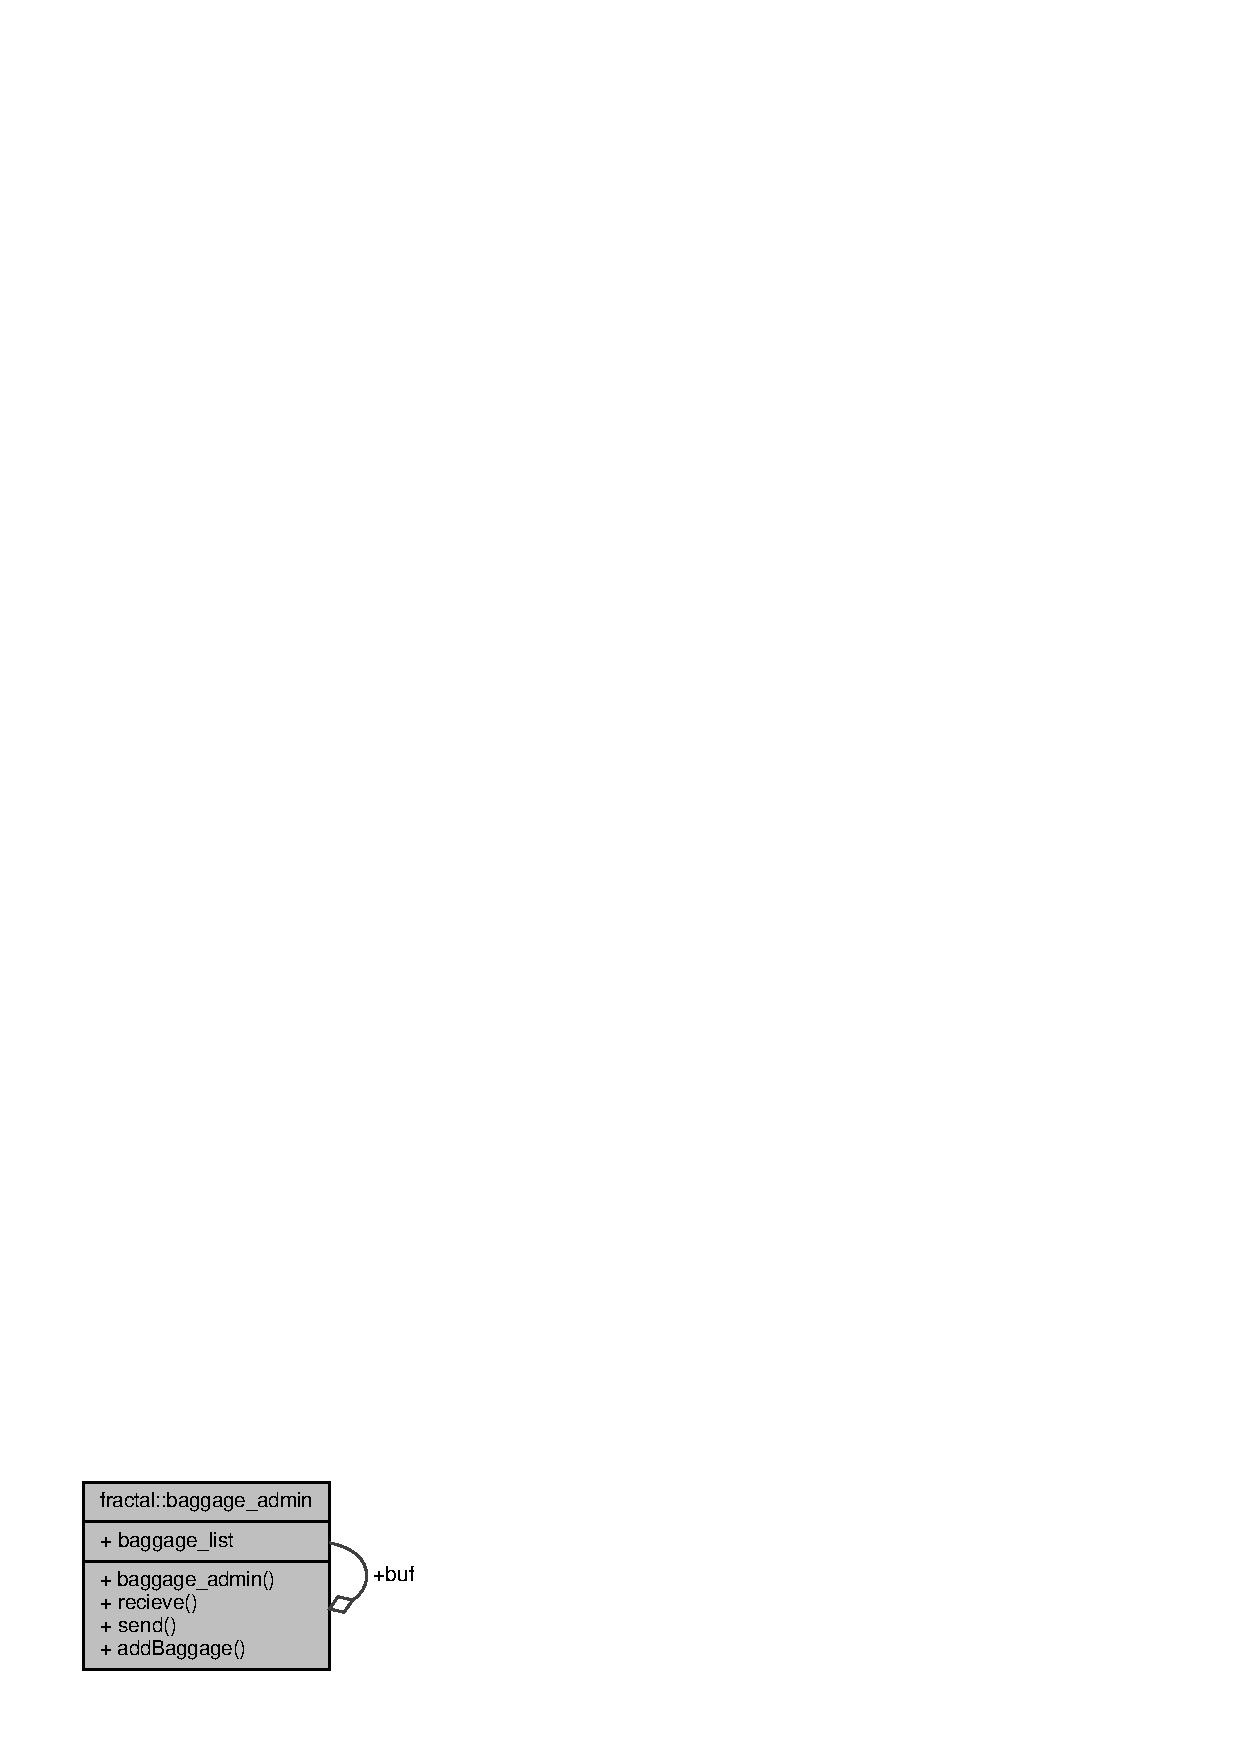
\includegraphics[width=203pt]{classfractal_1_1baggage__admin__coll__graph}
\end{center}
\end{figure}
\subsection*{公開メンバ関数}
\begin{DoxyCompactItemize}
\item 
\hyperlink{classfractal_1_1baggage__admin_a5f0d4b9b9fc7345b4686f5d9100137c0}{baggage\+\_\+admin} (void)
\item 
void \hyperlink{classfractal_1_1baggage__admin_a5ac84caf1682026eb58b319cae6289f3}{recieve} (void)
\item 
void \hyperlink{classfractal_1_1baggage__admin_a8fe4cbff60f094b3c659931c0cd3d251}{send} (void)
\item 
void \hyperlink{classfractal_1_1baggage__admin_a0d53a03fac20a4641edb09f4ad422ad2}{add\+Baggage} (\hyperlink{classfractal_1_1baggage__component}{baggage\+\_\+component} $\ast$ptr)
\end{DoxyCompactItemize}
\subsection*{公開変数類}
\begin{DoxyCompactItemize}
\item 
std\+::vector$<$ \hyperlink{classfractal_1_1baggage__component}{baggage\+\_\+component} $\ast$ $>$ \hyperlink{classfractal_1_1baggage__admin_afd92550fac7866335a3b55b78174887f}{baggage\+\_\+list}
\end{DoxyCompactItemize}
\subsection*{静的公開変数類}
\begin{DoxyCompactItemize}
\item 
static \hyperlink{classfractal_1_1baggage__admin}{baggage\+\_\+admin} $\ast$ \hyperlink{classfractal_1_1baggage__admin_a318bc60961b007f5430f859a6c9bba75}{buf}
\end{DoxyCompactItemize}


\subsection{構築子と解体子}
\mbox{\label{classfractal_1_1baggage__admin_a5f0d4b9b9fc7345b4686f5d9100137c0}} 
\index{fractal\+::baggage\+\_\+admin@{fractal\+::baggage\+\_\+admin}!baggage\+\_\+admin@{baggage\+\_\+admin}}
\index{baggage\+\_\+admin@{baggage\+\_\+admin}!fractal\+::baggage\+\_\+admin@{fractal\+::baggage\+\_\+admin}}
\subsubsection{\texorpdfstring{baggage\+\_\+admin()}{baggage\_admin()}}
{\footnotesize\ttfamily fractal\+::baggage\+\_\+admin\+::baggage\+\_\+admin (\begin{DoxyParamCaption}\item[{void}]{ }\end{DoxyParamCaption})\hspace{0.3cm}{\ttfamily [inline]}}



\subsection{関数詳解}
\mbox{\label{classfractal_1_1baggage__admin_a0d53a03fac20a4641edb09f4ad422ad2}} 
\index{fractal\+::baggage\+\_\+admin@{fractal\+::baggage\+\_\+admin}!add\+Baggage@{add\+Baggage}}
\index{add\+Baggage@{add\+Baggage}!fractal\+::baggage\+\_\+admin@{fractal\+::baggage\+\_\+admin}}
\subsubsection{\texorpdfstring{add\+Baggage()}{addBaggage()}}
{\footnotesize\ttfamily void fractal\+::baggage\+\_\+admin\+::add\+Baggage (\begin{DoxyParamCaption}\item[{\hyperlink{classfractal_1_1baggage__component}{baggage\+\_\+component} $\ast$}]{ptr }\end{DoxyParamCaption})\hspace{0.3cm}{\ttfamily [inline]}}

被呼び出し関係図\+:
\nopagebreak
\begin{figure}[H]
\begin{center}
\leavevmode
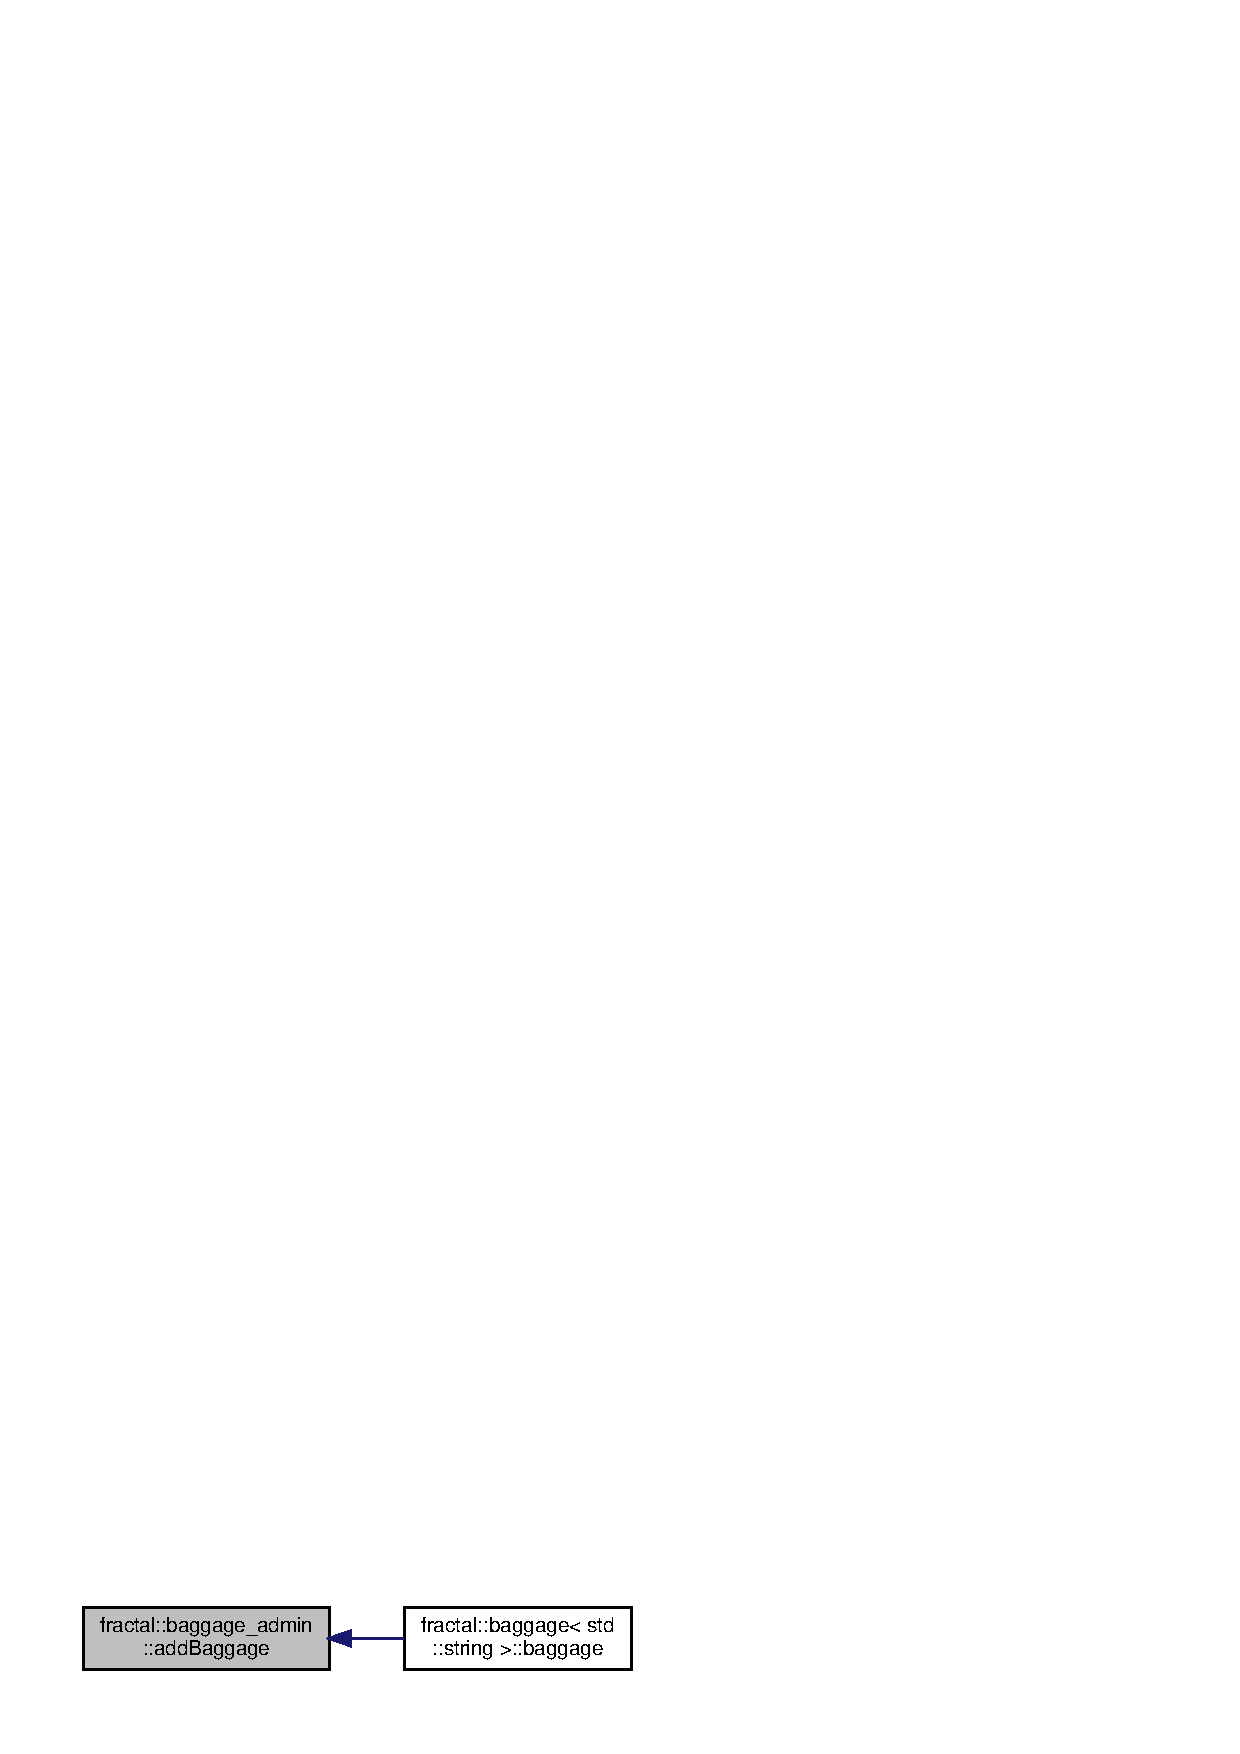
\includegraphics[width=307pt]{classfractal_1_1baggage__admin_a0d53a03fac20a4641edb09f4ad422ad2_icgraph}
\end{center}
\end{figure}
\mbox{\label{classfractal_1_1baggage__admin_a5ac84caf1682026eb58b319cae6289f3}} 
\index{fractal\+::baggage\+\_\+admin@{fractal\+::baggage\+\_\+admin}!recieve@{recieve}}
\index{recieve@{recieve}!fractal\+::baggage\+\_\+admin@{fractal\+::baggage\+\_\+admin}}
\subsubsection{\texorpdfstring{recieve()}{recieve()}}
{\footnotesize\ttfamily void fractal\+::baggage\+\_\+admin\+::recieve (\begin{DoxyParamCaption}\item[{void}]{ }\end{DoxyParamCaption})\hspace{0.3cm}{\ttfamily [inline]}}

\mbox{\label{classfractal_1_1baggage__admin_a8fe4cbff60f094b3c659931c0cd3d251}} 
\index{fractal\+::baggage\+\_\+admin@{fractal\+::baggage\+\_\+admin}!send@{send}}
\index{send@{send}!fractal\+::baggage\+\_\+admin@{fractal\+::baggage\+\_\+admin}}
\subsubsection{\texorpdfstring{send()}{send()}}
{\footnotesize\ttfamily void fractal\+::baggage\+\_\+admin\+::send (\begin{DoxyParamCaption}\item[{void}]{ }\end{DoxyParamCaption})\hspace{0.3cm}{\ttfamily [inline]}}

被呼び出し関係図\+:
\nopagebreak
\begin{figure}[H]
\begin{center}
\leavevmode
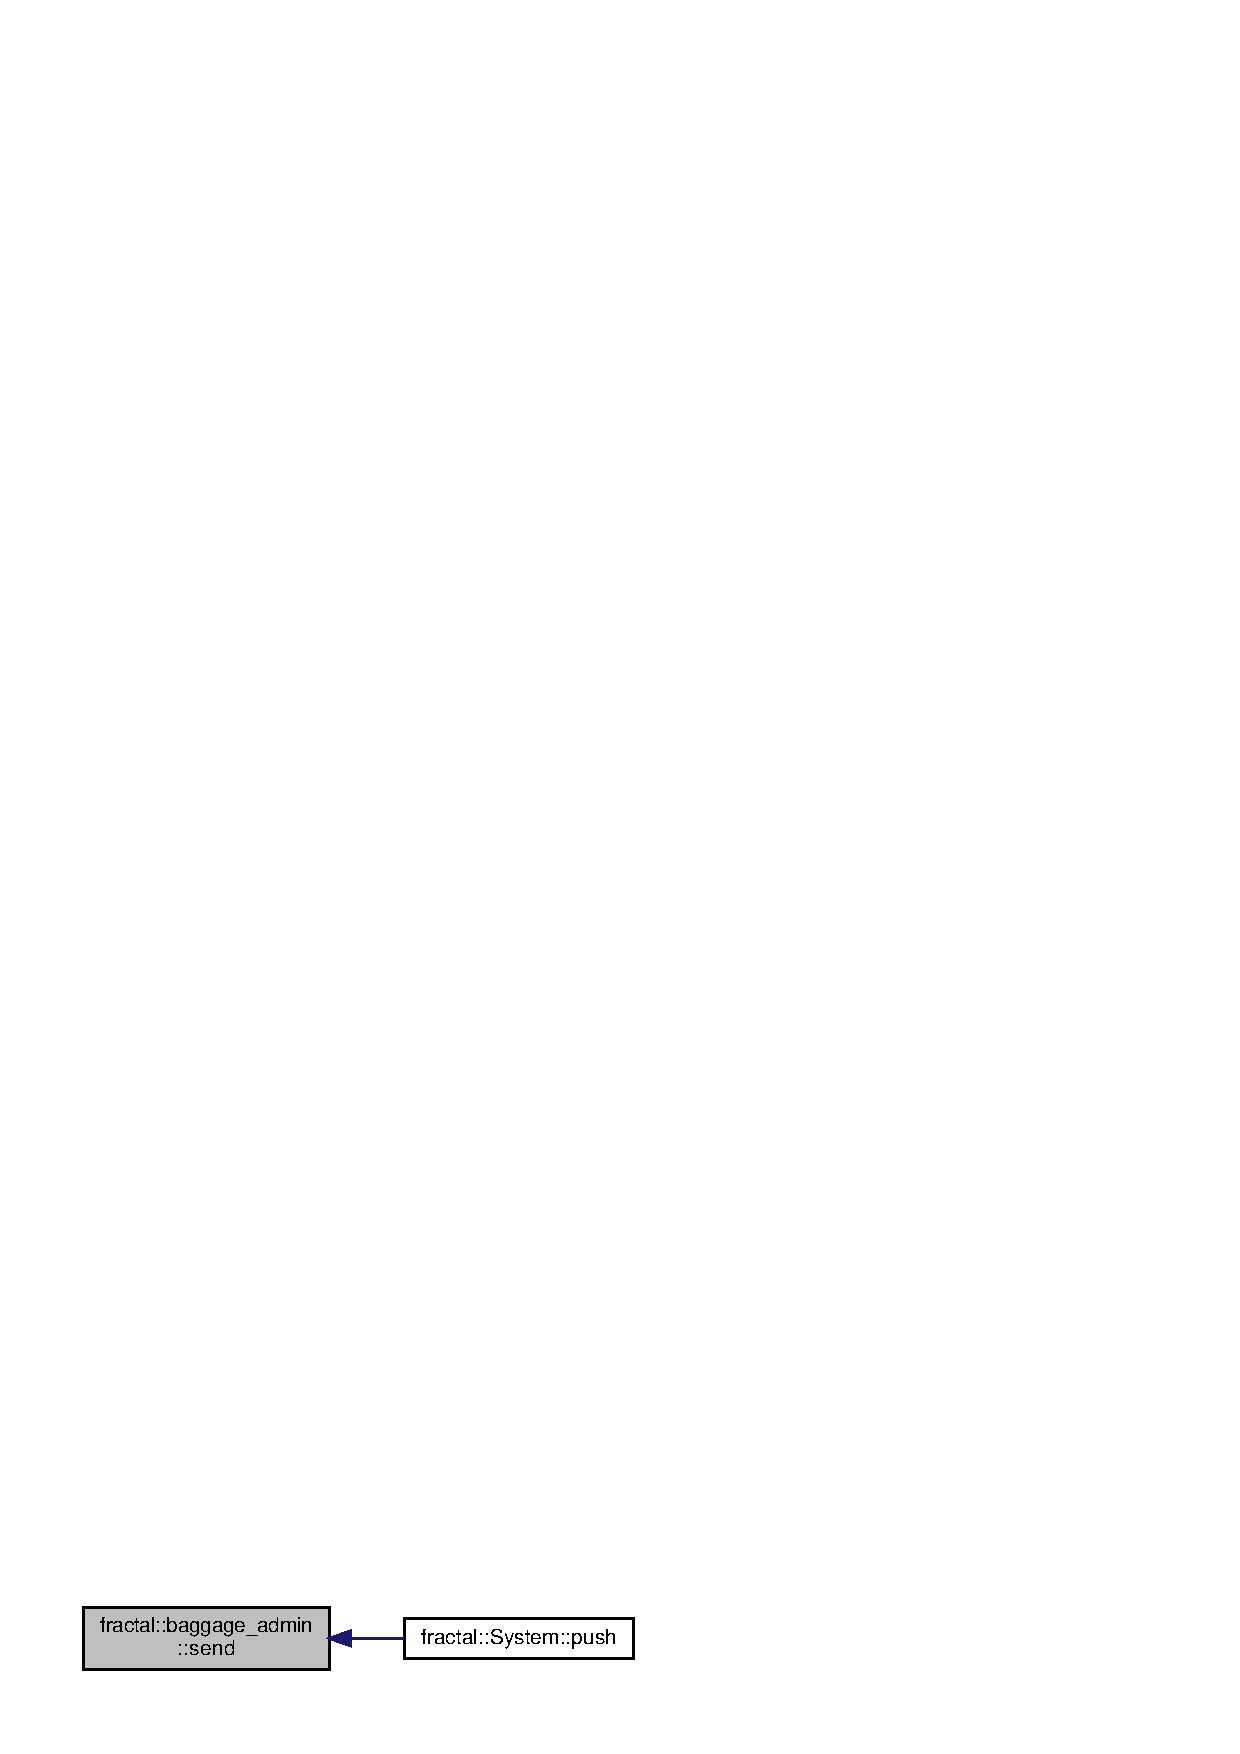
\includegraphics[width=308pt]{classfractal_1_1baggage__admin_a8fe4cbff60f094b3c659931c0cd3d251_icgraph}
\end{center}
\end{figure}


\subsection{メンバ詳解}
\mbox{\label{classfractal_1_1baggage__admin_afd92550fac7866335a3b55b78174887f}} 
\index{fractal\+::baggage\+\_\+admin@{fractal\+::baggage\+\_\+admin}!baggage\+\_\+list@{baggage\+\_\+list}}
\index{baggage\+\_\+list@{baggage\+\_\+list}!fractal\+::baggage\+\_\+admin@{fractal\+::baggage\+\_\+admin}}
\subsubsection{\texorpdfstring{baggage\+\_\+list}{baggage\_list}}
{\footnotesize\ttfamily std\+::vector$<$\hyperlink{classfractal_1_1baggage__component}{baggage\+\_\+component} $\ast$$>$ fractal\+::baggage\+\_\+admin\+::baggage\+\_\+list}

\mbox{\label{classfractal_1_1baggage__admin_a318bc60961b007f5430f859a6c9bba75}} 
\index{fractal\+::baggage\+\_\+admin@{fractal\+::baggage\+\_\+admin}!buf@{buf}}
\index{buf@{buf}!fractal\+::baggage\+\_\+admin@{fractal\+::baggage\+\_\+admin}}
\subsubsection{\texorpdfstring{buf}{buf}}
{\footnotesize\ttfamily \hyperlink{classfractal_1_1baggage__admin}{baggage\+\_\+admin} $\ast$ fractal\+::baggage\+\_\+admin\+::buf\hspace{0.3cm}{\ttfamily [static]}}



このクラス詳解は次のファイルから抽出されました\+:\begin{DoxyCompactItemize}
\item 
/home/takanobu/fractal/include/\hyperlink{fractal_8h}{fractal.\+h}\end{DoxyCompactItemize}

\section{fractal\+:\+:baggage\+\_\+component クラス}
\label{classfractal_1_1baggage__component}\index{fractal\+::baggage\+\_\+component@{fractal\+::baggage\+\_\+component}}


{\ttfamily \#include $<$fractal.\+h$>$}



fractal\+:\+:baggage\+\_\+component の継承関係図
\nopagebreak
\begin{figure}[H]
\begin{center}
\leavevmode
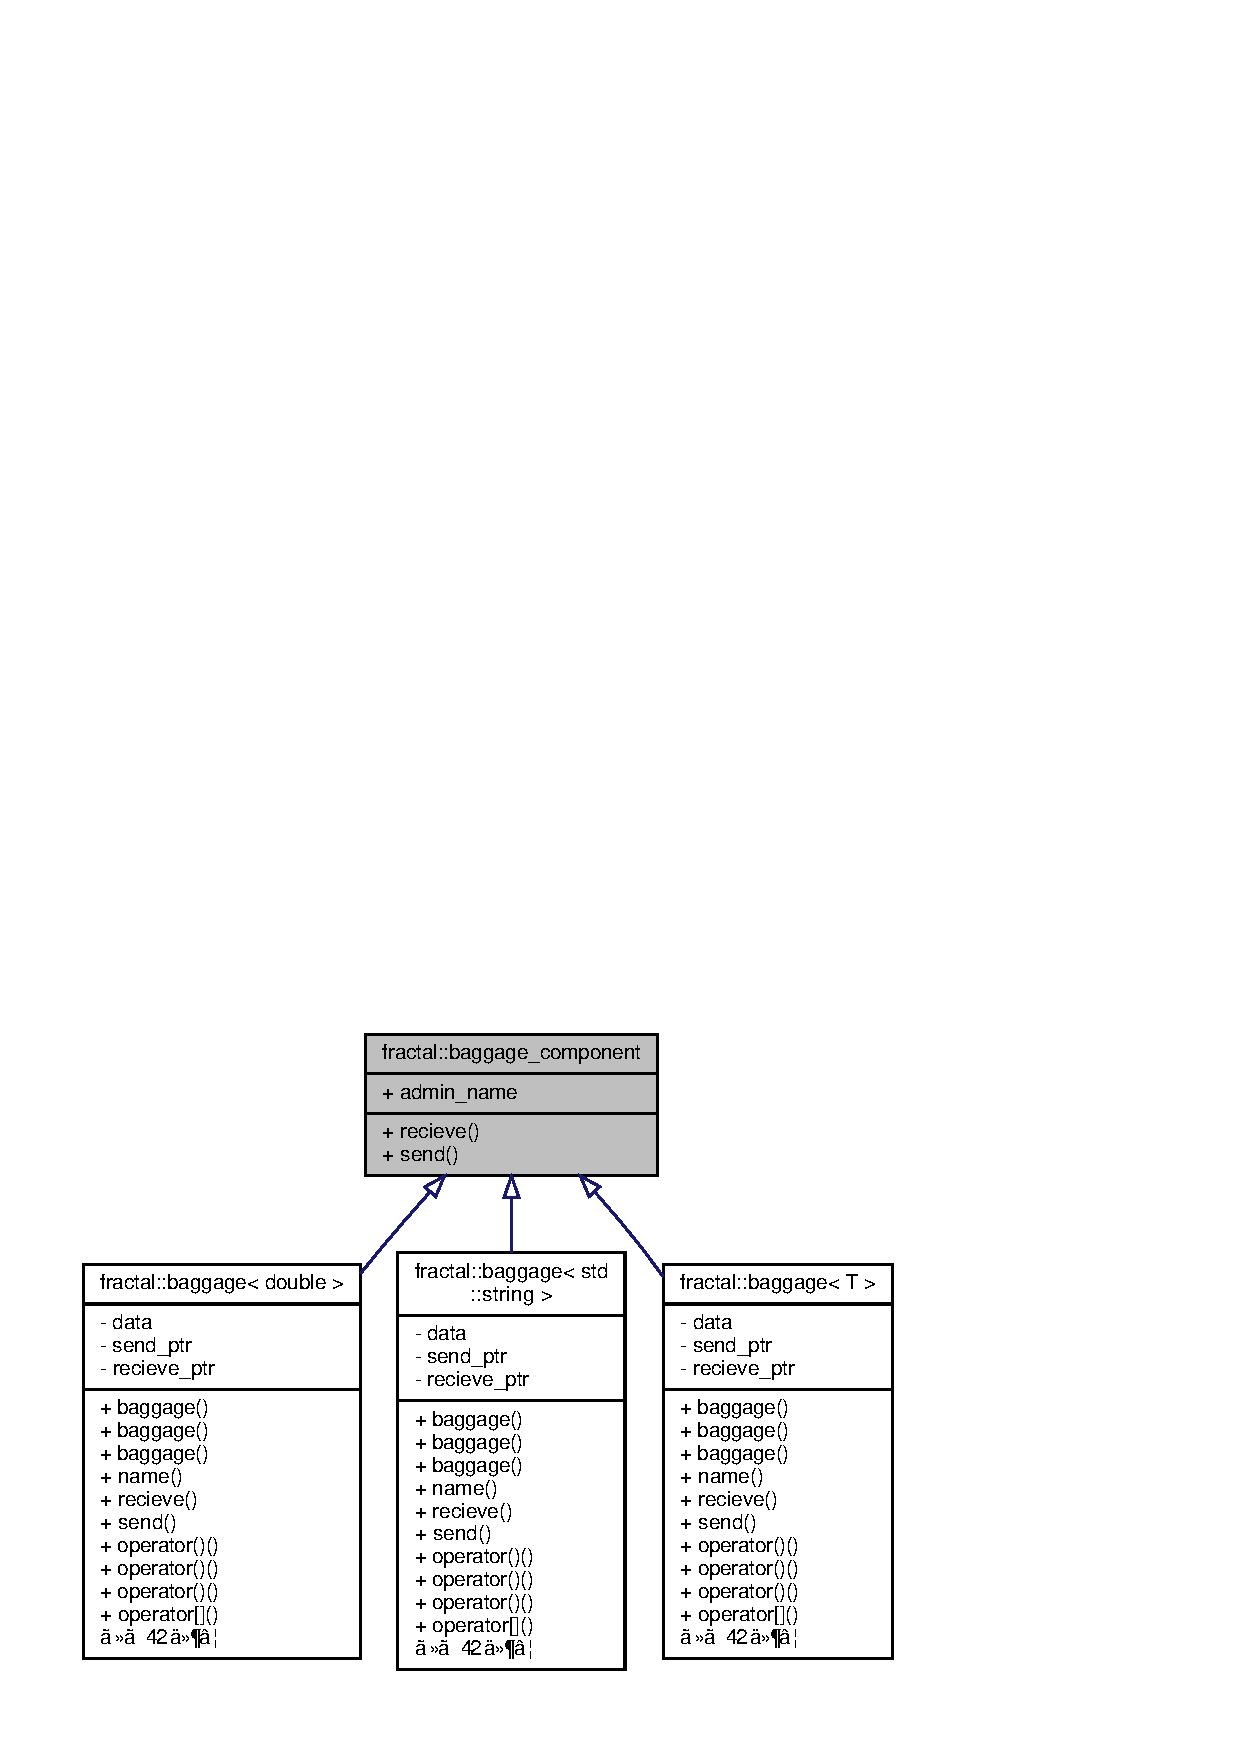
\includegraphics[width=350pt]{classfractal_1_1baggage__component__inherit__graph}
\end{center}
\end{figure}


fractal\+:\+:baggage\+\_\+component 連携図
\nopagebreak
\begin{figure}[H]
\begin{center}
\leavevmode
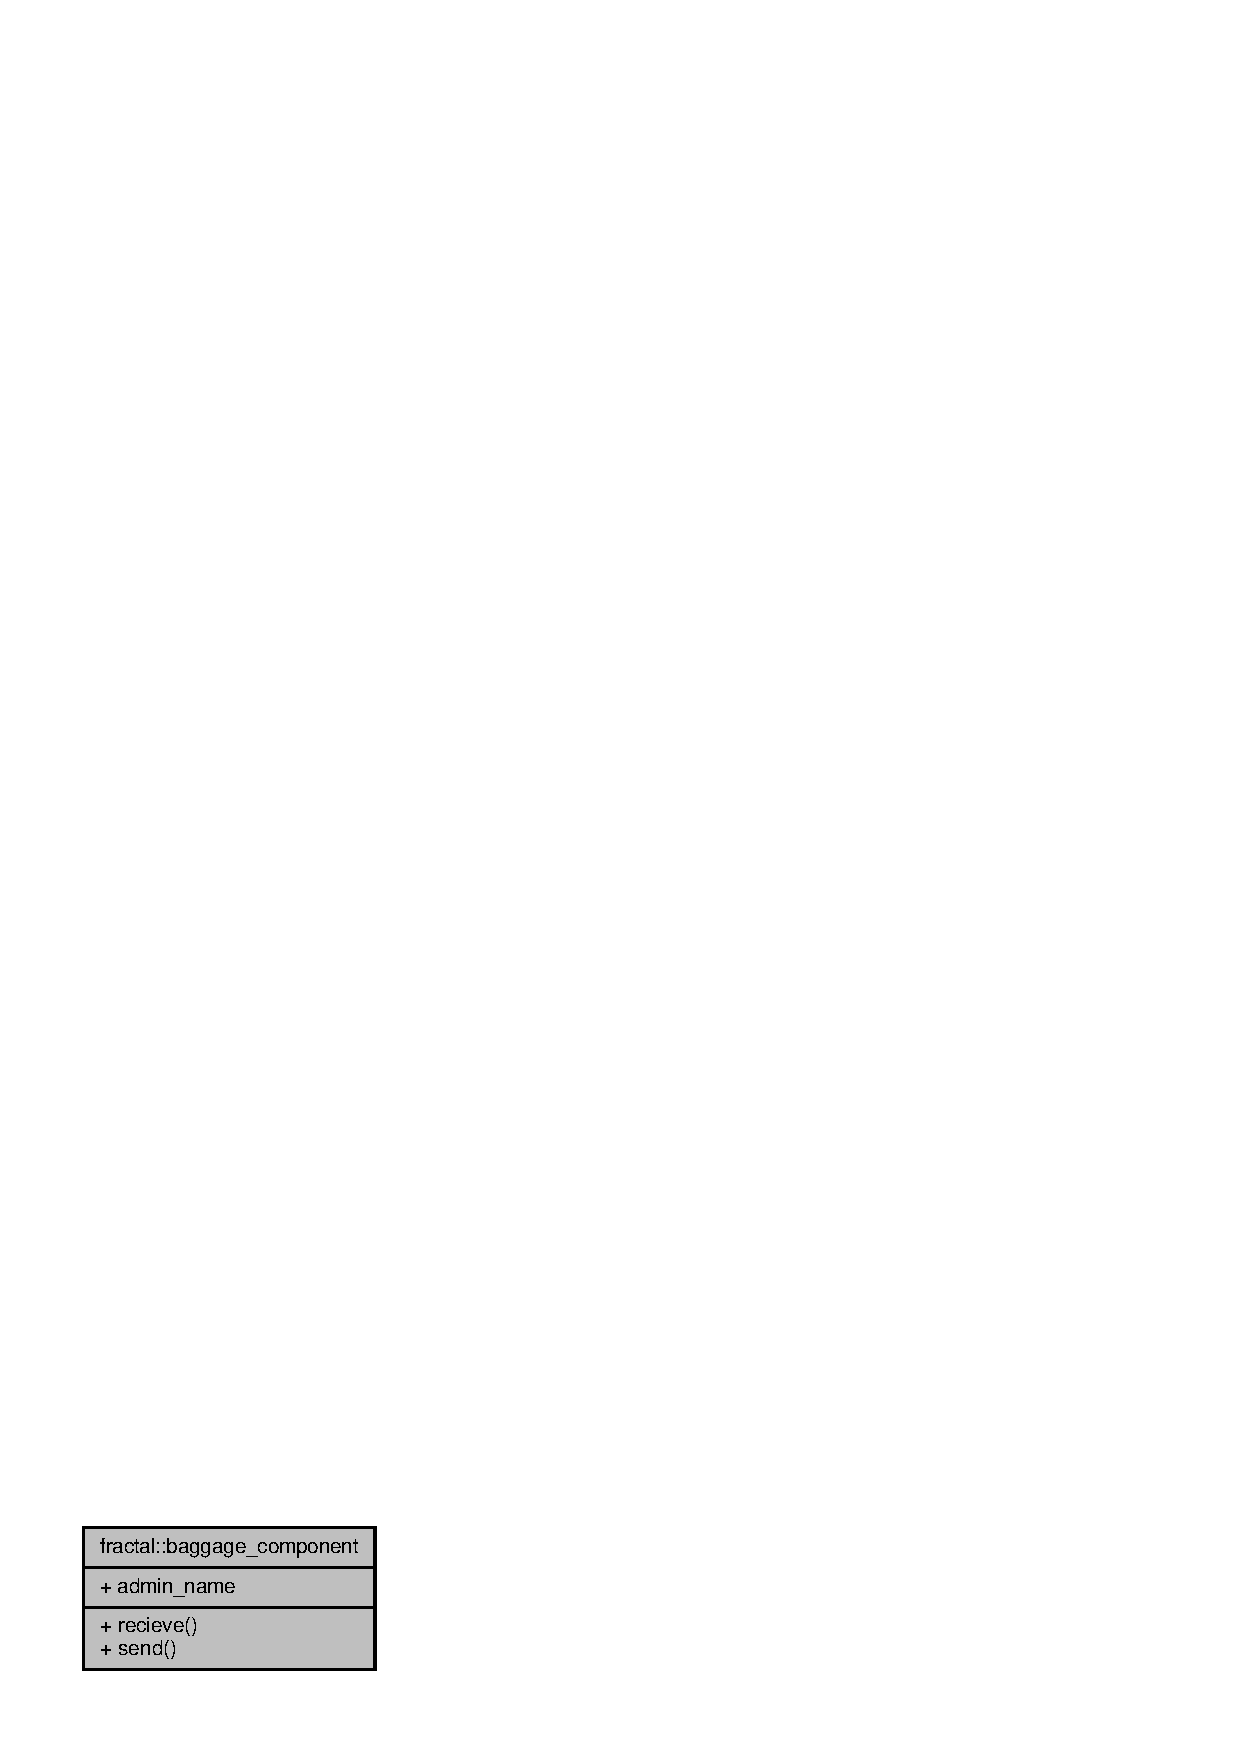
\includegraphics[width=184pt]{classfractal_1_1baggage__component__coll__graph}
\end{center}
\end{figure}
\subsection*{公開メンバ関数}
\begin{DoxyCompactItemize}
\item 
virtual void \hyperlink{classfractal_1_1baggage__component_a37ef357c567ca8844d1b83c83e86df74}{recieve} (void)
\item 
virtual void \hyperlink{classfractal_1_1baggage__component_a8fdf9e534f892911e674de5a60eadf64}{send} (void)
\end{DoxyCompactItemize}
\subsection*{公開変数類}
\begin{DoxyCompactItemize}
\item 
std\+::string \hyperlink{classfractal_1_1baggage__component_a629dba0fbfbce31e2caeb075440ee2dc}{admin\+\_\+name} = \char`\"{}not name\char`\"{}
\begin{DoxyCompactList}\small\item\em admin class name \end{DoxyCompactList}\end{DoxyCompactItemize}


\subsection{関数詳解}
\mbox{\label{classfractal_1_1baggage__component_a37ef357c567ca8844d1b83c83e86df74}} 
\index{fractal\+::baggage\+\_\+component@{fractal\+::baggage\+\_\+component}!recieve@{recieve}}
\index{recieve@{recieve}!fractal\+::baggage\+\_\+component@{fractal\+::baggage\+\_\+component}}
\subsubsection{\texorpdfstring{recieve()}{recieve()}}
{\footnotesize\ttfamily virtual void fractal\+::baggage\+\_\+component\+::recieve (\begin{DoxyParamCaption}\item[{void}]{ }\end{DoxyParamCaption})\hspace{0.3cm}{\ttfamily [inline]}, {\ttfamily [virtual]}}



\hyperlink{classfractal_1_1baggage_aa7d07fc98f7c76789e6047345b2119ce}{fractal\+::baggage$<$ T $>$}, \hyperlink{classfractal_1_1baggage_aa7d07fc98f7c76789e6047345b2119ce}{fractal\+::baggage$<$ double $>$}, \hyperlink{classfractal_1_1baggage_aa7d07fc98f7c76789e6047345b2119ce}{fractal\+::baggage$<$ std\+::string $>$}で再実装されています。

被呼び出し関係図\+:
\nopagebreak
\begin{figure}[H]
\begin{center}
\leavevmode
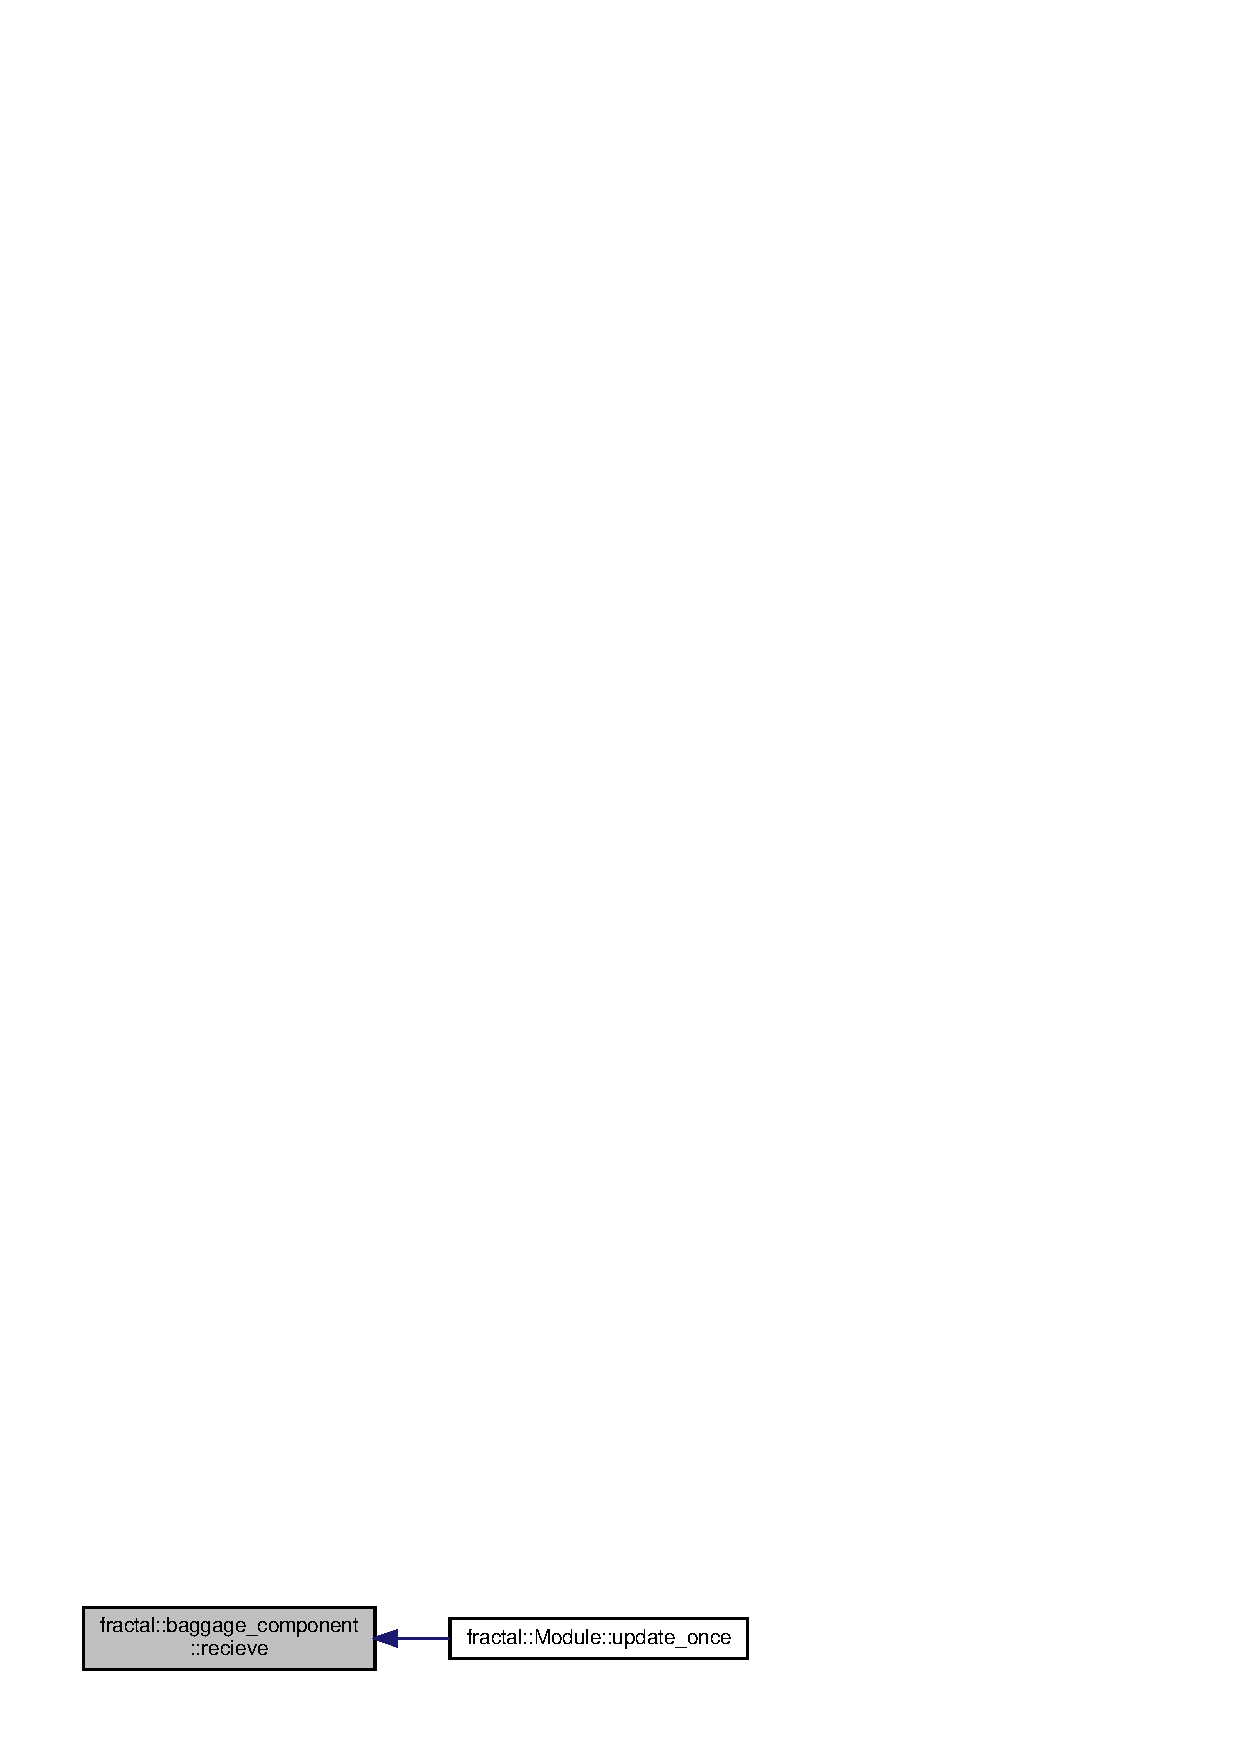
\includegraphics[width=350pt]{classfractal_1_1baggage__component_a37ef357c567ca8844d1b83c83e86df74_icgraph}
\end{center}
\end{figure}
\mbox{\label{classfractal_1_1baggage__component_a8fdf9e534f892911e674de5a60eadf64}} 
\index{fractal\+::baggage\+\_\+component@{fractal\+::baggage\+\_\+component}!send@{send}}
\index{send@{send}!fractal\+::baggage\+\_\+component@{fractal\+::baggage\+\_\+component}}
\subsubsection{\texorpdfstring{send()}{send()}}
{\footnotesize\ttfamily virtual void fractal\+::baggage\+\_\+component\+::send (\begin{DoxyParamCaption}\item[{void}]{ }\end{DoxyParamCaption})\hspace{0.3cm}{\ttfamily [inline]}, {\ttfamily [virtual]}}



\hyperlink{classfractal_1_1baggage_a12ef96c1b906369cfeeabdead61c257b}{fractal\+::baggage$<$ T $>$}, \hyperlink{classfractal_1_1baggage_a12ef96c1b906369cfeeabdead61c257b}{fractal\+::baggage$<$ double $>$}, \hyperlink{classfractal_1_1baggage_a12ef96c1b906369cfeeabdead61c257b}{fractal\+::baggage$<$ std\+::string $>$}で再実装されています。

被呼び出し関係図\+:
\nopagebreak
\begin{figure}[H]
\begin{center}
\leavevmode
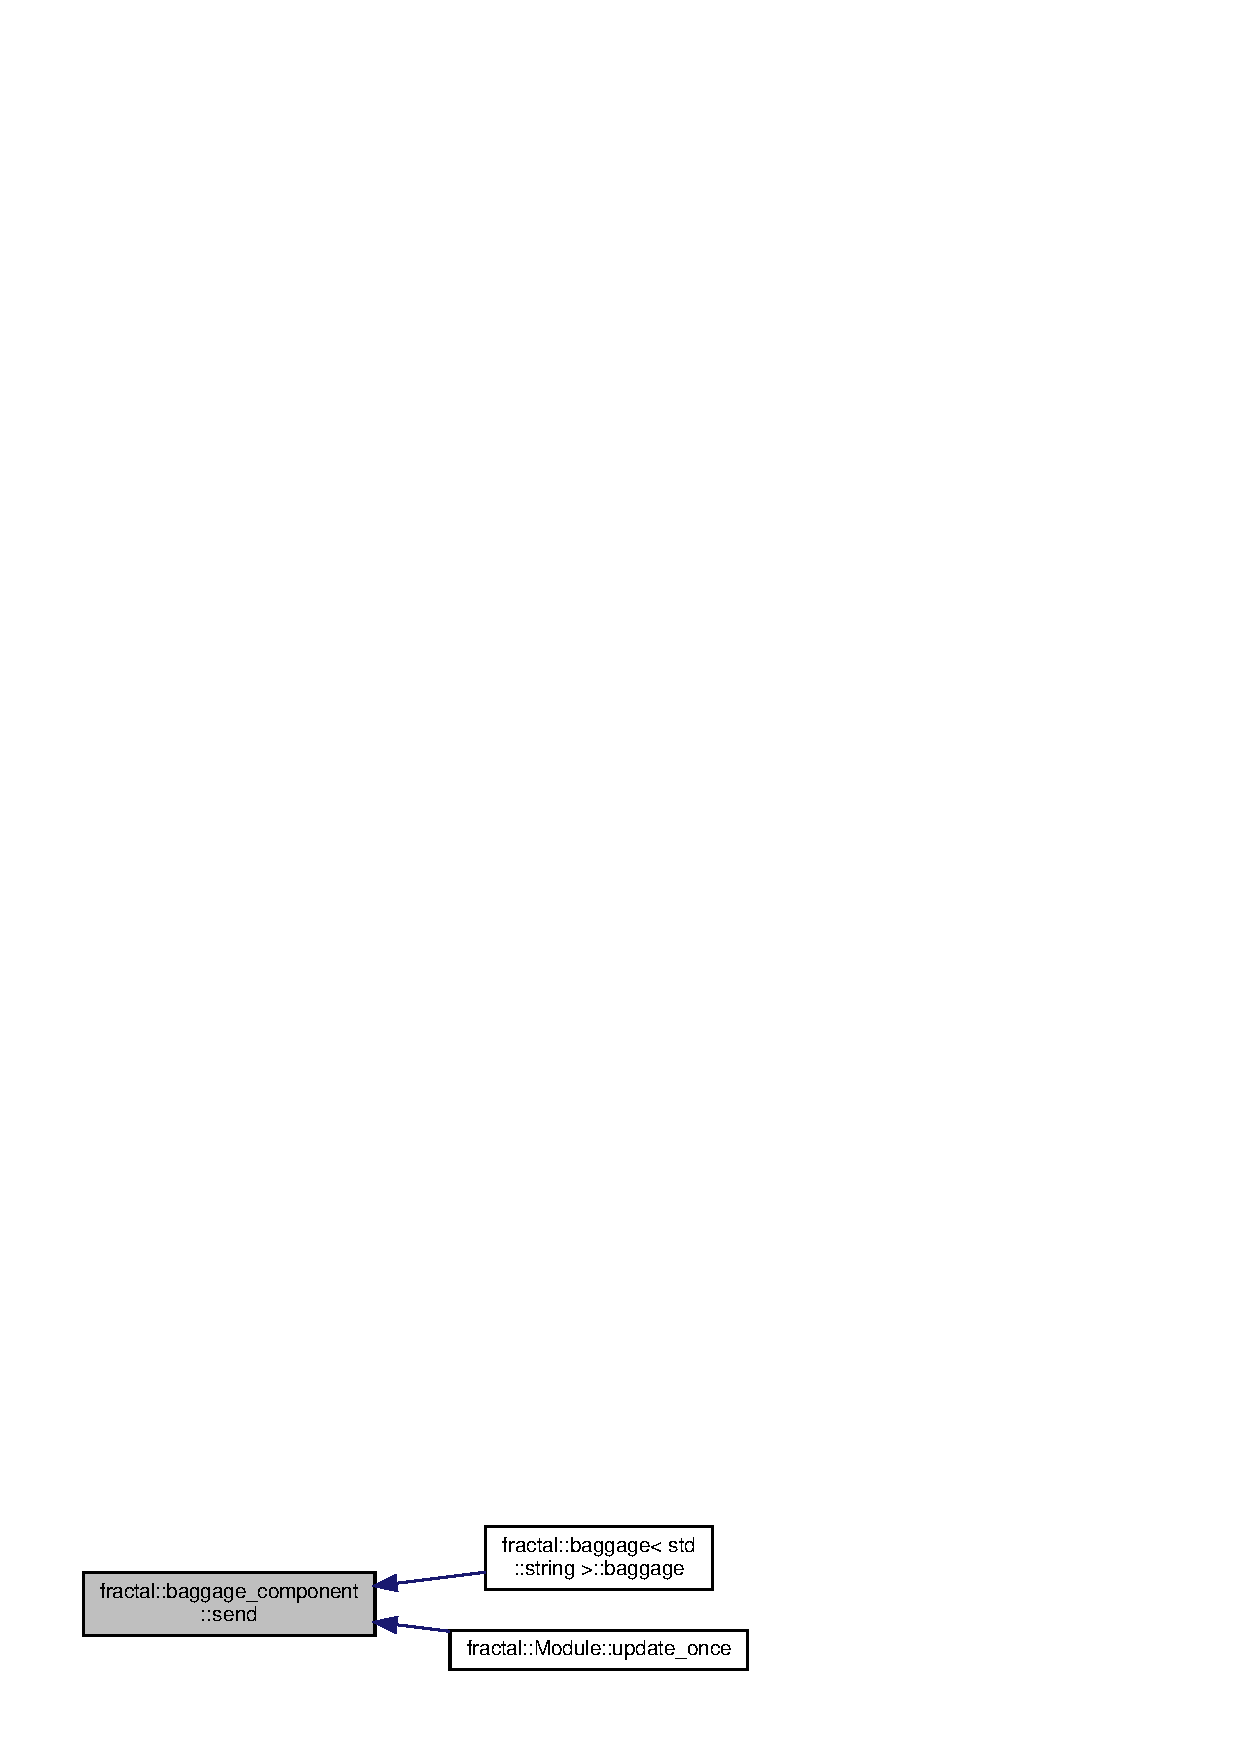
\includegraphics[width=350pt]{classfractal_1_1baggage__component_a8fdf9e534f892911e674de5a60eadf64_icgraph}
\end{center}
\end{figure}


\subsection{メンバ詳解}
\mbox{\label{classfractal_1_1baggage__component_a629dba0fbfbce31e2caeb075440ee2dc}} 
\index{fractal\+::baggage\+\_\+component@{fractal\+::baggage\+\_\+component}!admin\+\_\+name@{admin\+\_\+name}}
\index{admin\+\_\+name@{admin\+\_\+name}!fractal\+::baggage\+\_\+component@{fractal\+::baggage\+\_\+component}}
\subsubsection{\texorpdfstring{admin\+\_\+name}{admin\_name}}
{\footnotesize\ttfamily std\+::string fractal\+::baggage\+\_\+component\+::admin\+\_\+name = \char`\"{}not name\char`\"{}}



admin class name 



このクラス詳解は次のファイルから抽出されました\+:\begin{DoxyCompactItemize}
\item 
/home/takanobu/fractal/include/\hyperlink{fractal_8h}{fractal.\+h}\end{DoxyCompactItemize}

\section{fractal\+:\+:Dummy クラス}
\label{classfractal_1_1Dummy}\index{fractal\+::\+Dummy@{fractal\+::\+Dummy}}


Empty Class  




{\ttfamily \#include $<$fractal.\+h$>$}



fractal\+:\+:Dummy 連携図
\nopagebreak
\begin{figure}[H]
\begin{center}
\leavevmode
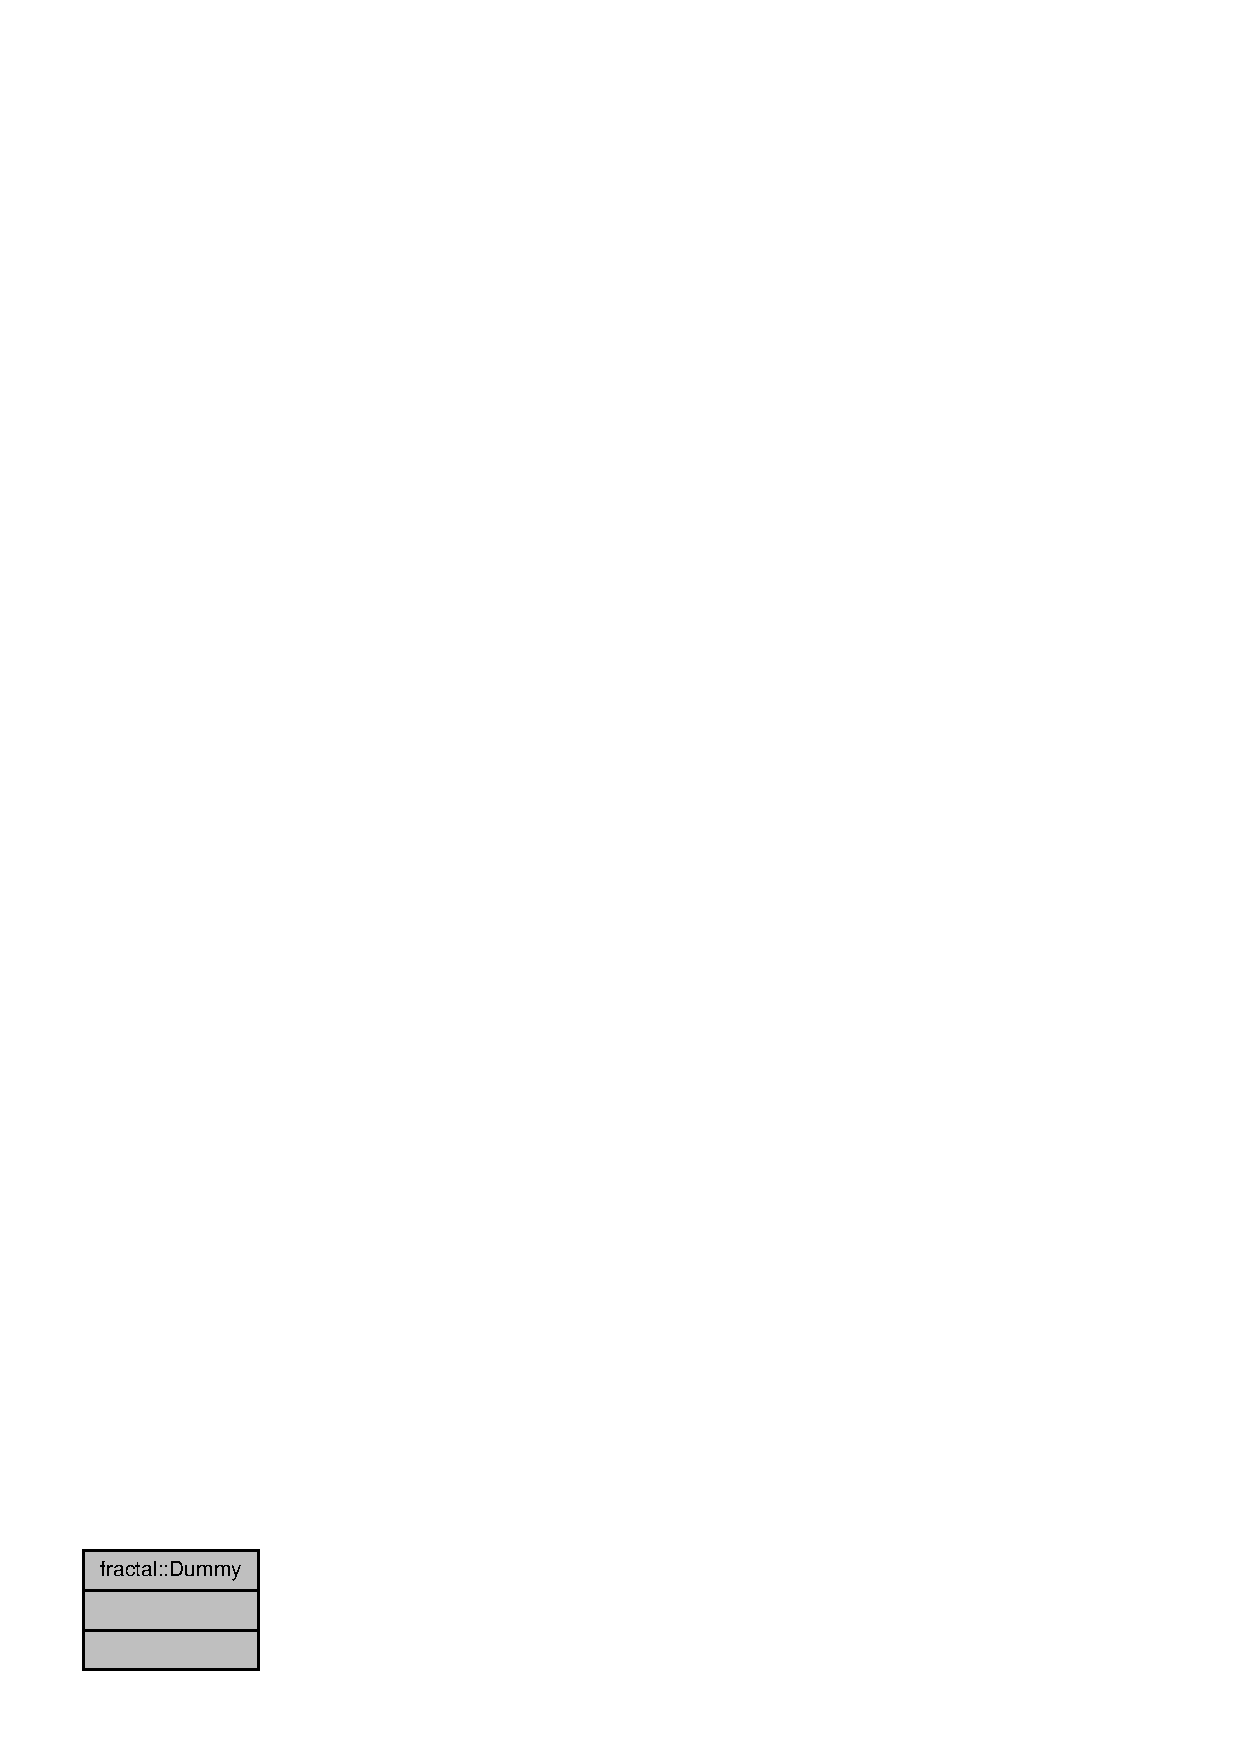
\includegraphics[width=128pt]{classfractal_1_1Dummy__coll__graph}
\end{center}
\end{figure}


\subsection{詳解}
Empty Class 

this class is dummy 

このクラス詳解は次のファイルから抽出されました\+:\begin{DoxyCompactItemize}
\item 
/home/takanobu/fractal/include/\hyperlink{fractal_8h}{fractal.\+h}\end{DoxyCompactItemize}

\section{fractal\+:\+:Module クラス}
\label{classfractal_1_1Module}\index{fractal\+::\+Module@{fractal\+::\+Module}}


\hyperlink{classfractal_1_1Module}{Module} Class  




{\ttfamily \#include $<$fractal.\+h$>$}



fractal\+:\+:Module の継承関係図
\nopagebreak
\begin{figure}[H]
\begin{center}
\leavevmode
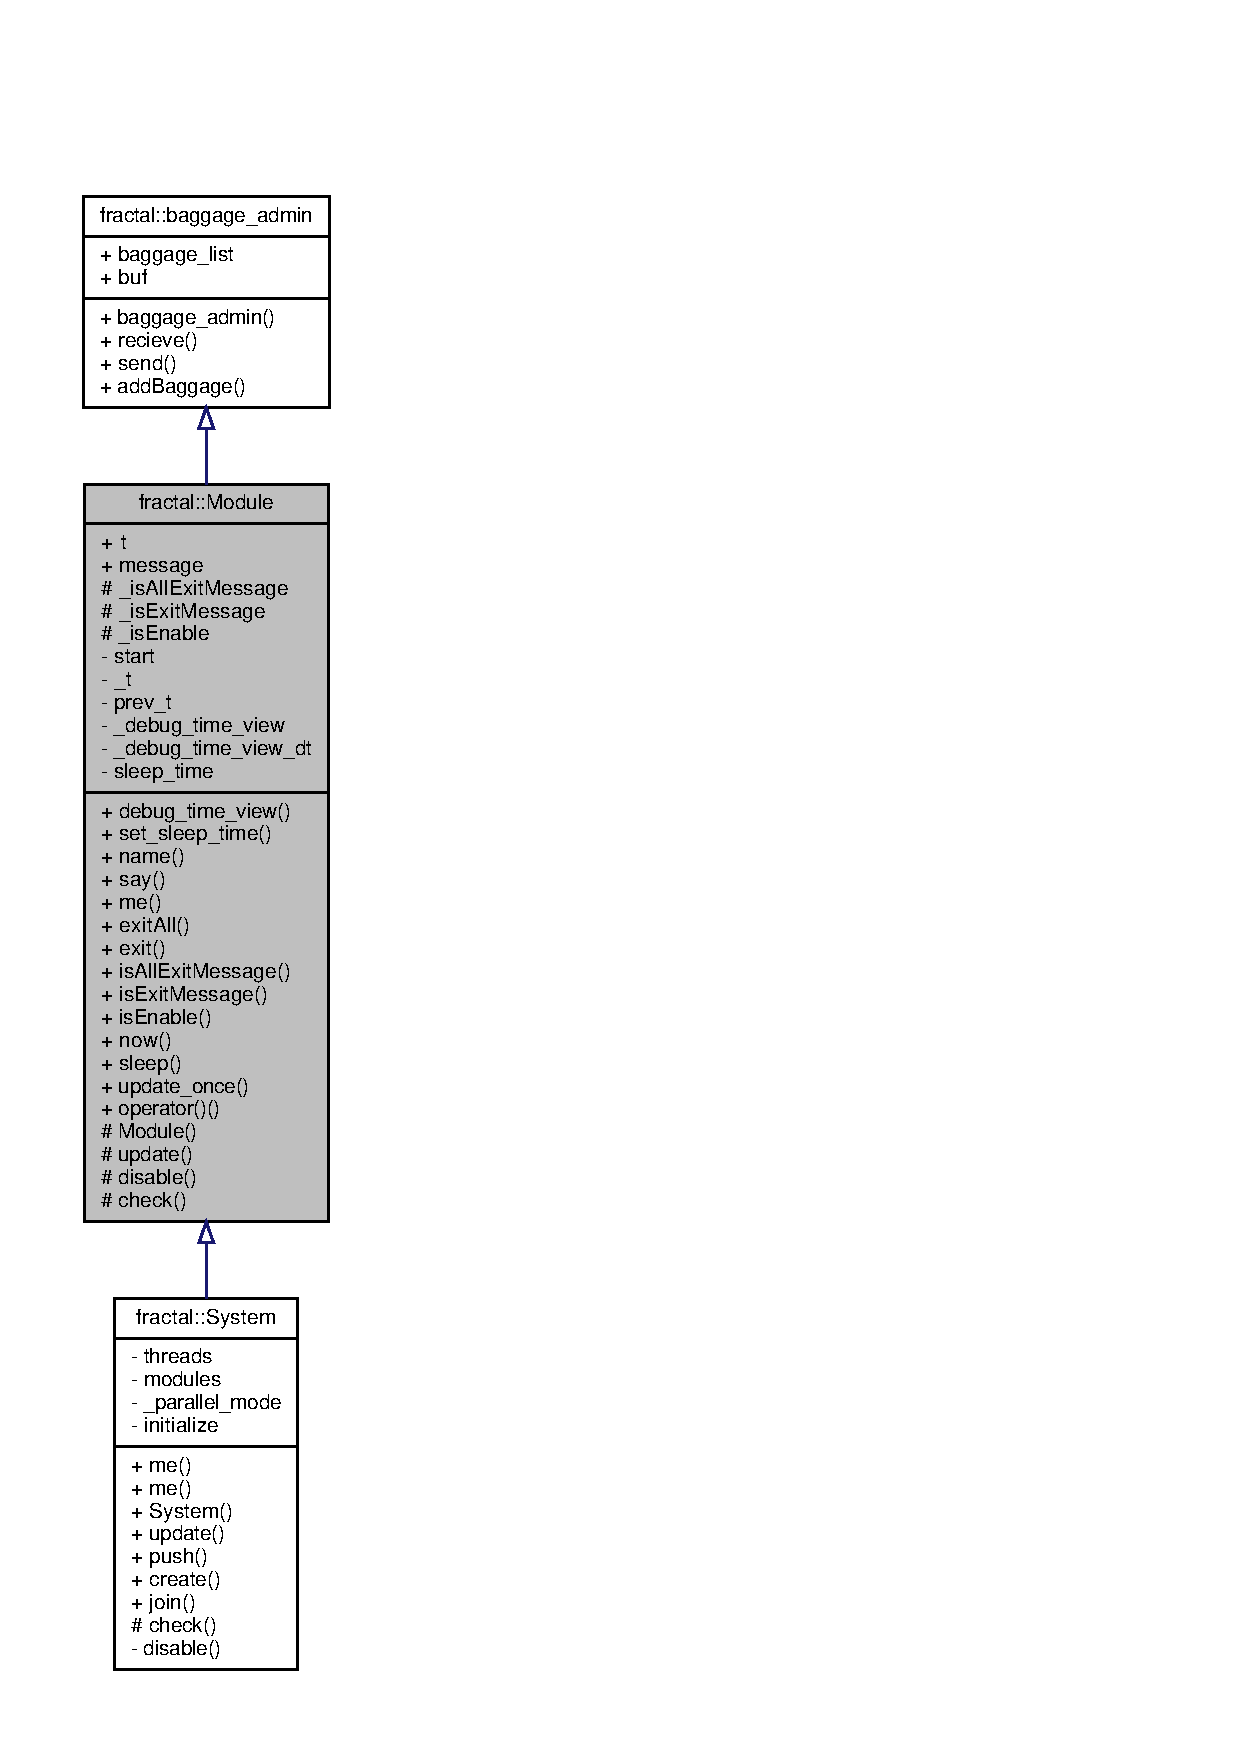
\includegraphics[height=550pt]{classfractal_1_1Module__inherit__graph}
\end{center}
\end{figure}


fractal\+:\+:Module 連携図
\nopagebreak
\begin{figure}[H]
\begin{center}
\leavevmode
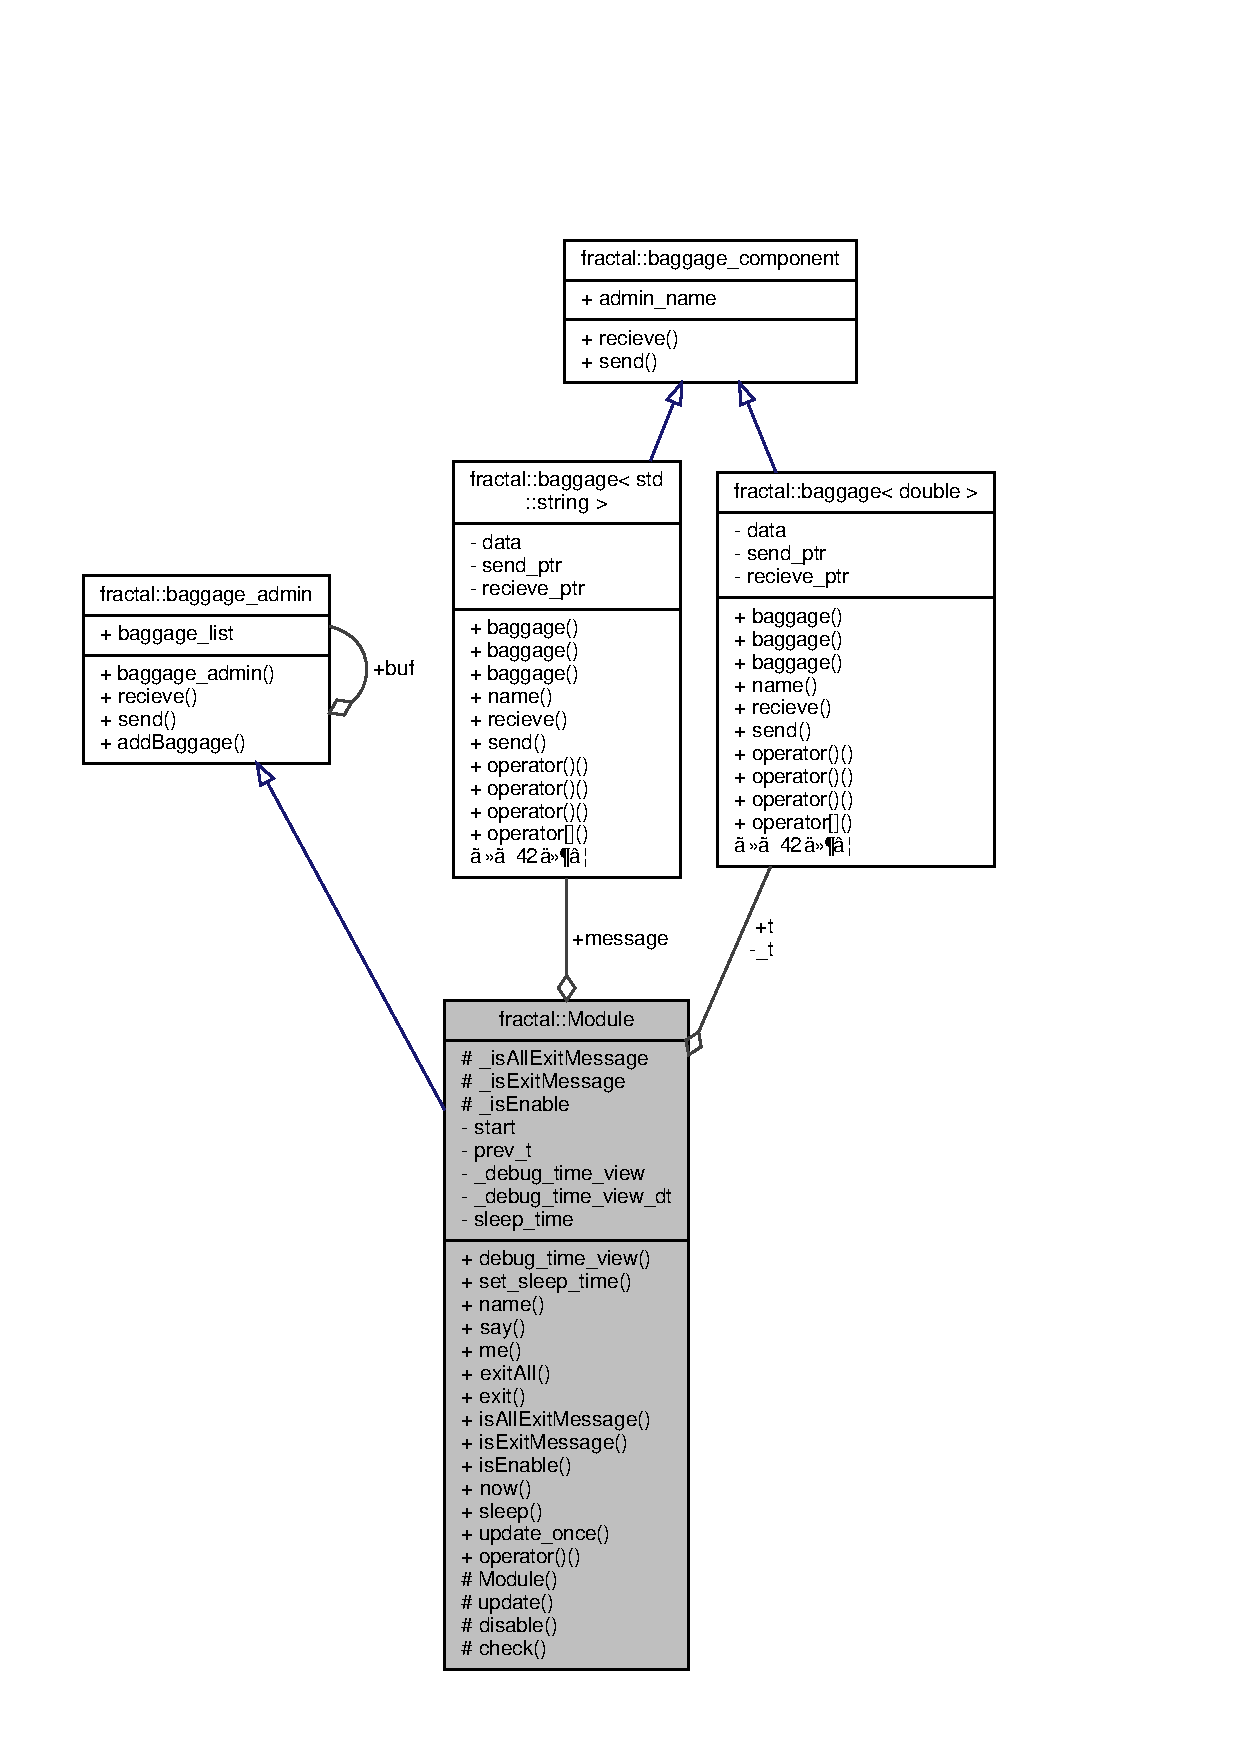
\includegraphics[width=350pt]{classfractal_1_1Module__coll__graph}
\end{center}
\end{figure}
\subsection*{公開メンバ関数}
\begin{DoxyCompactItemize}
\item 
void \hyperlink{classfractal_1_1Module_aa1799cce209611e46fafb8e826f4dc2e}{debug\+\_\+time\+\_\+view} (double dt)
\item 
void \hyperlink{classfractal_1_1Module_a4cd49e1c42043ea4254a8859992f5a64}{set\+\_\+sleep\+\_\+time} (double dt)
\item 
std\+::string \hyperlink{classfractal_1_1Module_a770fab9c6a6f310e76a9c29ed9c7d515}{name} (void)
\begin{DoxyCompactList}\small\item\em get class name of myself \end{DoxyCompactList}\item 
virtual void \hyperlink{classfractal_1_1Module_afd605b7a7ef55d5d0a55f520ff8feb86}{say} (std\+::string str)
\begin{DoxyCompactList}\small\item\em standard output any string \end{DoxyCompactList}\item 
virtual void \hyperlink{classfractal_1_1Module_a92deaafb88a2bc34958dca99fdc112a3}{me} (int n)
\begin{DoxyCompactList}\small\item\em show class name \end{DoxyCompactList}\item 
void \hyperlink{classfractal_1_1Module_a40cfc2e5ab9829d5decaef0ce30cdbcc}{exit\+All} (void)
\begin{DoxyCompactList}\small\item\em exit all modules \end{DoxyCompactList}\item 
void \hyperlink{classfractal_1_1Module_a04ba8c14e82f92c1db411662d7a16cd8}{exit} (void)
\begin{DoxyCompactList}\small\item\em exit this module \end{DoxyCompactList}\item 
bool \hyperlink{classfractal_1_1Module_a7766711ae2e854ee7a723781ef1b2572}{is\+All\+Exit\+Message} (void)
\begin{DoxyCompactList}\small\item\em exit flag for all modules  true if there is exit message \end{DoxyCompactList}\item 
bool \hyperlink{classfractal_1_1Module_a9b79e3353f502cb49f7bb713266ebdef}{is\+Exit\+Message} (void)
\begin{DoxyCompactList}\small\item\em exit flag for this module  true if there is exit message \end{DoxyCompactList}\item 
bool \hyperlink{classfractal_1_1Module_a74c4dc6f8d5f57d885b0da633ec12e1f}{is\+Enable} (void)
\begin{DoxyCompactList}\small\item\em status of this module  true if this module is enable \end{DoxyCompactList}\item 
std\+::chrono\+::system\+\_\+clock\+::time\+\_\+point \hyperlink{classfractal_1_1Module_a4618e1597d01313ffb69116ed3dcdbfa}{now} (void)
\item 
void \hyperlink{classfractal_1_1Module_aba781b23b4f5ae00609f1daee3a0072c}{sleep} (double dt)
\item 
void \hyperlink{classfractal_1_1Module_abc2bf9795de848ecef0bd2e339a81e0d}{update\+\_\+once} (bool parallel\+\_\+mode=false)
\item 
void \hyperlink{classfractal_1_1Module_ae738b02bc66ce9aaf425902bd01b9503}{operator()} (void)
\end{DoxyCompactItemize}
\subsection*{公開変数類}
\begin{DoxyCompactItemize}
\item 
\hyperlink{classfractal_1_1baggage}{baggage}$<$ double $>$ \hyperlink{classfractal_1_1Module_ac14a8d440a0a4f7a0be952a902c3717e}{t} = 0
\begin{DoxyCompactList}\small\item\em synchronization time \end{DoxyCompactList}\item 
\hyperlink{classfractal_1_1baggage}{baggage}$<$ std\+::string $>$ \hyperlink{classfractal_1_1Module_a8e59ac0be2426bde4e79a589ffc4cce4}{message}
\begin{DoxyCompactList}\small\item\em message \end{DoxyCompactList}\end{DoxyCompactItemize}
\subsection*{限定公開メンバ関数}
\begin{DoxyCompactItemize}
\item 
\hyperlink{classfractal_1_1Module_a43c2b0b93b603ee601af3c90931ff7f6}{Module} (void)
\item 
virtual void \hyperlink{classfractal_1_1Module_ad68342ebc960bb0e1dd19b7c70bc3753}{update} (double dt)
\begin{DoxyCompactList}\small\item\em update function \end{DoxyCompactList}\item 
virtual void \hyperlink{classfractal_1_1Module_a17a7773769fb523fd4b2aeb28366debe}{disable} (void)
\begin{DoxyCompactList}\small\item\em  disable this module \end{DoxyCompactList}\item 
virtual void \hyperlink{classfractal_1_1Module_a245865f346ac1d21b19bce418bf704c4}{check} (void)
\begin{DoxyCompactList}\small\item\em check exit message \end{DoxyCompactList}\end{DoxyCompactItemize}
\subsection*{限定公開変数類}
\begin{DoxyCompactItemize}
\item 
bool \hyperlink{classfractal_1_1Module_aed6038d7f13a217f171c3fa1a29e7129}{\+\_\+is\+All\+Exit\+Message} = false
\begin{DoxyCompactList}\small\item\em exit flag for all modules \end{DoxyCompactList}\item 
bool \hyperlink{classfractal_1_1Module_a3c0219468a7d043c70420cca57f39989}{\+\_\+is\+Exit\+Message} = false
\begin{DoxyCompactList}\small\item\em exit flag for this modules \end{DoxyCompactList}\item 
bool \hyperlink{classfractal_1_1Module_ac1194f7c1723026348f7dc2df099ccf6}{\+\_\+is\+Enable} = true
\begin{DoxyCompactList}\small\item\em status of this module \end{DoxyCompactList}\end{DoxyCompactItemize}
\subsection*{非公開変数類}
\begin{DoxyCompactItemize}
\item 
std\+::chrono\+::system\+\_\+clock\+::time\+\_\+point \hyperlink{classfractal_1_1Module_a869fe7b6421f11439ac696867a71d9eb}{start}
\item 
\hyperlink{classfractal_1_1baggage}{baggage}$<$ double $>$ \hyperlink{classfractal_1_1Module_a36d598812541ddb73bb733dbcd708974}{\+\_\+t} = 0
\begin{DoxyCompactList}\small\item\em internal time \end{DoxyCompactList}\item 
double \hyperlink{classfractal_1_1Module_a47a4704bcfc9255a2e2ee8c81676a9f8}{prev\+\_\+t} = 0
\item 
bool \hyperlink{classfractal_1_1Module_a10311e3d5bff39ed0facbfe3b0eb9f0d}{\+\_\+debug\+\_\+time\+\_\+view} = false
\item 
double \hyperlink{classfractal_1_1Module_adb17cd3c5a3edc29e0716d0f7abde9e8}{\+\_\+debug\+\_\+time\+\_\+view\+\_\+dt} = 0.\+0
\item 
double \hyperlink{classfractal_1_1Module_a8f01c07a782ebc8bbdab28212e275979}{sleep\+\_\+time} = 0.\+0005
\end{DoxyCompactItemize}
\subsection*{その他の継承メンバ}


\subsection{詳解}
\hyperlink{classfractal_1_1Module}{Module} Class 

base class for modules 

\subsection{構築子と解体子}
\mbox{\label{classfractal_1_1Module_a43c2b0b93b603ee601af3c90931ff7f6}} 
\index{fractal\+::\+Module@{fractal\+::\+Module}!Module@{Module}}
\index{Module@{Module}!fractal\+::\+Module@{fractal\+::\+Module}}
\subsubsection{\texorpdfstring{Module()}{Module()}}
{\footnotesize\ttfamily fractal\+::\+Module\+::\+Module (\begin{DoxyParamCaption}\item[{void}]{ }\end{DoxyParamCaption})\hspace{0.3cm}{\ttfamily [inline]}, {\ttfamily [protected]}}



\subsection{関数詳解}
\mbox{\label{classfractal_1_1Module_a245865f346ac1d21b19bce418bf704c4}} 
\index{fractal\+::\+Module@{fractal\+::\+Module}!check@{check}}
\index{check@{check}!fractal\+::\+Module@{fractal\+::\+Module}}
\subsubsection{\texorpdfstring{check()}{check()}}
{\footnotesize\ttfamily virtual void fractal\+::\+Module\+::check (\begin{DoxyParamCaption}\item[{void}]{ }\end{DoxyParamCaption})\hspace{0.3cm}{\ttfamily [inline]}, {\ttfamily [protected]}, {\ttfamily [virtual]}}



check exit message 



\hyperlink{classfractal_1_1System_a95f99e9132a10f87f9179a27c840fa50}{fractal\+::\+System}で再実装されています。

\mbox{\label{classfractal_1_1Module_aa1799cce209611e46fafb8e826f4dc2e}} 
\index{fractal\+::\+Module@{fractal\+::\+Module}!debug\+\_\+time\+\_\+view@{debug\+\_\+time\+\_\+view}}
\index{debug\+\_\+time\+\_\+view@{debug\+\_\+time\+\_\+view}!fractal\+::\+Module@{fractal\+::\+Module}}
\subsubsection{\texorpdfstring{debug\+\_\+time\+\_\+view()}{debug\_time\_view()}}
{\footnotesize\ttfamily void fractal\+::\+Module\+::debug\+\_\+time\+\_\+view (\begin{DoxyParamCaption}\item[{double}]{dt }\end{DoxyParamCaption})\hspace{0.3cm}{\ttfamily [inline]}}

\mbox{\label{classfractal_1_1Module_a17a7773769fb523fd4b2aeb28366debe}} 
\index{fractal\+::\+Module@{fractal\+::\+Module}!disable@{disable}}
\index{disable@{disable}!fractal\+::\+Module@{fractal\+::\+Module}}
\subsubsection{\texorpdfstring{disable()}{disable()}}
{\footnotesize\ttfamily virtual void fractal\+::\+Module\+::disable (\begin{DoxyParamCaption}\item[{void}]{ }\end{DoxyParamCaption})\hspace{0.3cm}{\ttfamily [inline]}, {\ttfamily [protected]}, {\ttfamily [virtual]}}



 disable this module 



\hyperlink{classfractal_1_1System_a446532d4c3811f6005e0c52ad653a997}{fractal\+::\+System}で再実装されています。

\mbox{\label{classfractal_1_1Module_a04ba8c14e82f92c1db411662d7a16cd8}} 
\index{fractal\+::\+Module@{fractal\+::\+Module}!exit@{exit}}
\index{exit@{exit}!fractal\+::\+Module@{fractal\+::\+Module}}
\subsubsection{\texorpdfstring{exit()}{exit()}}
{\footnotesize\ttfamily void fractal\+::\+Module\+::exit (\begin{DoxyParamCaption}\item[{void}]{ }\end{DoxyParamCaption})\hspace{0.3cm}{\ttfamily [inline]}}



exit this module 

\mbox{\label{classfractal_1_1Module_a40cfc2e5ab9829d5decaef0ce30cdbcc}} 
\index{fractal\+::\+Module@{fractal\+::\+Module}!exit\+All@{exit\+All}}
\index{exit\+All@{exit\+All}!fractal\+::\+Module@{fractal\+::\+Module}}
\subsubsection{\texorpdfstring{exit\+All()}{exitAll()}}
{\footnotesize\ttfamily void fractal\+::\+Module\+::exit\+All (\begin{DoxyParamCaption}\item[{void}]{ }\end{DoxyParamCaption})\hspace{0.3cm}{\ttfamily [inline]}}



exit all modules 

\mbox{\label{classfractal_1_1Module_a7766711ae2e854ee7a723781ef1b2572}} 
\index{fractal\+::\+Module@{fractal\+::\+Module}!is\+All\+Exit\+Message@{is\+All\+Exit\+Message}}
\index{is\+All\+Exit\+Message@{is\+All\+Exit\+Message}!fractal\+::\+Module@{fractal\+::\+Module}}
\subsubsection{\texorpdfstring{is\+All\+Exit\+Message()}{isAllExitMessage()}}
{\footnotesize\ttfamily bool fractal\+::\+Module\+::is\+All\+Exit\+Message (\begin{DoxyParamCaption}\item[{void}]{ }\end{DoxyParamCaption})\hspace{0.3cm}{\ttfamily [inline]}}



exit flag for all modules  true if there is exit message 

\mbox{\label{classfractal_1_1Module_a74c4dc6f8d5f57d885b0da633ec12e1f}} 
\index{fractal\+::\+Module@{fractal\+::\+Module}!is\+Enable@{is\+Enable}}
\index{is\+Enable@{is\+Enable}!fractal\+::\+Module@{fractal\+::\+Module}}
\subsubsection{\texorpdfstring{is\+Enable()}{isEnable()}}
{\footnotesize\ttfamily bool fractal\+::\+Module\+::is\+Enable (\begin{DoxyParamCaption}\item[{void}]{ }\end{DoxyParamCaption})\hspace{0.3cm}{\ttfamily [inline]}}



status of this module  true if this module is enable 

\mbox{\label{classfractal_1_1Module_a9b79e3353f502cb49f7bb713266ebdef}} 
\index{fractal\+::\+Module@{fractal\+::\+Module}!is\+Exit\+Message@{is\+Exit\+Message}}
\index{is\+Exit\+Message@{is\+Exit\+Message}!fractal\+::\+Module@{fractal\+::\+Module}}
\subsubsection{\texorpdfstring{is\+Exit\+Message()}{isExitMessage()}}
{\footnotesize\ttfamily bool fractal\+::\+Module\+::is\+Exit\+Message (\begin{DoxyParamCaption}\item[{void}]{ }\end{DoxyParamCaption})\hspace{0.3cm}{\ttfamily [inline]}}



exit flag for this module  true if there is exit message 

\mbox{\label{classfractal_1_1Module_a92deaafb88a2bc34958dca99fdc112a3}} 
\index{fractal\+::\+Module@{fractal\+::\+Module}!me@{me}}
\index{me@{me}!fractal\+::\+Module@{fractal\+::\+Module}}
\subsubsection{\texorpdfstring{me()}{me()}}
{\footnotesize\ttfamily virtual void fractal\+::\+Module\+::me (\begin{DoxyParamCaption}\item[{int}]{n }\end{DoxyParamCaption})\hspace{0.3cm}{\ttfamily [inline]}, {\ttfamily [virtual]}}



show class name 


\begin{DoxyParams}{引数}
{\em n} & layer number \\
\hline
\end{DoxyParams}


\hyperlink{classfractal_1_1System_aa8e8768417ccfe745def786d63eee80d}{fractal\+::\+System}で再実装されています。

\mbox{\label{classfractal_1_1Module_a770fab9c6a6f310e76a9c29ed9c7d515}} 
\index{fractal\+::\+Module@{fractal\+::\+Module}!name@{name}}
\index{name@{name}!fractal\+::\+Module@{fractal\+::\+Module}}
\subsubsection{\texorpdfstring{name()}{name()}}
{\footnotesize\ttfamily std\+::string fractal\+::\+Module\+::name (\begin{DoxyParamCaption}\item[{void}]{ }\end{DoxyParamCaption})\hspace{0.3cm}{\ttfamily [inline]}}



get class name of myself 

\begin{DoxyReturn}{戻り値}
class name 
\end{DoxyReturn}
\mbox{\label{classfractal_1_1Module_a4618e1597d01313ffb69116ed3dcdbfa}} 
\index{fractal\+::\+Module@{fractal\+::\+Module}!now@{now}}
\index{now@{now}!fractal\+::\+Module@{fractal\+::\+Module}}
\subsubsection{\texorpdfstring{now()}{now()}}
{\footnotesize\ttfamily std\+::chrono\+::system\+\_\+clock\+::time\+\_\+point fractal\+::\+Module\+::now (\begin{DoxyParamCaption}\item[{void}]{ }\end{DoxyParamCaption})\hspace{0.3cm}{\ttfamily [inline]}}

\mbox{\label{classfractal_1_1Module_ae738b02bc66ce9aaf425902bd01b9503}} 
\index{fractal\+::\+Module@{fractal\+::\+Module}!operator()@{operator()}}
\index{operator()@{operator()}!fractal\+::\+Module@{fractal\+::\+Module}}
\subsubsection{\texorpdfstring{operator()()}{operator()()}}
{\footnotesize\ttfamily void fractal\+::\+Module\+::operator() (\begin{DoxyParamCaption}\item[{void}]{ }\end{DoxyParamCaption})\hspace{0.3cm}{\ttfamily [inline]}}

\mbox{\label{classfractal_1_1Module_afd605b7a7ef55d5d0a55f520ff8feb86}} 
\index{fractal\+::\+Module@{fractal\+::\+Module}!say@{say}}
\index{say@{say}!fractal\+::\+Module@{fractal\+::\+Module}}
\subsubsection{\texorpdfstring{say()}{say()}}
{\footnotesize\ttfamily virtual void fractal\+::\+Module\+::say (\begin{DoxyParamCaption}\item[{std\+::string}]{str }\end{DoxyParamCaption})\hspace{0.3cm}{\ttfamily [inline]}, {\ttfamily [virtual]}}



standard output any string 


\begin{DoxyParams}{引数}
{\em str} & character string \\
\hline
\end{DoxyParams}
\mbox{\label{classfractal_1_1Module_a4cd49e1c42043ea4254a8859992f5a64}} 
\index{fractal\+::\+Module@{fractal\+::\+Module}!set\+\_\+sleep\+\_\+time@{set\+\_\+sleep\+\_\+time}}
\index{set\+\_\+sleep\+\_\+time@{set\+\_\+sleep\+\_\+time}!fractal\+::\+Module@{fractal\+::\+Module}}
\subsubsection{\texorpdfstring{set\+\_\+sleep\+\_\+time()}{set\_sleep\_time()}}
{\footnotesize\ttfamily void fractal\+::\+Module\+::set\+\_\+sleep\+\_\+time (\begin{DoxyParamCaption}\item[{double}]{dt }\end{DoxyParamCaption})\hspace{0.3cm}{\ttfamily [inline]}}

\mbox{\label{classfractal_1_1Module_aba781b23b4f5ae00609f1daee3a0072c}} 
\index{fractal\+::\+Module@{fractal\+::\+Module}!sleep@{sleep}}
\index{sleep@{sleep}!fractal\+::\+Module@{fractal\+::\+Module}}
\subsubsection{\texorpdfstring{sleep()}{sleep()}}
{\footnotesize\ttfamily void fractal\+::\+Module\+::sleep (\begin{DoxyParamCaption}\item[{double}]{dt }\end{DoxyParamCaption})\hspace{0.3cm}{\ttfamily [inline]}}

\mbox{\label{classfractal_1_1Module_ad68342ebc960bb0e1dd19b7c70bc3753}} 
\index{fractal\+::\+Module@{fractal\+::\+Module}!update@{update}}
\index{update@{update}!fractal\+::\+Module@{fractal\+::\+Module}}
\subsubsection{\texorpdfstring{update()}{update()}}
{\footnotesize\ttfamily virtual void fractal\+::\+Module\+::update (\begin{DoxyParamCaption}\item[{double}]{dt }\end{DoxyParamCaption})\hspace{0.3cm}{\ttfamily [inline]}, {\ttfamily [protected]}, {\ttfamily [virtual]}}



update function 


\begin{DoxyParams}{引数}
{\em dt} & delta time\\
\hline
\end{DoxyParams}
redefine in derived classes 

\hyperlink{classfractal_1_1System_a86fe5dae233bd52be06fe950087787d9}{fractal\+::\+System}で再実装されています。

\mbox{\label{classfractal_1_1Module_abc2bf9795de848ecef0bd2e339a81e0d}} 
\index{fractal\+::\+Module@{fractal\+::\+Module}!update\+\_\+once@{update\+\_\+once}}
\index{update\+\_\+once@{update\+\_\+once}!fractal\+::\+Module@{fractal\+::\+Module}}
\subsubsection{\texorpdfstring{update\+\_\+once()}{update\_once()}}
{\footnotesize\ttfamily void fractal\+::\+Module\+::update\+\_\+once (\begin{DoxyParamCaption}\item[{bool}]{parallel\+\_\+mode = {\ttfamily false} }\end{DoxyParamCaption})\hspace{0.3cm}{\ttfamily [inline]}}

呼び出し関係図\+:
\nopagebreak
\begin{figure}[H]
\begin{center}
\leavevmode
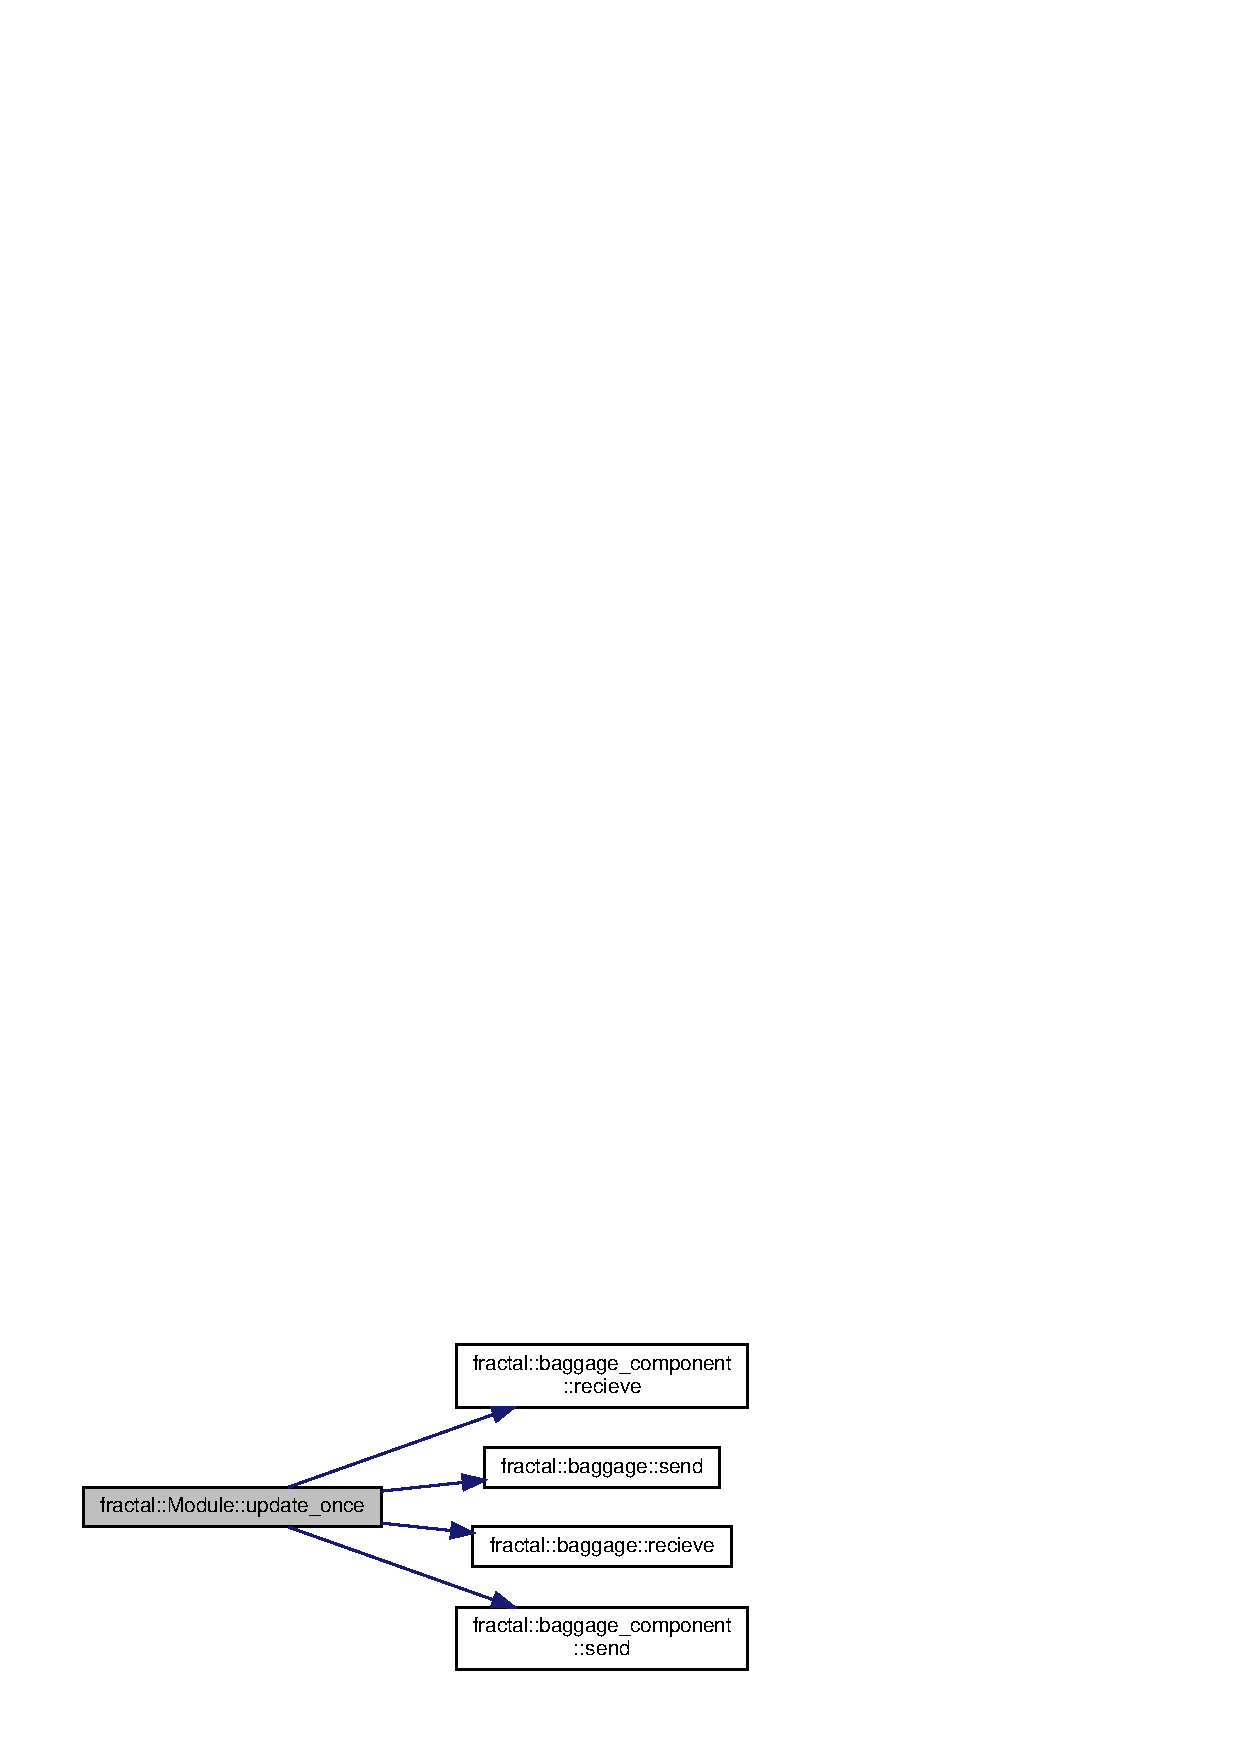
\includegraphics[width=350pt]{classfractal_1_1Module_abc2bf9795de848ecef0bd2e339a81e0d_cgraph}
\end{center}
\end{figure}


\subsection{メンバ詳解}
\mbox{\label{classfractal_1_1Module_a10311e3d5bff39ed0facbfe3b0eb9f0d}} 
\index{fractal\+::\+Module@{fractal\+::\+Module}!\+\_\+debug\+\_\+time\+\_\+view@{\+\_\+debug\+\_\+time\+\_\+view}}
\index{\+\_\+debug\+\_\+time\+\_\+view@{\+\_\+debug\+\_\+time\+\_\+view}!fractal\+::\+Module@{fractal\+::\+Module}}
\subsubsection{\texorpdfstring{\+\_\+debug\+\_\+time\+\_\+view}{\_debug\_time\_view}}
{\footnotesize\ttfamily bool fractal\+::\+Module\+::\+\_\+debug\+\_\+time\+\_\+view = false\hspace{0.3cm}{\ttfamily [private]}}

\mbox{\label{classfractal_1_1Module_adb17cd3c5a3edc29e0716d0f7abde9e8}} 
\index{fractal\+::\+Module@{fractal\+::\+Module}!\+\_\+debug\+\_\+time\+\_\+view\+\_\+dt@{\+\_\+debug\+\_\+time\+\_\+view\+\_\+dt}}
\index{\+\_\+debug\+\_\+time\+\_\+view\+\_\+dt@{\+\_\+debug\+\_\+time\+\_\+view\+\_\+dt}!fractal\+::\+Module@{fractal\+::\+Module}}
\subsubsection{\texorpdfstring{\+\_\+debug\+\_\+time\+\_\+view\+\_\+dt}{\_debug\_time\_view\_dt}}
{\footnotesize\ttfamily double fractal\+::\+Module\+::\+\_\+debug\+\_\+time\+\_\+view\+\_\+dt = 0.\+0\hspace{0.3cm}{\ttfamily [private]}}

\mbox{\label{classfractal_1_1Module_aed6038d7f13a217f171c3fa1a29e7129}} 
\index{fractal\+::\+Module@{fractal\+::\+Module}!\+\_\+is\+All\+Exit\+Message@{\+\_\+is\+All\+Exit\+Message}}
\index{\+\_\+is\+All\+Exit\+Message@{\+\_\+is\+All\+Exit\+Message}!fractal\+::\+Module@{fractal\+::\+Module}}
\subsubsection{\texorpdfstring{\+\_\+is\+All\+Exit\+Message}{\_isAllExitMessage}}
{\footnotesize\ttfamily bool fractal\+::\+Module\+::\+\_\+is\+All\+Exit\+Message = false\hspace{0.3cm}{\ttfamily [protected]}}



exit flag for all modules 

\mbox{\label{classfractal_1_1Module_ac1194f7c1723026348f7dc2df099ccf6}} 
\index{fractal\+::\+Module@{fractal\+::\+Module}!\+\_\+is\+Enable@{\+\_\+is\+Enable}}
\index{\+\_\+is\+Enable@{\+\_\+is\+Enable}!fractal\+::\+Module@{fractal\+::\+Module}}
\subsubsection{\texorpdfstring{\+\_\+is\+Enable}{\_isEnable}}
{\footnotesize\ttfamily bool fractal\+::\+Module\+::\+\_\+is\+Enable = true\hspace{0.3cm}{\ttfamily [protected]}}



status of this module 

\mbox{\label{classfractal_1_1Module_a3c0219468a7d043c70420cca57f39989}} 
\index{fractal\+::\+Module@{fractal\+::\+Module}!\+\_\+is\+Exit\+Message@{\+\_\+is\+Exit\+Message}}
\index{\+\_\+is\+Exit\+Message@{\+\_\+is\+Exit\+Message}!fractal\+::\+Module@{fractal\+::\+Module}}
\subsubsection{\texorpdfstring{\+\_\+is\+Exit\+Message}{\_isExitMessage}}
{\footnotesize\ttfamily bool fractal\+::\+Module\+::\+\_\+is\+Exit\+Message = false\hspace{0.3cm}{\ttfamily [protected]}}



exit flag for this modules 

\mbox{\label{classfractal_1_1Module_a36d598812541ddb73bb733dbcd708974}} 
\index{fractal\+::\+Module@{fractal\+::\+Module}!\+\_\+t@{\+\_\+t}}
\index{\+\_\+t@{\+\_\+t}!fractal\+::\+Module@{fractal\+::\+Module}}
\subsubsection{\texorpdfstring{\+\_\+t}{\_t}}
{\footnotesize\ttfamily \hyperlink{classfractal_1_1baggage}{baggage}$<$double$>$ fractal\+::\+Module\+::\+\_\+t = 0\hspace{0.3cm}{\ttfamily [private]}}



internal time 

\mbox{\label{classfractal_1_1Module_a8e59ac0be2426bde4e79a589ffc4cce4}} 
\index{fractal\+::\+Module@{fractal\+::\+Module}!message@{message}}
\index{message@{message}!fractal\+::\+Module@{fractal\+::\+Module}}
\subsubsection{\texorpdfstring{message}{message}}
{\footnotesize\ttfamily \hyperlink{classfractal_1_1baggage}{baggage}$<$std\+::string$>$ fractal\+::\+Module\+::message}



message 

\mbox{\label{classfractal_1_1Module_a47a4704bcfc9255a2e2ee8c81676a9f8}} 
\index{fractal\+::\+Module@{fractal\+::\+Module}!prev\+\_\+t@{prev\+\_\+t}}
\index{prev\+\_\+t@{prev\+\_\+t}!fractal\+::\+Module@{fractal\+::\+Module}}
\subsubsection{\texorpdfstring{prev\+\_\+t}{prev\_t}}
{\footnotesize\ttfamily double fractal\+::\+Module\+::prev\+\_\+t = 0\hspace{0.3cm}{\ttfamily [private]}}

\mbox{\label{classfractal_1_1Module_a8f01c07a782ebc8bbdab28212e275979}} 
\index{fractal\+::\+Module@{fractal\+::\+Module}!sleep\+\_\+time@{sleep\+\_\+time}}
\index{sleep\+\_\+time@{sleep\+\_\+time}!fractal\+::\+Module@{fractal\+::\+Module}}
\subsubsection{\texorpdfstring{sleep\+\_\+time}{sleep\_time}}
{\footnotesize\ttfamily double fractal\+::\+Module\+::sleep\+\_\+time = 0.\+0005\hspace{0.3cm}{\ttfamily [private]}}

\mbox{\label{classfractal_1_1Module_a869fe7b6421f11439ac696867a71d9eb}} 
\index{fractal\+::\+Module@{fractal\+::\+Module}!start@{start}}
\index{start@{start}!fractal\+::\+Module@{fractal\+::\+Module}}
\subsubsection{\texorpdfstring{start}{start}}
{\footnotesize\ttfamily std\+::chrono\+::system\+\_\+clock\+::time\+\_\+point fractal\+::\+Module\+::start\hspace{0.3cm}{\ttfamily [private]}}

\mbox{\label{classfractal_1_1Module_ac14a8d440a0a4f7a0be952a902c3717e}} 
\index{fractal\+::\+Module@{fractal\+::\+Module}!t@{t}}
\index{t@{t}!fractal\+::\+Module@{fractal\+::\+Module}}
\subsubsection{\texorpdfstring{t}{t}}
{\footnotesize\ttfamily \hyperlink{classfractal_1_1baggage}{baggage}$<$double$>$ fractal\+::\+Module\+::t = 0}



synchronization time 



このクラス詳解は次のファイルから抽出されました\+:\begin{DoxyCompactItemize}
\item 
/home/takanobu/fractal/include/\hyperlink{fractal_8h}{fractal.\+h}\end{DoxyCompactItemize}

\section{fractal\+:\+:baggage$<$ T $>$\+:\+:safe\+\_\+data 構造体}
\label{structfractal_1_1baggage_1_1safe__data}\index{fractal\+::baggage$<$ T $>$\+::safe\+\_\+data@{fractal\+::baggage$<$ T $>$\+::safe\+\_\+data}}


safe data structure  




fractal\+:\+:baggage$<$ T $>$\+:\+:safe\+\_\+data 連携図
\nopagebreak
\begin{figure}[H]
\begin{center}
\leavevmode
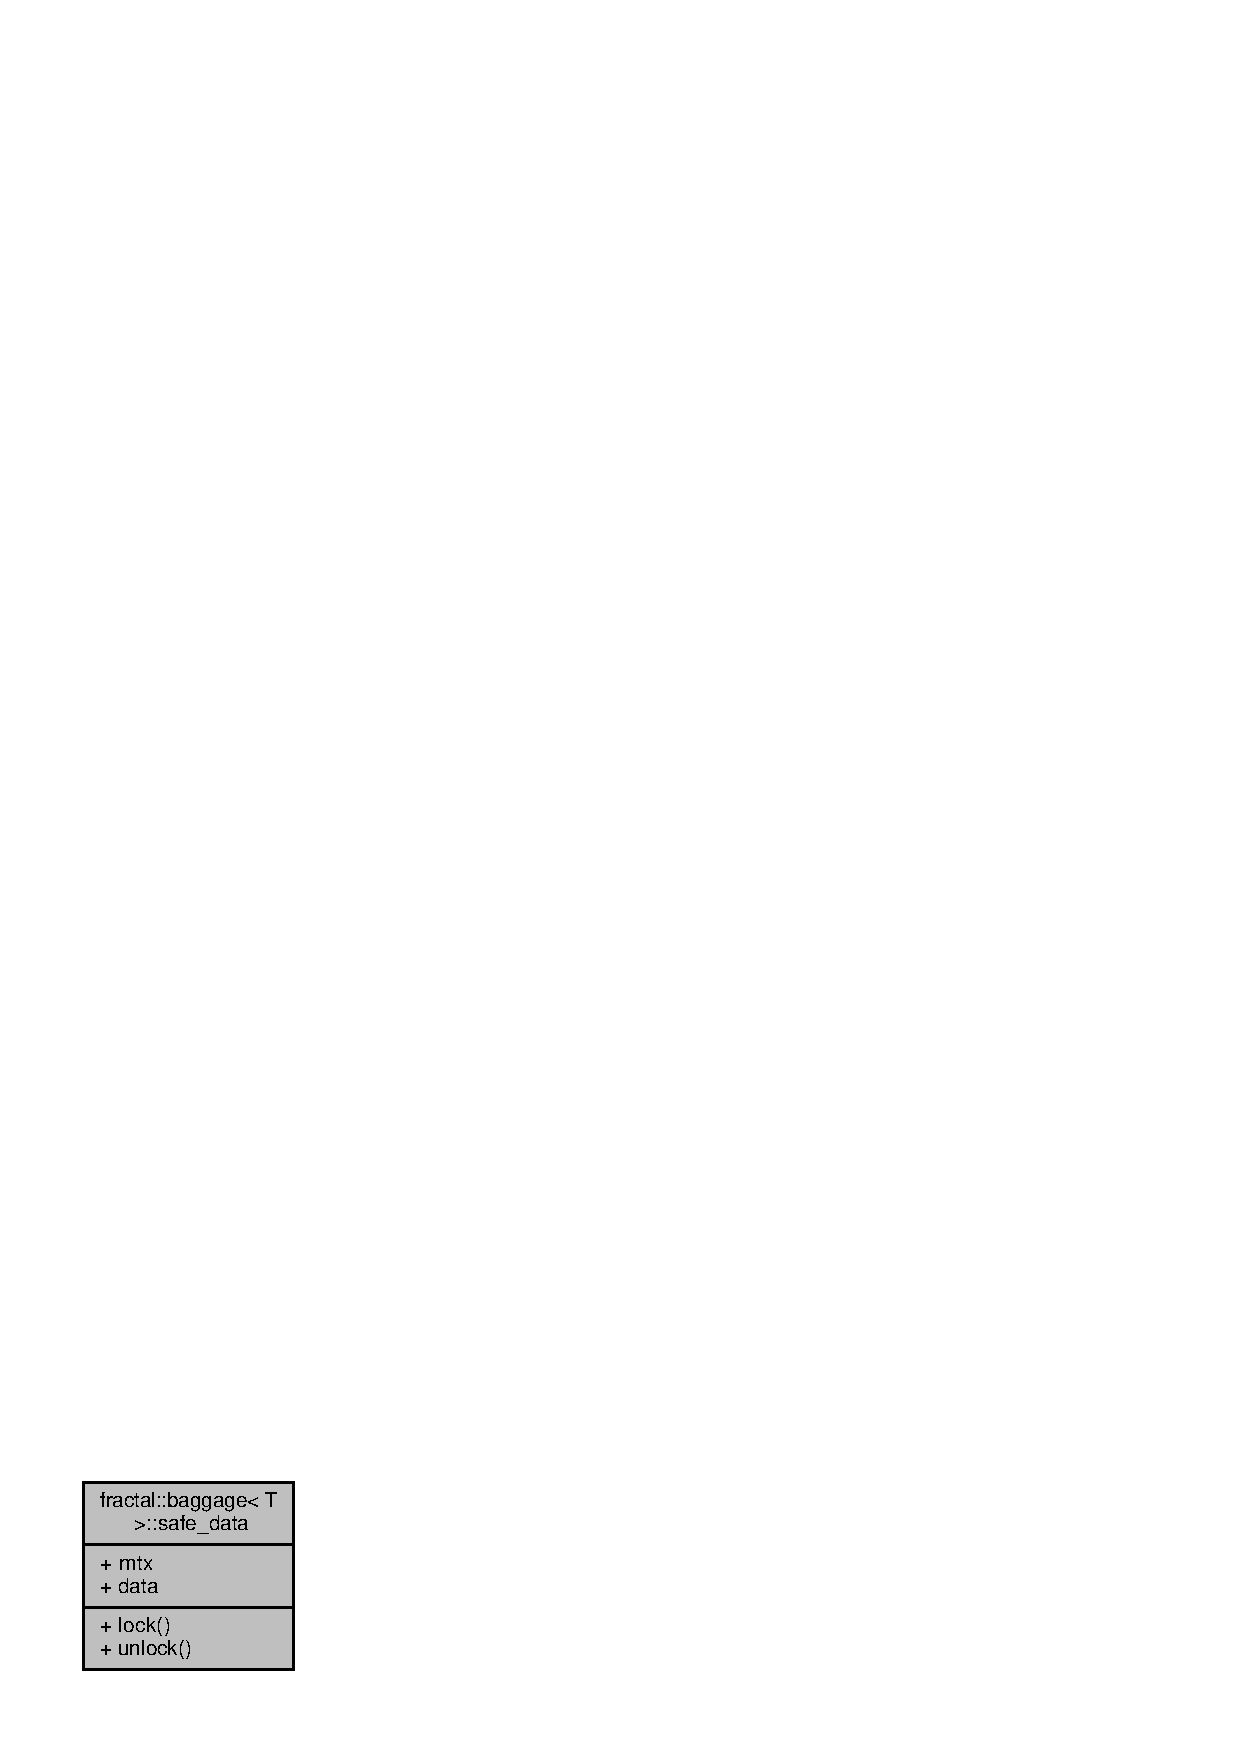
\includegraphics[width=145pt]{structfractal_1_1baggage_1_1safe__data__coll__graph}
\end{center}
\end{figure}
\subsection*{公開メンバ関数}
\begin{DoxyCompactItemize}
\item 
void \hyperlink{structfractal_1_1baggage_1_1safe__data_aa441d027dbf60530c88a586a758e862e}{lock} ()
\item 
void \hyperlink{structfractal_1_1baggage_1_1safe__data_a7e1acde240d0f75ad744edfc114cdf55}{unlock} ()
\end{DoxyCompactItemize}
\subsection*{公開変数類}
\begin{DoxyCompactItemize}
\item 
std\+::mutex \hyperlink{structfractal_1_1baggage_1_1safe__data_a7a9929c47da7c72ea70f4f0b47609bc8}{mtx}
\begin{DoxyCompactList}\small\item\em mutex class \end{DoxyCompactList}\item 
T \hyperlink{structfractal_1_1baggage_1_1safe__data_afd9e1db72a670350da2a7fe2dbb17376}{data}
\begin{DoxyCompactList}\small\item\em data \end{DoxyCompactList}\end{DoxyCompactItemize}


\subsection{詳解}
\subsubsection*{template$<$class T$>$\newline
struct fractal\+::baggage$<$ T $>$\+::safe\+\_\+data}

safe data structure 

mutex and data 

\subsection{関数詳解}
\mbox{\label{structfractal_1_1baggage_1_1safe__data_aa441d027dbf60530c88a586a758e862e}} 
\index{fractal\+::baggage\+::safe\+\_\+data@{fractal\+::baggage\+::safe\+\_\+data}!lock@{lock}}
\index{lock@{lock}!fractal\+::baggage\+::safe\+\_\+data@{fractal\+::baggage\+::safe\+\_\+data}}
\subsubsection{\texorpdfstring{lock()}{lock()}}
{\footnotesize\ttfamily template$<$class T$>$ \\
void \hyperlink{classfractal_1_1baggage}{fractal\+::baggage}$<$ T $>$\+::safe\+\_\+data\+::lock (\begin{DoxyParamCaption}{ }\end{DoxyParamCaption})\hspace{0.3cm}{\ttfamily [inline]}}

\mbox{\label{structfractal_1_1baggage_1_1safe__data_a7e1acde240d0f75ad744edfc114cdf55}} 
\index{fractal\+::baggage\+::safe\+\_\+data@{fractal\+::baggage\+::safe\+\_\+data}!unlock@{unlock}}
\index{unlock@{unlock}!fractal\+::baggage\+::safe\+\_\+data@{fractal\+::baggage\+::safe\+\_\+data}}
\subsubsection{\texorpdfstring{unlock()}{unlock()}}
{\footnotesize\ttfamily template$<$class T$>$ \\
void \hyperlink{classfractal_1_1baggage}{fractal\+::baggage}$<$ T $>$\+::safe\+\_\+data\+::unlock (\begin{DoxyParamCaption}{ }\end{DoxyParamCaption})\hspace{0.3cm}{\ttfamily [inline]}}



\subsection{メンバ詳解}
\mbox{\label{structfractal_1_1baggage_1_1safe__data_afd9e1db72a670350da2a7fe2dbb17376}} 
\index{fractal\+::baggage\+::safe\+\_\+data@{fractal\+::baggage\+::safe\+\_\+data}!data@{data}}
\index{data@{data}!fractal\+::baggage\+::safe\+\_\+data@{fractal\+::baggage\+::safe\+\_\+data}}
\subsubsection{\texorpdfstring{data}{data}}
{\footnotesize\ttfamily template$<$class T$>$ \\
T \hyperlink{classfractal_1_1baggage}{fractal\+::baggage}$<$ T $>$\+::safe\+\_\+data\+::data}



data 

\mbox{\label{structfractal_1_1baggage_1_1safe__data_a7a9929c47da7c72ea70f4f0b47609bc8}} 
\index{fractal\+::baggage\+::safe\+\_\+data@{fractal\+::baggage\+::safe\+\_\+data}!mtx@{mtx}}
\index{mtx@{mtx}!fractal\+::baggage\+::safe\+\_\+data@{fractal\+::baggage\+::safe\+\_\+data}}
\subsubsection{\texorpdfstring{mtx}{mtx}}
{\footnotesize\ttfamily template$<$class T$>$ \\
std\+::mutex \hyperlink{classfractal_1_1baggage}{fractal\+::baggage}$<$ T $>$\+::safe\+\_\+data\+::mtx}



mutex class 



この構造体詳解は次のファイルから抽出されました\+:\begin{DoxyCompactItemize}
\item 
/home/takanobu/fractal/include/\hyperlink{fractal_8h}{fractal.\+h}\end{DoxyCompactItemize}

\section{fractal\+:\+:System クラス}
\label{classfractal_1_1System}\index{fractal\+::\+System@{fractal\+::\+System}}


\hyperlink{classfractal_1_1System}{System} Class  




{\ttfamily \#include $<$fractal.\+h$>$}



fractal\+:\+:System の継承関係図
\nopagebreak
\begin{figure}[H]
\begin{center}
\leavevmode
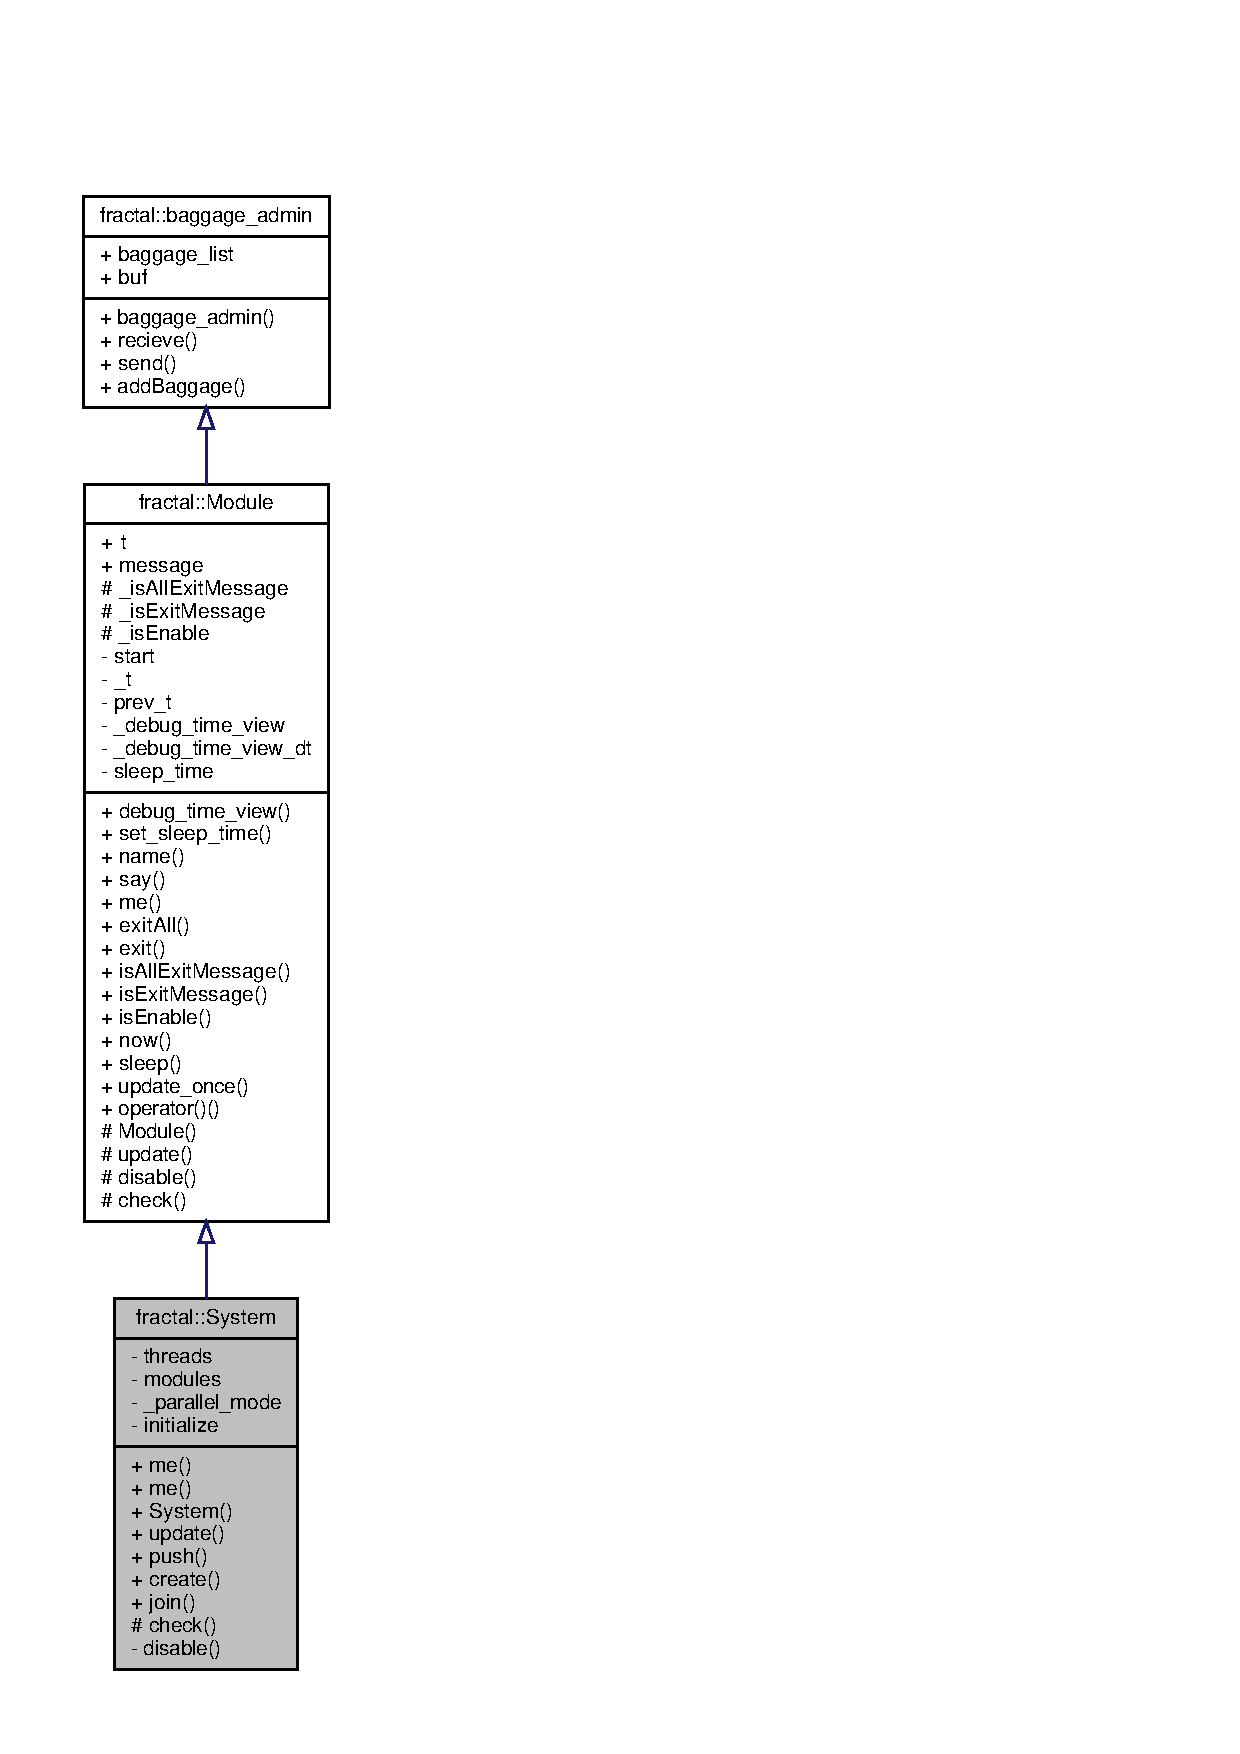
\includegraphics[height=550pt]{classfractal_1_1System__inherit__graph}
\end{center}
\end{figure}


fractal\+:\+:System 連携図
\nopagebreak
\begin{figure}[H]
\begin{center}
\leavevmode
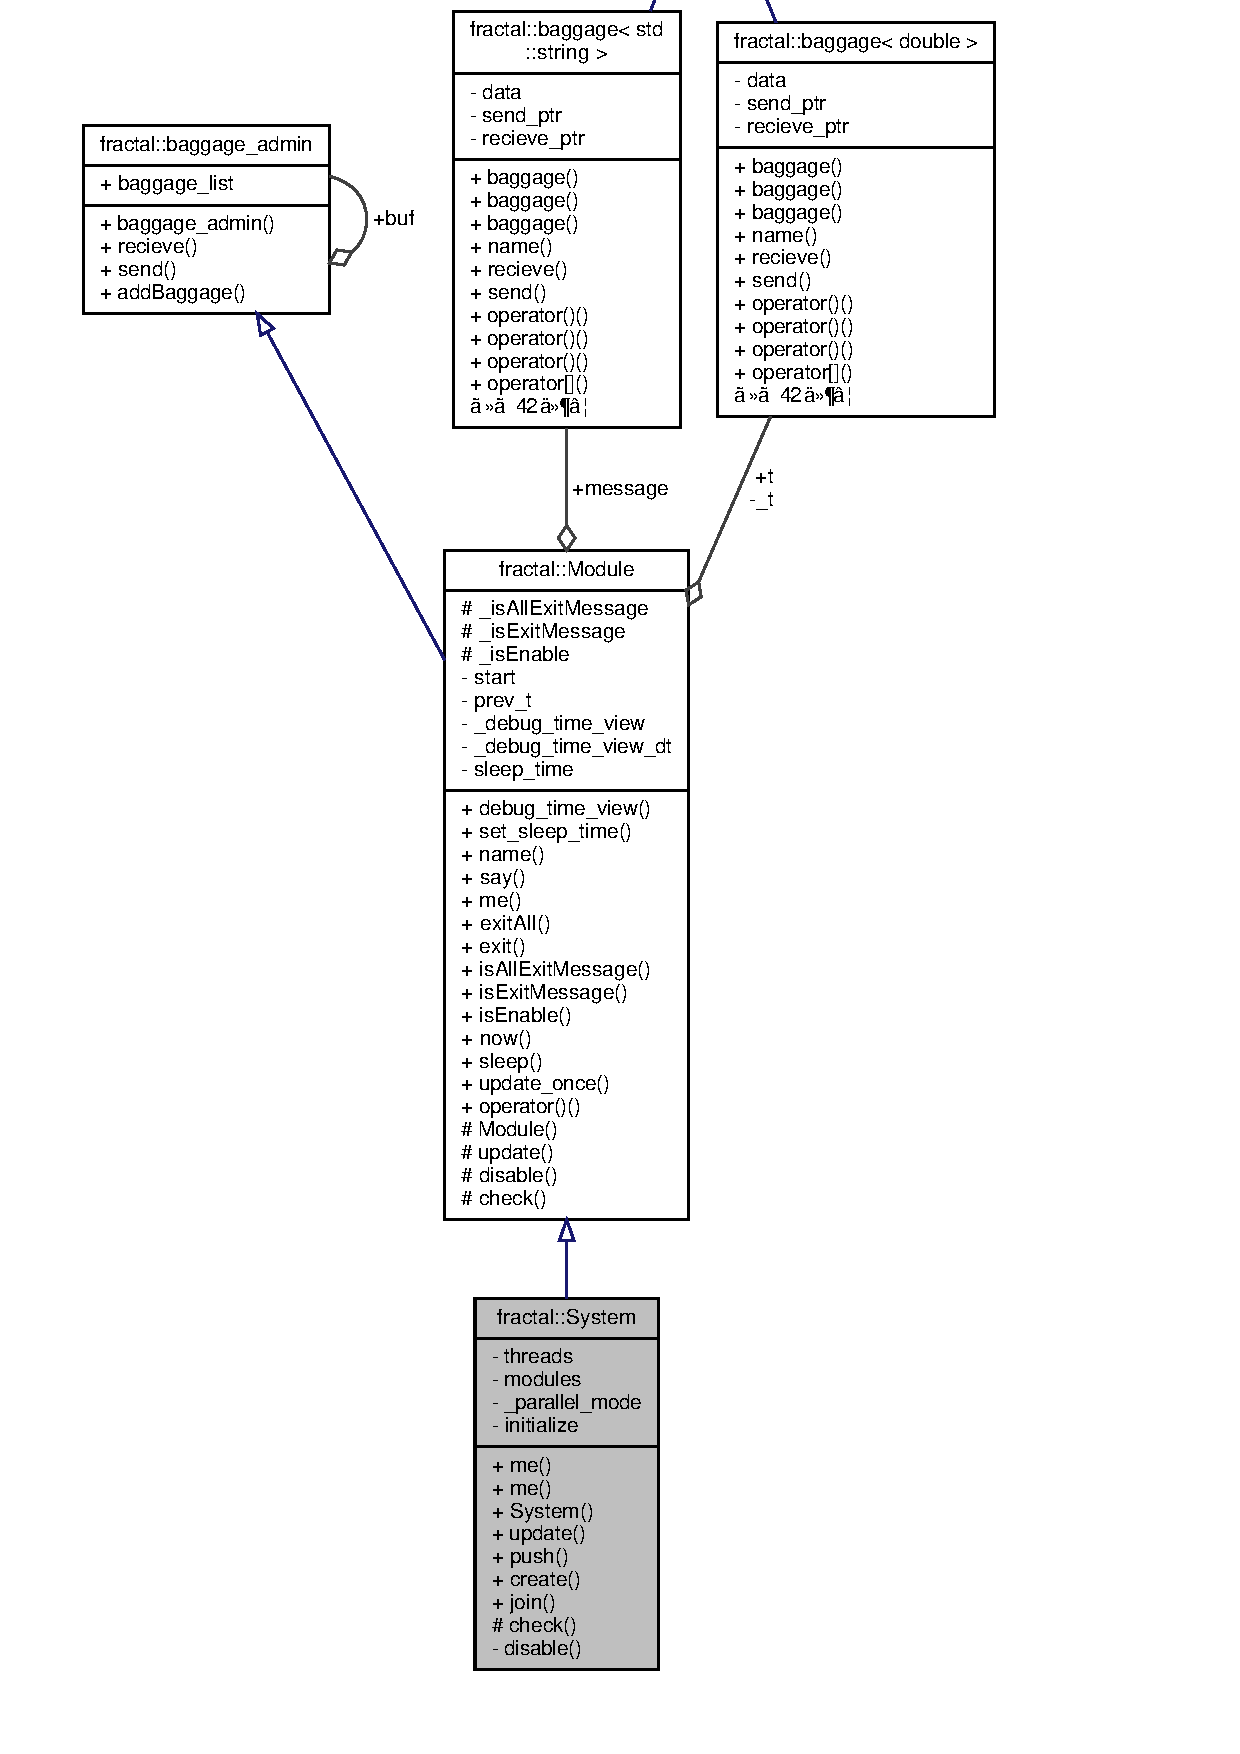
\includegraphics[height=550pt]{classfractal_1_1System__coll__graph}
\end{center}
\end{figure}
\subsection*{公開メンバ関数}
\begin{DoxyCompactItemize}
\item 
virtual void \hyperlink{classfractal_1_1System_aa8e8768417ccfe745def786d63eee80d}{me} (int n)
\begin{DoxyCompactList}\small\item\em show system layer \end{DoxyCompactList}\item 
void \hyperlink{classfractal_1_1System_ae1da12b267d3fe5b811e4130ae888b50}{me} ()
\begin{DoxyCompactList}\small\item\em show system structure \end{DoxyCompactList}\item 
\hyperlink{classfractal_1_1System_a2d135113ff09a5cce9871ab696b40087}{System} (bool parallel\+\_\+mode=false)
\item 
virtual void \hyperlink{classfractal_1_1System_a86fe5dae233bd52be06fe950087787d9}{update} (double dt)
\begin{DoxyCompactList}\small\item\em update function \end{DoxyCompactList}\item 
void \hyperlink{classfractal_1_1System_a69dd1513fed01dd3cf455763bd243f5e}{push} (\hyperlink{classfractal_1_1Module}{Module} $\ast$ptr)
\item 
void \hyperlink{classfractal_1_1System_a00d5baae4bcc777c43da65299b464a43}{create} ()
\item 
void \hyperlink{classfractal_1_1System_afcd530ae6b4fd18a74fb807e56bd5fff}{join} ()
\end{DoxyCompactItemize}
\subsection*{限定公開メンバ関数}
\begin{DoxyCompactItemize}
\item 
virtual void \hyperlink{classfractal_1_1System_a95f99e9132a10f87f9179a27c840fa50}{check} ()
\begin{DoxyCompactList}\small\item\em  check exit message \end{DoxyCompactList}\end{DoxyCompactItemize}
\subsection*{非公開メンバ関数}
\begin{DoxyCompactItemize}
\item 
virtual void \hyperlink{classfractal_1_1System_a446532d4c3811f6005e0c52ad653a997}{disable} ()
\begin{DoxyCompactList}\small\item\em disable this system \end{DoxyCompactList}\end{DoxyCompactItemize}
\subsection*{非公開変数類}
\begin{DoxyCompactItemize}
\item 
std\+::vector$<$ std\+::thread $>$ \hyperlink{classfractal_1_1System_a6da1d544119f50d90f71cf7d4ba53007}{threads}
\begin{DoxyCompactList}\small\item\em thread list \end{DoxyCompactList}\item 
std\+::vector$<$ \hyperlink{classfractal_1_1Module}{Module} $\ast$ $>$ \hyperlink{classfractal_1_1System_ab458c473c6203ab1f82adb08cdada89a}{modules}
\begin{DoxyCompactList}\small\item\em module list \end{DoxyCompactList}\item 
bool \hyperlink{classfractal_1_1System_a740b45f120349f503425770aa3926863}{\+\_\+parallel\+\_\+mode}
\item 
bool \hyperlink{classfractal_1_1System_aa14a55323502d83d3e2f949dd33e0747}{initialize} = true
\end{DoxyCompactItemize}
\subsection*{その他の継承メンバ}


\subsection{詳解}
\hyperlink{classfractal_1_1System}{System} Class 

base class for system 

\subsection{構築子と解体子}
\mbox{\label{classfractal_1_1System_a2d135113ff09a5cce9871ab696b40087}} 
\index{fractal\+::\+System@{fractal\+::\+System}!System@{System}}
\index{System@{System}!fractal\+::\+System@{fractal\+::\+System}}
\subsubsection{\texorpdfstring{System()}{System()}}
{\footnotesize\ttfamily fractal\+::\+System\+::\+System (\begin{DoxyParamCaption}\item[{bool}]{parallel\+\_\+mode = {\ttfamily false} }\end{DoxyParamCaption})\hspace{0.3cm}{\ttfamily [inline]}}



\subsection{関数詳解}
\mbox{\label{classfractal_1_1System_a95f99e9132a10f87f9179a27c840fa50}} 
\index{fractal\+::\+System@{fractal\+::\+System}!check@{check}}
\index{check@{check}!fractal\+::\+System@{fractal\+::\+System}}
\subsubsection{\texorpdfstring{check()}{check()}}
{\footnotesize\ttfamily virtual void fractal\+::\+System\+::check (\begin{DoxyParamCaption}\item[{void}]{ }\end{DoxyParamCaption})\hspace{0.3cm}{\ttfamily [inline]}, {\ttfamily [protected]}, {\ttfamily [virtual]}}



 check exit message 



\hyperlink{classfractal_1_1Module_a245865f346ac1d21b19bce418bf704c4}{fractal\+::\+Module}を再実装しています。

\mbox{\label{classfractal_1_1System_a00d5baae4bcc777c43da65299b464a43}} 
\index{fractal\+::\+System@{fractal\+::\+System}!create@{create}}
\index{create@{create}!fractal\+::\+System@{fractal\+::\+System}}
\subsubsection{\texorpdfstring{create()}{create()}}
{\footnotesize\ttfamily void fractal\+::\+System\+::create (\begin{DoxyParamCaption}{ }\end{DoxyParamCaption})\hspace{0.3cm}{\ttfamily [inline]}}

\mbox{\label{classfractal_1_1System_a446532d4c3811f6005e0c52ad653a997}} 
\index{fractal\+::\+System@{fractal\+::\+System}!disable@{disable}}
\index{disable@{disable}!fractal\+::\+System@{fractal\+::\+System}}
\subsubsection{\texorpdfstring{disable()}{disable()}}
{\footnotesize\ttfamily virtual void fractal\+::\+System\+::disable (\begin{DoxyParamCaption}\item[{void}]{ }\end{DoxyParamCaption})\hspace{0.3cm}{\ttfamily [inline]}, {\ttfamily [private]}, {\ttfamily [virtual]}}



disable this system 



\hyperlink{classfractal_1_1Module_a17a7773769fb523fd4b2aeb28366debe}{fractal\+::\+Module}を再実装しています。

\mbox{\label{classfractal_1_1System_afcd530ae6b4fd18a74fb807e56bd5fff}} 
\index{fractal\+::\+System@{fractal\+::\+System}!join@{join}}
\index{join@{join}!fractal\+::\+System@{fractal\+::\+System}}
\subsubsection{\texorpdfstring{join()}{join()}}
{\footnotesize\ttfamily void fractal\+::\+System\+::join (\begin{DoxyParamCaption}{ }\end{DoxyParamCaption})\hspace{0.3cm}{\ttfamily [inline]}}

\mbox{\label{classfractal_1_1System_aa8e8768417ccfe745def786d63eee80d}} 
\index{fractal\+::\+System@{fractal\+::\+System}!me@{me}}
\index{me@{me}!fractal\+::\+System@{fractal\+::\+System}}
\subsubsection{\texorpdfstring{me()}{me()}\hspace{0.1cm}{\footnotesize\ttfamily [1/2]}}
{\footnotesize\ttfamily virtual void fractal\+::\+System\+::me (\begin{DoxyParamCaption}\item[{int}]{n }\end{DoxyParamCaption})\hspace{0.3cm}{\ttfamily [inline]}, {\ttfamily [virtual]}}



show system layer 


\begin{DoxyParams}{引数}
{\em n} & layer number \\
\hline
\end{DoxyParams}


\hyperlink{classfractal_1_1Module_a92deaafb88a2bc34958dca99fdc112a3}{fractal\+::\+Module}を再実装しています。

\mbox{\label{classfractal_1_1System_ae1da12b267d3fe5b811e4130ae888b50}} 
\index{fractal\+::\+System@{fractal\+::\+System}!me@{me}}
\index{me@{me}!fractal\+::\+System@{fractal\+::\+System}}
\subsubsection{\texorpdfstring{me()}{me()}\hspace{0.1cm}{\footnotesize\ttfamily [2/2]}}
{\footnotesize\ttfamily void fractal\+::\+System\+::me (\begin{DoxyParamCaption}{ }\end{DoxyParamCaption})\hspace{0.3cm}{\ttfamily [inline]}}



show system structure 

呼び出し関係図\+:
\nopagebreak
\begin{figure}[H]
\begin{center}
\leavevmode
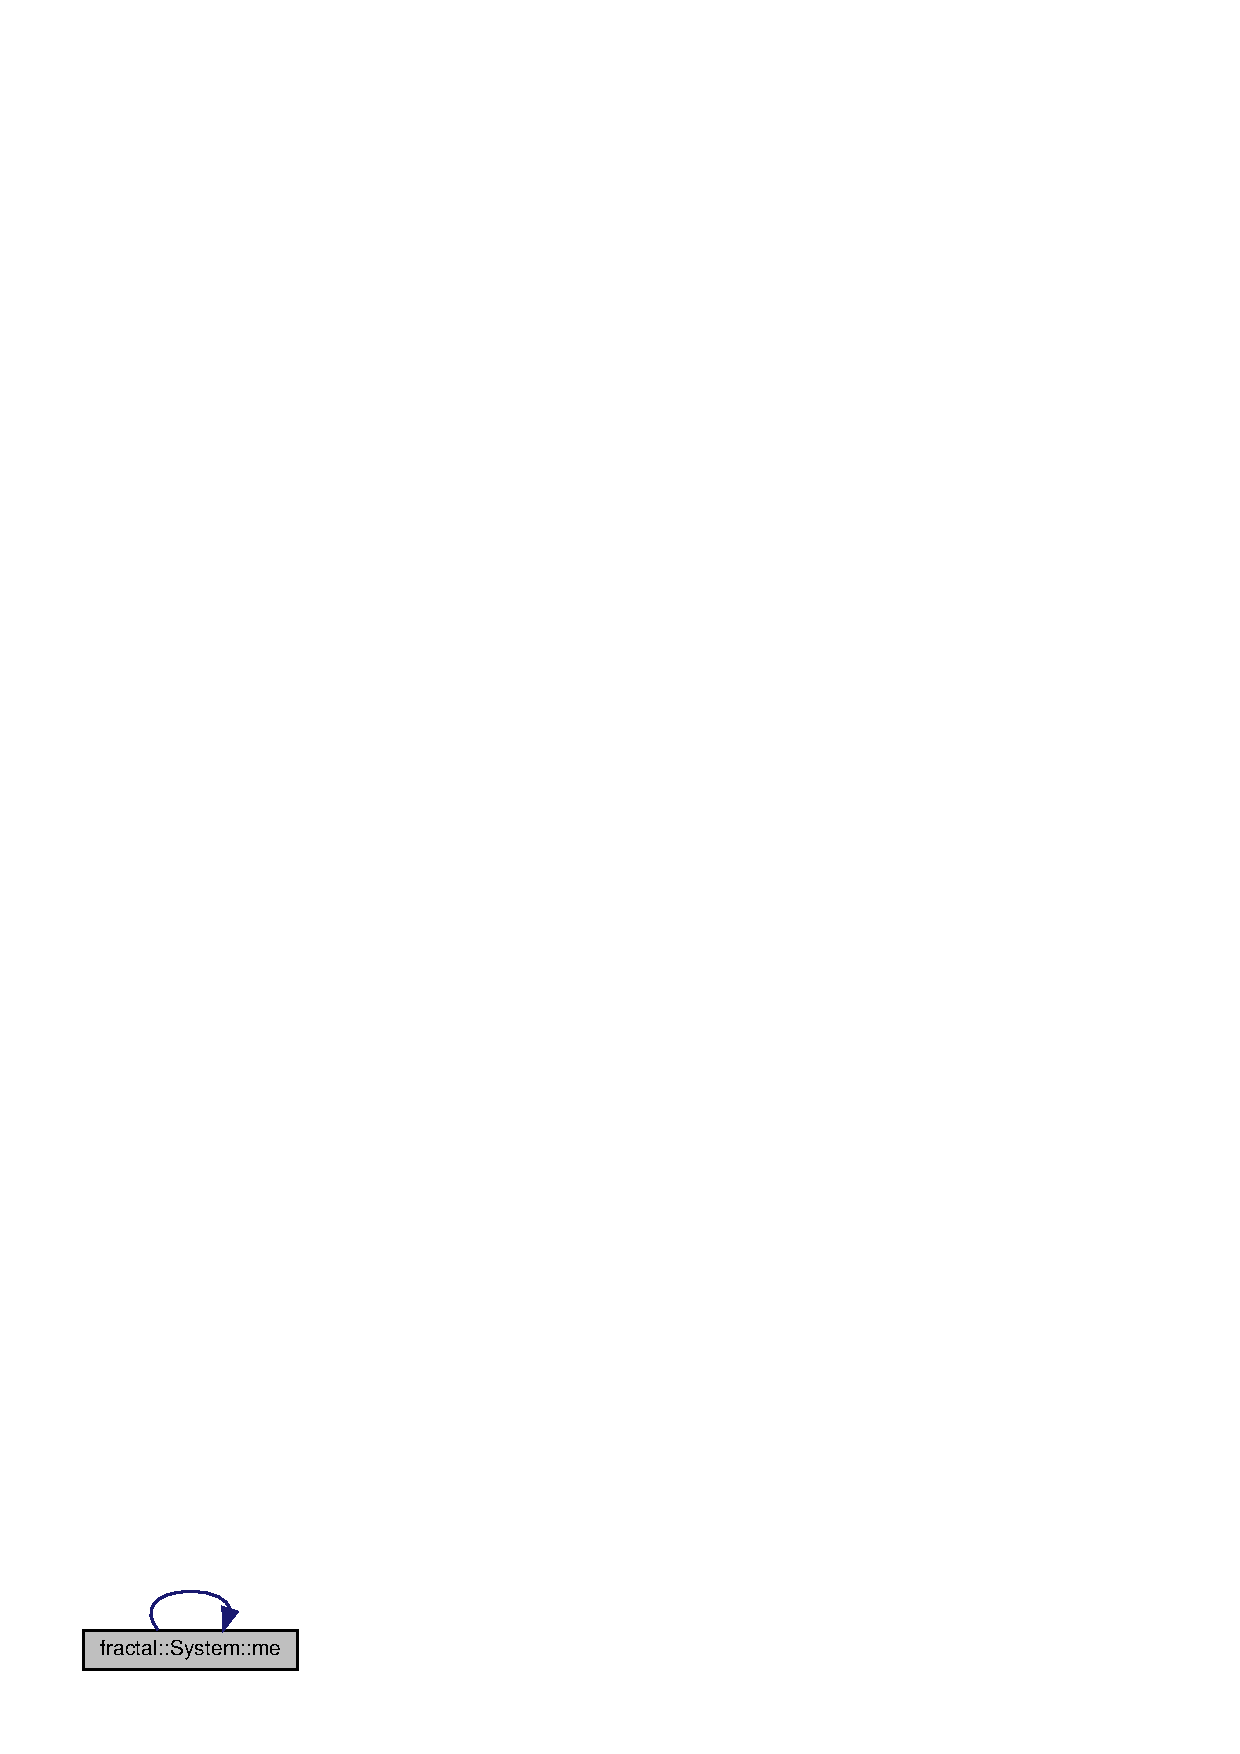
\includegraphics[width=147pt]{classfractal_1_1System_ae1da12b267d3fe5b811e4130ae888b50_cgraph}
\end{center}
\end{figure}
被呼び出し関係図\+:
\nopagebreak
\begin{figure}[H]
\begin{center}
\leavevmode
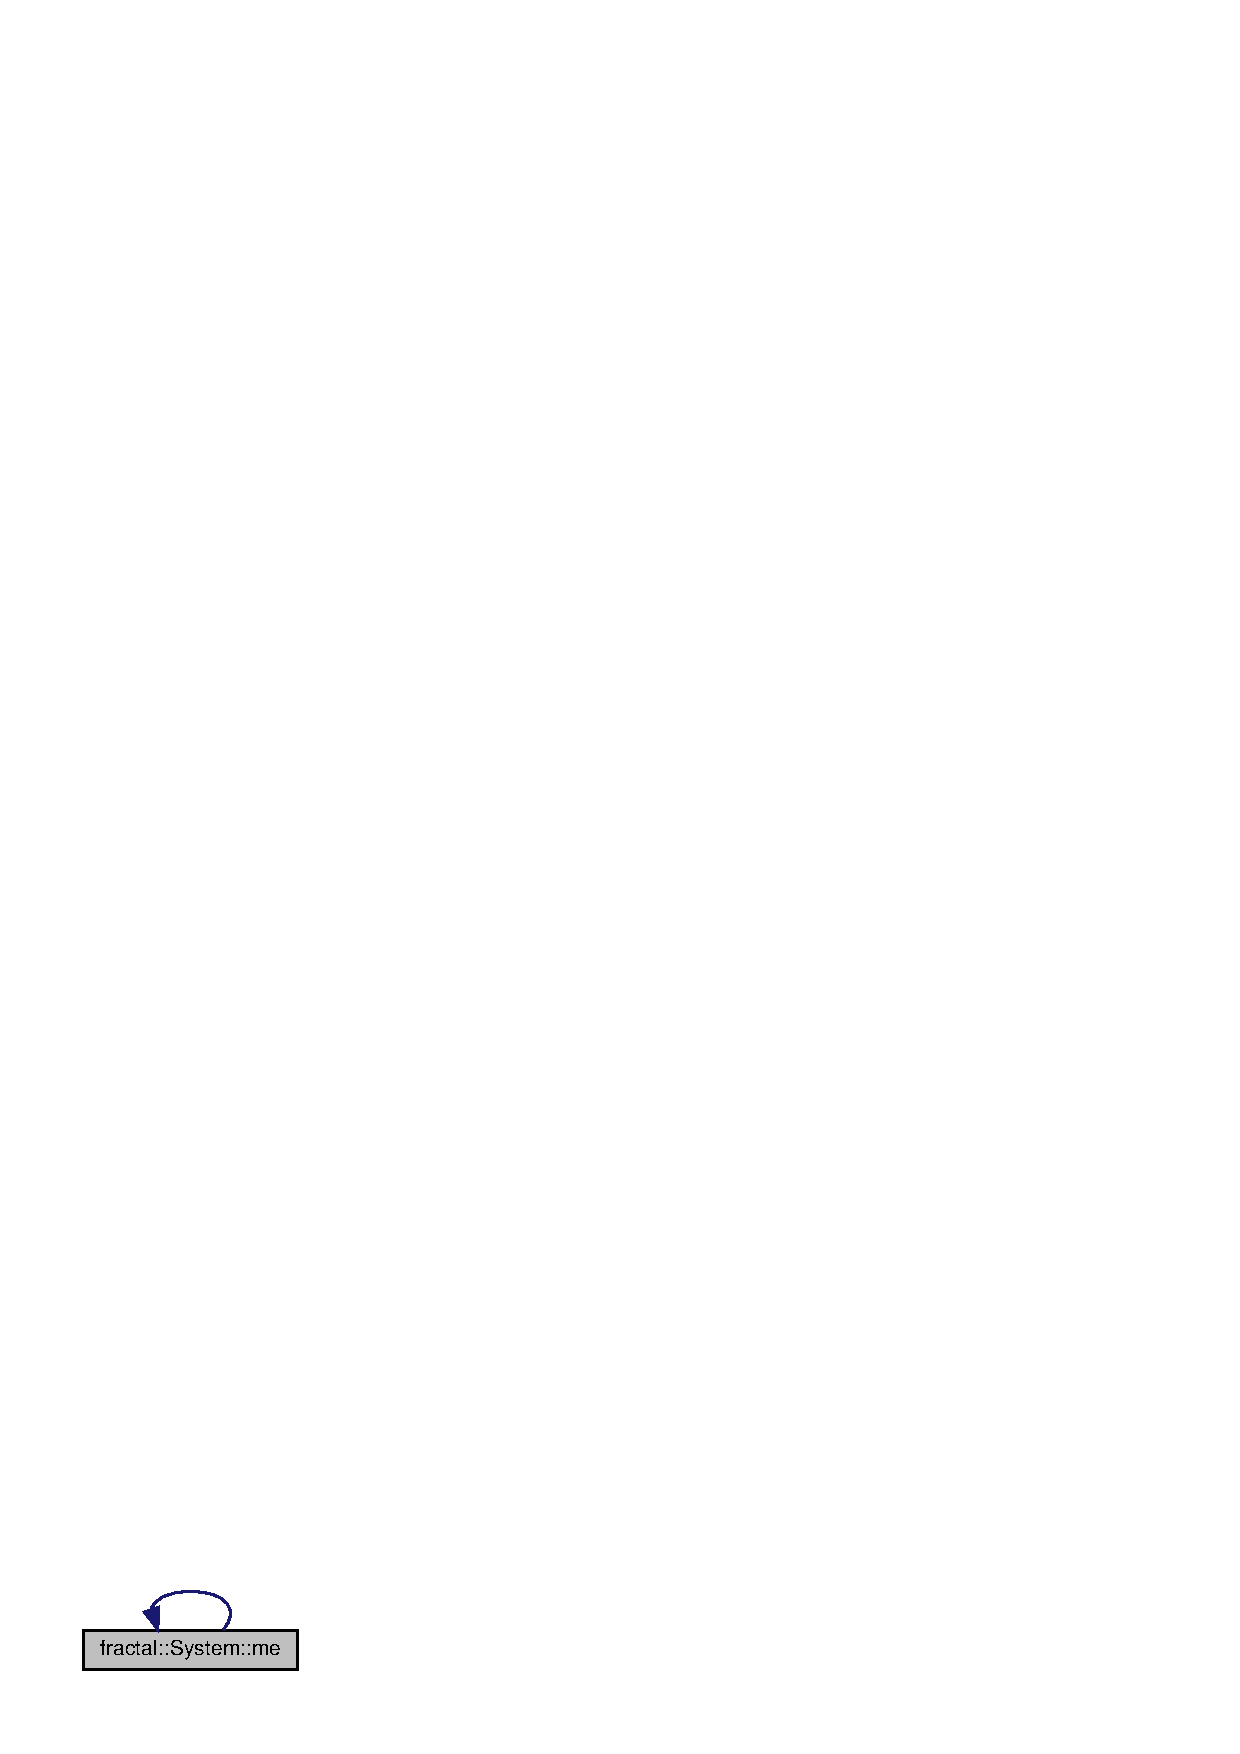
\includegraphics[width=147pt]{classfractal_1_1System_ae1da12b267d3fe5b811e4130ae888b50_icgraph}
\end{center}
\end{figure}
\mbox{\label{classfractal_1_1System_a69dd1513fed01dd3cf455763bd243f5e}} 
\index{fractal\+::\+System@{fractal\+::\+System}!push@{push}}
\index{push@{push}!fractal\+::\+System@{fractal\+::\+System}}
\subsubsection{\texorpdfstring{push()}{push()}}
{\footnotesize\ttfamily void fractal\+::\+System\+::push (\begin{DoxyParamCaption}\item[{\hyperlink{classfractal_1_1Module}{Module} $\ast$}]{ptr }\end{DoxyParamCaption})\hspace{0.3cm}{\ttfamily [inline]}}

呼び出し関係図\+:
\nopagebreak
\begin{figure}[H]
\begin{center}
\leavevmode
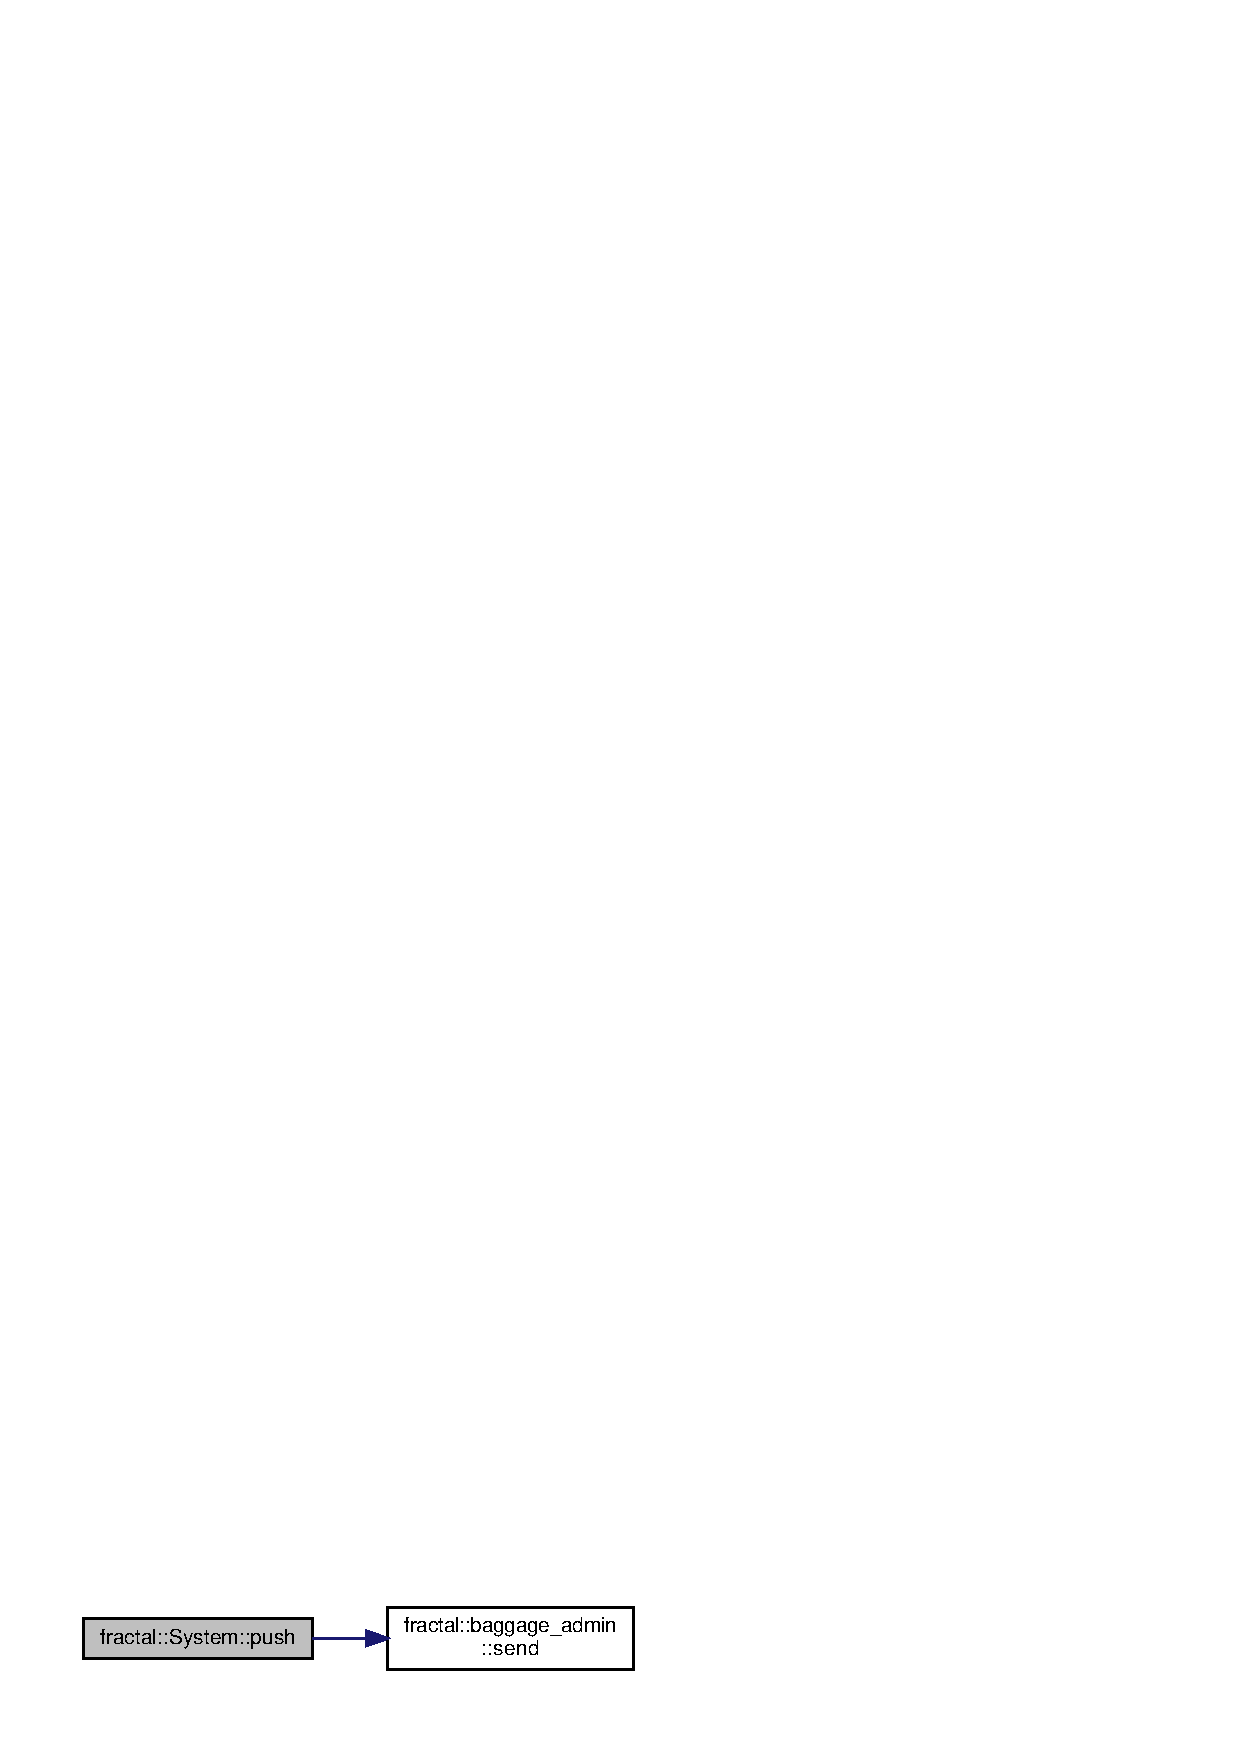
\includegraphics[width=308pt]{classfractal_1_1System_a69dd1513fed01dd3cf455763bd243f5e_cgraph}
\end{center}
\end{figure}
\mbox{\label{classfractal_1_1System_a86fe5dae233bd52be06fe950087787d9}} 
\index{fractal\+::\+System@{fractal\+::\+System}!update@{update}}
\index{update@{update}!fractal\+::\+System@{fractal\+::\+System}}
\subsubsection{\texorpdfstring{update()}{update()}}
{\footnotesize\ttfamily virtual void fractal\+::\+System\+::update (\begin{DoxyParamCaption}\item[{double}]{dt }\end{DoxyParamCaption})\hspace{0.3cm}{\ttfamily [inline]}, {\ttfamily [virtual]}}



update function 


\begin{DoxyParams}{引数}
{\em dt} & delta time\\
\hline
\end{DoxyParams}
redefine in derived classes 

\hyperlink{classfractal_1_1Module_ad68342ebc960bb0e1dd19b7c70bc3753}{fractal\+::\+Module}を再実装しています。



\subsection{メンバ詳解}
\mbox{\label{classfractal_1_1System_a740b45f120349f503425770aa3926863}} 
\index{fractal\+::\+System@{fractal\+::\+System}!\+\_\+parallel\+\_\+mode@{\+\_\+parallel\+\_\+mode}}
\index{\+\_\+parallel\+\_\+mode@{\+\_\+parallel\+\_\+mode}!fractal\+::\+System@{fractal\+::\+System}}
\subsubsection{\texorpdfstring{\+\_\+parallel\+\_\+mode}{\_parallel\_mode}}
{\footnotesize\ttfamily bool fractal\+::\+System\+::\+\_\+parallel\+\_\+mode\hspace{0.3cm}{\ttfamily [private]}}

\mbox{\label{classfractal_1_1System_aa14a55323502d83d3e2f949dd33e0747}} 
\index{fractal\+::\+System@{fractal\+::\+System}!initialize@{initialize}}
\index{initialize@{initialize}!fractal\+::\+System@{fractal\+::\+System}}
\subsubsection{\texorpdfstring{initialize}{initialize}}
{\footnotesize\ttfamily bool fractal\+::\+System\+::initialize = true\hspace{0.3cm}{\ttfamily [private]}}

\mbox{\label{classfractal_1_1System_ab458c473c6203ab1f82adb08cdada89a}} 
\index{fractal\+::\+System@{fractal\+::\+System}!modules@{modules}}
\index{modules@{modules}!fractal\+::\+System@{fractal\+::\+System}}
\subsubsection{\texorpdfstring{modules}{modules}}
{\footnotesize\ttfamily std\+::vector$<$\hyperlink{classfractal_1_1Module}{Module} $\ast$$>$ fractal\+::\+System\+::modules\hspace{0.3cm}{\ttfamily [private]}}



module list 

\mbox{\label{classfractal_1_1System_a6da1d544119f50d90f71cf7d4ba53007}} 
\index{fractal\+::\+System@{fractal\+::\+System}!threads@{threads}}
\index{threads@{threads}!fractal\+::\+System@{fractal\+::\+System}}
\subsubsection{\texorpdfstring{threads}{threads}}
{\footnotesize\ttfamily std\+::vector$<$std\+::thread$>$ fractal\+::\+System\+::threads\hspace{0.3cm}{\ttfamily [private]}}



thread list 



このクラス詳解は次のファイルから抽出されました\+:\begin{DoxyCompactItemize}
\item 
/home/takanobu/fractal/include/\hyperlink{fractal_8h}{fractal.\+h}\end{DoxyCompactItemize}

\chapter{ファイル詳解}
\section{/home/takanobu/fractal/include/fractal.h ファイル}
\label{fractal_8h}\index{/home/takanobu/fractal/include/fractal.\+h@{/home/takanobu/fractal/include/fractal.\+h}}


Parallel System Module  


{\ttfamily \#include $<$iostream$>$}\newline
{\ttfamily \#include $<$string$>$}\newline
{\ttfamily \#include $<$tuple$>$}\newline
{\ttfamily \#include $<$vector$>$}\newline
{\ttfamily \#include $<$mutex$>$}\newline
{\ttfamily \#include $<$thread$>$}\newline
{\ttfamily \#include $<$chrono$>$}\newline
{\ttfamily \#include $<$unistd.\+h$>$}\newline
{\ttfamily \#include $<$functional$>$}\newline
{\ttfamily \#include $<$typeinfo$>$}\newline
{\ttfamily \#include $<$cxxabi.\+h$>$}\newline
{\ttfamily \#include $<$sstream$>$}\newline
fractal.\+h の依存先関係図\+:
\nopagebreak
\begin{figure}[H]
\begin{center}
\leavevmode
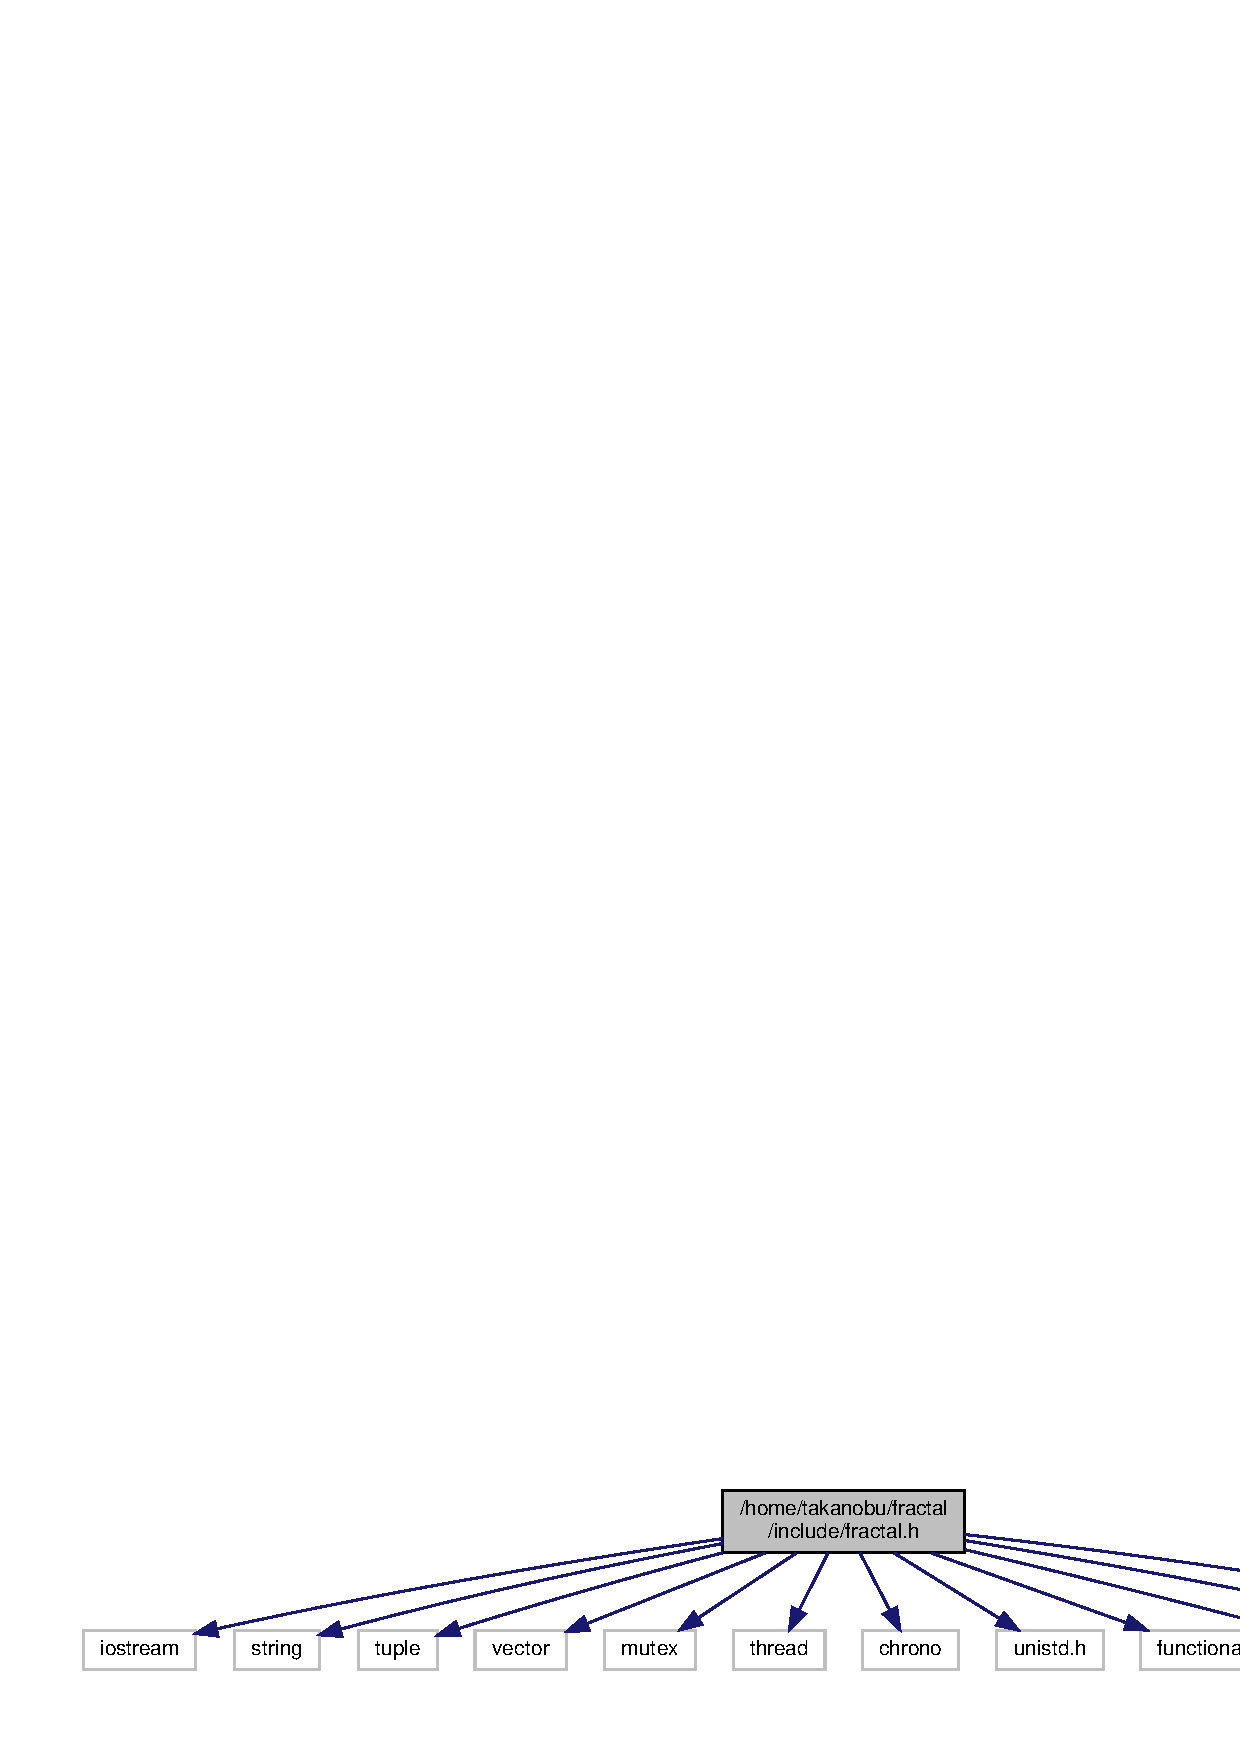
\includegraphics[width=350pt]{fractal_8h__incl}
\end{center}
\end{figure}
\subsection*{クラス}
\begin{DoxyCompactItemize}
\item 
class \hyperlink{classfractal_1_1baggage__component}{fractal\+::baggage\+\_\+component}
\item 
class \hyperlink{classfractal_1_1baggage__admin}{fractal\+::baggage\+\_\+admin}
\item 
class \hyperlink{classfractal_1_1baggage}{fractal\+::baggage$<$ T $>$}
\begin{DoxyCompactList}\small\item\em Baggage Class \end{DoxyCompactList}\item 
struct \hyperlink{structfractal_1_1baggage_1_1safe__data}{fractal\+::baggage$<$ T $>$\+::safe\+\_\+data}
\begin{DoxyCompactList}\small\item\em safe data structure \end{DoxyCompactList}\item 
class \hyperlink{classfractal_1_1Dummy}{fractal\+::\+Dummy}
\begin{DoxyCompactList}\small\item\em Empty Class \end{DoxyCompactList}\item 
class \hyperlink{classfractal_1_1Module}{fractal\+::\+Module}
\begin{DoxyCompactList}\small\item\em \hyperlink{classfractal_1_1Module}{Module} Class \end{DoxyCompactList}\item 
class \hyperlink{classfractal_1_1System}{fractal\+::\+System}
\begin{DoxyCompactList}\small\item\em \hyperlink{classfractal_1_1System}{System} Class \end{DoxyCompactList}\end{DoxyCompactItemize}
\subsection*{名前空間}
\begin{DoxyCompactItemize}
\item 
 \hyperlink{namespacefractal}{fractal}
\end{DoxyCompactItemize}
\subsection*{関数}
\begin{DoxyCompactItemize}
\item 
{\footnotesize template$<$class T $>$ }\\std\+::ostream \& \hyperlink{namespacefractal_abe8d2436bc90b6911384070a496cc49a}{fractal\+::operator$<$$<$} (std\+::ostream \&stream, baggage$<$ T $>$ \&value)
\end{DoxyCompactItemize}
\subsection*{変数}
\begin{DoxyCompactItemize}
\item 
constexpr double \hyperlink{namespacefractal_aa98984c2091bb576a2063ed295e024f7}{fractal\+::gravity} = 9.\+80665
\end{DoxyCompactItemize}


\subsection{詳解}
Parallel System Module 

\begin{DoxyAuthor}{著者}
Takanobu Yamamoto 
\end{DoxyAuthor}
\begin{DoxyDate}{日付}
2019 
\end{DoxyDate}

%--- End generated contents ---

% Index
\backmatter
\newpage
\phantomsection
\clearemptydoublepage
\addcontentsline{toc}{chapter}{索引}
\printindex

\end{document}
